%\documentclass[12pt]{book}
%
%\input{beginning/packages.tex}
%\input{beginning/theoremdef.tex}
%%LETTERS

%UPPERCASE
\newcommand{\sA}[0]{\mathscr{A}}
\newcommand{\cA}[0]{\mathcal{A}}
\newcommand{\A}[0]{\mathbb{A}}
\newcommand{\cB}[0]{\mathcal{B}}
\newcommand{\C}[0]{\mathbb{C}}
\newcommand{\sC}[0]{\mathcal{C}}%deprecated
\newcommand{\cC}[0]{\mathcal{C}}
\newcommand{\sD}[0]{\mathscr{D}}
\newcommand{\mD}[0]{\mathfrak D}
\newcommand{\cE}[0]{\mathscr{E}}%deprecated
\newcommand{\sE}[0]{\mathscr{E}}
\newcommand{\E}[0]{\mathbb{E}}
\newcommand{\EE}[0]{\mathop{\mathbb E}}
%\scalebox{1.25}{$\mathbb E$}}
\newcommand{\F}[0]{\mathbb{F}}
\newcommand{\cF}[0]{\mathscr{F}}%deprecated.
\newcommand{\sF}[0]{\mathscr{F}}
\newcommand{\G}[0]{\mathbb{G}}
\newcommand{\cG}[0]{\mathscr{G}}%deprecated.
\newcommand{\sG}[0]{\mathscr{G}}
\newcommand{\cH}[0]{\mathscr H}%deprecated
\newcommand{\sH}[0]{\mathscr H}
\newcommand{\Hq}[0]{\mathbb{H}}
\newcommand{\bfI}[0]{\mathbf{I}}
\newcommand{\I}[0]{\mathbb{I}}
\newcommand{\cI}[0]{\mathscr{I}}%deprecated
\newcommand{\sI}[0]{\mathscr{I}}
\newcommand{\cJ}[0]{\mathscr{J}}
\newcommand{\cL}[0]{\mathscr{L}}
\newcommand{\N}[0]{\mathbb{N}}
\newcommand{\fN}[0]{\mathfrak{N}}
\newcommand{\cP}[0]{\mathcal{P}}
\newcommand{\Pj}[0]{\mathbb{P}}
\newcommand{\mP}[0]{\mathfrak{P}}
\newcommand{\mQ}[0]{\mathfrak{Q}}
%!
\newcommand{\cO}[0]{\mathcal{O}}
\newcommand{\sO}[0]{\mathscr{O}}
\newcommand{\Q}[0]{\mathbb{Q}}
\newcommand{\R}[0]{\mathbb{R}}
\newcommand{\bS}[0]{\mathbb{S}}
\newcommand{\T}[0]{\mathbb{T}}
\newcommand{\X}[0]{\mathfrak{X}}
\newcommand{\Z}[0]{\mathbb{Z}}
\newcommand{\one}[0]{\mathbbm{1}}
%lowercase
\newcommand{\mba}[0]{\mathbf{a}}%idele a
\newcommand{\ma}[0]{\mathfrak{a}}%ideal a
\newcommand{\mb}[0]{\mathfrak{b}}
\newcommand{\mc}[0]{\mathfrak{c}}
\newcommand{\mfd}[0]{\mathfrak d}
\newcommand{\mf}[0]{\mathfrak{f}}
\newcommand{\fg}[0]{\mathfrak{g}}
\newcommand{\vi}[0]{\mathbf{i}}%vector i
\newcommand{\vj}[0]{\mathbf{j}}
\newcommand{\vk}[0]{\mathbf{k}}
\newcommand{\mm}[0]{\mathfrak{m}}%ideal m
\newcommand{\mfp}[0]{\mathfrak{p}}
\newcommand{\mq}[0]{\mathfrak{q}}
\newcommand{\mr}[0]{\mathfrak{r}}
\newcommand{\mv}[0]{\mathbf{v}}
\newcommand{\mx}[0]{\mathbf{x}}%idele x
\newcommand{\my}[0]{\mathbf{y}}
%More sequences of letters
\newcommand{\et}[0]{_{\text{\'et}}}
\newcommand{\Gm}[0]{\mathbb{G}_m}
\newcommand{\Fp}[0]{\mathbb{F}_p}
\newcommand{\fq}[0]{\mathbb{F}_q}
\newcommand{\fpb}[0]{\ol{\mathbb{F}_p}}
\newcommand{\fpt}[0]{\mathbb{F}_p^{\times}}
\newcommand{\fqt}[0]{\mathbb{F}_q^{\times}}
\newcommand{\Kt}[0]{K^{\times}}
\newcommand{\RP}[0]{\mathbb{R}P}
\newcommand{\qb}[0]{\ol{\mathbb{Q}}}
\newcommand{\qp}[0]{\mathbb{Q}_p}
\newcommand{\qpb}[0]{\ol{\mathbb{Q}_p}}
\newcommand{\ql}[0]{\mathbb Q_{\ell}}
\newcommand{\sll}[0]{\mathfrak{sl}}
\newcommand{\vl}[0]{V_{\ell}}
\newcommand{\zl}[0]{\mathbb Z_{\ell}}
\newcommand{\zp}[0]{\mathbb Z_{p}}
\newcommand{\zpz}[0]{\mathbb Z/p\mathbb Z}
%Shortcuts for greek letters
\newcommand{\al}[0]{\alpha}
\newcommand{\be}[0]{\beta}
\newcommand{\ga}[0]{\gamma}
\newcommand{\Ga}[0]{\Gamma}
\newcommand{\de}[0]{\delta}
\newcommand{\De}[0]{\Delta}
\newcommand{\ep}[0]{\varepsilon}
\newcommand{\eph}[0]{\frac{\varepsilon}{2}}
\newcommand{\ept}[0]{\frac{\varepsilon}{3}}
\newcommand{\ka}[0]{\kappa}
\newcommand{\la}[0]{\lambda}
\newcommand{\La}[0]{\Lambda}
\newcommand{\ph}[0]{\varphi}
\newcommand{\Ph}[0]{\Phi}
\newcommand{\rh}[0]{\rho}
\newcommand{\te}[0]{\theta}
\newcommand{\Te}[0]{\Theta}
\newcommand{\vte}[0]{\vartheta}
\newcommand{\om}[0]{\omega}
\newcommand{\Om}[0]{\Omega}
\newcommand{\si}[0]{\sigma}
\newcommand{\Si}[0]{\Sigma}
\newcommand{\ze}[0]{\zeta}

%SYMBOLS

%Shortcuts for symbols
\newcommand{\nin}[0]{\not\in}
\newcommand{\opl}[0]{\oplus}
\newcommand{\bigopl}[0]{\bigoplus}
\newcommand{\ot}[0]{\otimes}
\newcommand{\bigot}[0]{\bigotimes}
\newcommand{\sub}[0]{\subset}
\newcommand{\nsub}[0]{\not\subset}
\newcommand{\subeq}[0]{\subseteq}
\newcommand{\supeq}[0]{\supseteq}
\newcommand{\nsubeq}[0]{\not\subseteq}
\newcommand{\nsupeq}[0]{\not\supseteq}
\newcommand{\nequiv}[0]{\not\equiv}
\newcommand{\bs}[0]{\backslash}
\newcommand{\iy}[0]{\infty}
\newcommand{\no}[0]{\trianglelefteq}%normal subgroup
\newcommand{\qeq}[0]{\stackrel?=}
\newcommand{\subsim}[0]{\stackrel{\sub}{\sim}}
\newcommand{\supsim}[0]{\stackrel{\supset}{\sim}}
\newcommand{\na}[0]{\nabla}
\newcommand{\mcv}[0]{*_-}
\newcommand{\dlim}[0]{\varinjlim}
\newcommand{\ilim}[0]{\varprojlim}
\newcommand{\gle}[0]{\begin{array}{c}
\ge\\
\le
\end{array}}
\newcommand{\lge}[0]{\begin{array}{c}
\le\\
\ge
\end{array}}
%\stackrel{-}{*}}%minus convoluion.

%COMMON TIME-SAVERS

%Fractions
\newcommand{\rc}[1]{\frac{1}{#1}}
\newcommand{\prc}[1]{\pa{\rc{#1}}}
\newcommand{\ff}[2]{\left\lfloor\frac{#1}{#2}\right\rfloor}
\newcommand{\cf}[2]{\left\lceil\frac{#1}{#2}\rceil\rfloor}
\newcommand{\fc}[2]{\frac{#1}{#2}}
\newcommand{\sfc}[2]{\sqrt{\frac{#1}{#2}}}
\newcommand{\pf}[2]{\pa{\frac{#1}{#2}}}%Shortcut for fraction with parentheses
\DeclareRobustCommand{\stl}{\genfrac\{\}{0pt}{}}

\newcommand{\pd}[2]{\frac{\partial #1}{\partial #2}}%Partial derivatives
\newcommand{\dd}[2]{\frac{d #1}{d #2}}
\newcommand{\pdd}[1]{\frac{\partial}{\partial #1}}
\newcommand{\ddd}[1]{\frac{d}{d #1}}
\newcommand{\af}[2]{\ab{\fc{#1}{#2}}}
\newcommand{\ddt}[2]{\frac{d^2 #1}{d {#2}^2}}
\newcommand{\pdt}[2]{\frac{\partial^2 #1}{\partial {#2}^2}}
\newcommand{\pdxy}[3]{\frac{\partial^2 #1}{\partial {#2}\partial {#3}}}
\newcommand{\pl}[0]{\partial}
\newcommand{\nb}[0]{\nabla}
\newcommand{\onb}[0]{\ol{\nabla}}
\newcommand{\dy}{\,dy}
\newcommand{\dx}{\,dx}

%Arrows
\newcommand{\lar}[0]{\leftarrow}
\newcommand{\ra}[0]{\rightarrow}
\newcommand{\dra}[0]{\dashrightarrow}
\newcommand{\lra}[0]{\leftrightarrow}
\newcommand{\rra}[0]{\twoheadrightarrow}
\newcommand{\hra}[0]{\hookrightarrow}
\newcommand{\tra}[0]{\twoheadrightarrow}
\newcommand{\send}[0]{\mapsto}
\newcommand{\xra}[1]{\xrightarrow{#1}}
\newcommand{\xla}[1]{\xleftarrow{#1}}
\newcommand{\xhra}[1]{\xhookrightarrow{#1}}
\newcommand{\xlra}[1]{\xleftrightarrow{#1}}
\newcommand{\xrc}[0]{\xrightarrow{\cong}}
\renewcommand{\cir}[0]{\circlearrowright}
\newcommand{\cil}[0]{\circlearrowleft}

%Brackets
\newcommand{\ab}[1]{\left| {#1} \right|}
\newcommand{\an}[1]{\left\langle {#1}\right\rangle}
\newcommand{\ba}[1]{\left[ {#1} \right]}
\newcommand{\bc}[1]{\left\{ {#1} \right\}}
\newcommand{\bra}[1]{\langle{#1}|}
\newcommand{\braa}[1]{\langle\langle{#1}|}
\newcommand{\ce}[1]{\left\lceil {#1}\right\rceil}
\newcommand{\fl}[1]{\left\lfloor {#1}\right\rfloor}
\newcommand{\ro}[1]{\left\lfloor {#1}\right\rceil}
\newcommand{\ket}[1]{|{#1}\rangle}
\newcommand{\kett}[1]{|{#1}\rangle\rangle}
\newcommand{\bk}[2]{\langle{#1}|{#2}\rangle}
\newcommand{\braak}[2]{\langle\langle{#1}|{#2}\rangle\rangle}
\newcommand{\kbb}[1]{|{#1}\rangle\langle{#1}|}
\newcommand{\kb}[2]{|{#1}\rangle\langle{#2}|}
\newcommand{\kettb}[2]{|{#1}\rangle\rangle\langle\langle{#2}|}
\newcommand{\pa}[1]{\left( {#1} \right)}
\newcommand{\pat}[1]{\left( \text{#1} \right)}
\newcommand{\ve}[1]{\left\Vert {#1}\right\Vert}
\newcommand{\nv}[1]{\frac{#1}{\left\Vert {#1}\right\Vert}}
\newcommand{\nvl}[2]{\frac{#1}{\left\Vert {#1}\right\Vert_{#2}}}
\newcommand{\rb}[1]{\left.{#1}\right|}
\newcommand{\nl}[1]{\left\Vert #1 \right\Vert_{L^1}}
\newcommand{\ad}[0]{|\cdot|}
\newcommand{\ved}[0]{\ve{\cdot}}
\newcommand{\set}[2]{\left\{{#1}:{#2}\right\}}
\newcommand{\sett}[2]{\left\{\left.{#1}\right|{#2}\right\}}

%under and overlines, etc.
\newcommand{\ch}[1]{\check{#1}}
\newcommand{\dch}[1]{\check{\check{#1}}}
\newcommand{\olra}[1]{\overleftrightarrow{#1}}
\newcommand{\ol}[1]{\overline{#1}}
\newcommand{\ul}[1]{\underline{#1}}
\newcommand{\ub}[2]{\underbrace{#1}_{#2}}
\newcommand{\ora}[1]{\overrightarrow{#1}}
\newcommand{\ura}[1]{\underrightarrow{#1}}
\newcommand{\wt}[1]{\widetilde{#1}}
\newcommand{\wh}[1]{\widehat{#1}}

%other
\newcommand{\fp}[1]{^{\underline{#1}}}%Falling power
\newcommand{\rp}[1]{^{\overline{#1}}}
\newcommand{\pp}[1]{^{(#1)}}
\newcommand{\sh}[0]{^{\sharp}}
\newcommand{\ri}[0]{\ddagger}%replace this with rosati involution
\newcommand{\bit}[0]{\{0,1\}}

%TEXT
\newcommand{\btih}[1]{\text{ by the induction hypothesis{#1}}}
\newcommand{\bwoc}[0]{by way of contradiction}
\newcommand{\by}[1]{\text{by~(\ref{#1})}}
\newcommand{\idk}[0]{{\color{red}I don't know.} }
\newcommand{\ore}[0]{\text{ or }}
\newcommand{\wog}[0]{ without loss of generality }
\newcommand{\Wog}[0]{ Without loss of generality }
\newcommand{\step}[1]{\noindent{\underline{Step {#1}:}}}
\newcommand{\prt}[1]{\noindent{\underline{Part {#1}:}}}
\newcommand{\tfae}[0]{ the following are equivalent}
\newcommand{\fabfm}[0]{for all but finitely many }

%FUNCTIONS
%Functions, etc.
\newcommand{\Abs}{(\text{Ab}/S)}
\newcommand{\abk}{(\text{Ab}/k)}
\newcommand{\abc}{(\text{Ab}/\C)}
\newcommand{\Alb}{\operatorname{Alb}}
\newcommand{\Ann}{\operatorname{Ann}}
\newcommand{\Area}{\operatorname{Area}}
\newcommand{\amax}{\operatorname{argmax}}
\newcommand{\amin}{\operatorname{argmin}}
\newcommand{\Ass}{\operatorname{Ass}}
\newcommand{\Art}{\operatorname{Art}}
\newcommand{\Aut}{\operatorname{Aut}}
\newcommand{\avg}{\operatorname{avg}}
\newcommand{\bias}[0]{\operatorname{bias}}
\newcommand{\Binom}{\operatorname{Binom}}
\newcommand{\Bl}[0]{\operatorname{Bl}}
\newcommand{\Br}{\operatorname{Br}}
\newcommand{\chr}{\operatorname{char}}
\newcommand{\cis}{\operatorname{cis}}
\newcommand{\cl}{\operatorname{Cl}}
%\newcommand{\Cl}{C}%changed notation%this is confusing
\newcommand{\Cl}{\operatorname{Cl}}
\newcommand{\Coh}{\operatorname{Coh}}
\newcommand{\Coinf}[0]{\operatorname{Coinf}}
\newcommand{\Coind}[0]{\operatorname{Coind}}
\newcommand{\coker}{\operatorname{coker}}
\newcommand{\colim}{\operatorname{colim}}
\newcommand{\Comp}{\operatorname{Comp}}
\newcommand{\conv}{\operatorname{conv}}
\newcommand{\oconv}{\ol{\conv}}
\newcommand{\Cor}{\operatorname{Cor}}
\newcommand{\Cov}{\operatorname{Cov}}
\newcommand{\cro}{\operatorname{cr}}
\newcommand{\degs}[0]{\deg_{\text{s}}}%separable degree
\newcommand{\Dec}{\operatorname{Dec}}
\newcommand{\depth}{\operatorname{depth}}
\newcommand{\Der}{\operatorname{Der}}
\newcommand{\diag}{\operatorname{diag}}
\newcommand{\diam}{\operatorname{diam}}
\renewcommand{\div}{\operatorname{div}}
\newcommand{\Dir}{\operatorname{Dir}}
\newcommand{\Div}{\operatorname{Div}}
\newcommand{\Disc}{\operatorname{Disc}}%discrepancy
\newcommand{\disc}{\operatorname{disc}}%discriminant
\newcommand{\dom}{\operatorname{dom}}
\newcommand{\Ell}{\mathcal{E}{\rm{ll}}}
\newcommand{\Enc}{\operatorname{Enc}}
\newcommand{\End}{\operatorname{End}}
\newcommand{\Ent}{\operatorname{Ent}}
\newcommand{\Ext}{\operatorname{Ext}}
\newcommand{\Exp}{\operatorname{Exp}}
\newcommand{\err}{\operatorname{err}}
\newcommand{\ess}{\operatorname{ess}}
\newcommand{\ext}{\operatorname{ext}}
\newcommand{\pfcg}{(p\text{-FCGp}/k)}
\newcommand{\fcg}{(\text{FCGp}/k)}
\newcommand{\Frac}{\operatorname{Frac}}
\newcommand{\Frob}{\operatorname{Frob}}
\newcommand{\Fun}{\operatorname{Fun}}
\newcommand{\FS}{\operatorname{FS}}
\newcommand{\Gal}{\operatorname{Gal}}
\newcommand{\grad}{\operatorname{grad}}
\newcommand{\GL}{\operatorname{GL}}
\newcommand{\gps}{(\text{Gp}/S)}
\newcommand{\Hess}{\operatorname{Hess}}
\newcommand{\Het}{H_{\text{\'et}}}
\newcommand{\Hom}{\operatorname{Hom}}
\newcommand{\Homeo}{\operatorname{Homeo}}
\newcommand{\chom}[0]{\mathscr{H}om}
\newcommand{\Homc}{\operatorname{Hom}_{\text{cont}}}
\newcommand{\id}{\mathrm{id}}
\newcommand{\Id}{\operatorname{Id}}
\newcommand{\im}[0]{\text{im}}
\newcommand{\imp}[0]{\im^{\text{pre}}}
\newcommand{\Ind}[0]{\operatorname{Ind}}
\newcommand{\Inf}[0]{\operatorname{Inf}}
\newcommand{\inv}[0]{\operatorname{inv}}
\newcommand{\Isoc}[0]{\operatorname{Isoc}}
\newcommand{\Isog}[0]{\operatorname{Isog}}
\newcommand{\Isom}[0]{\operatorname{Isom}}
\newcommand{\Jac}[0]{\operatorname{Jac}}
\newcommand{\li}[0]{\operatorname{li}}
\newcommand{\Li}[0]{\operatorname{li}}
\newcommand{\Lie}[0]{\operatorname{Lie}}
\newcommand{\Line}[0]{\operatorname{Line}}
\newcommand{\Lip}[0]{\operatorname{Lip}}
\newcommand{\lcm}[0]{\operatorname{lcm}}
\newcommand{\Mat}{\operatorname{Mat}}
\newcommand{\Mod}{\operatorname{Mod}}
\newcommand{\Dmod}{\Mod_{W[F,V]}^{\text{fl}}}
\newcommand{\nil}[0]{\operatorname{nil}}
\newcommand{\nm}{\operatorname{Nm}}
\newcommand{\NS}{\operatorname{NS}}
\newcommand{\ord}{\operatorname{ord}}
\newcommand{\PDer}{\operatorname{PDer}}
\newcommand{\PGL}{\operatorname{PGL}}
\newcommand{\Pic}{\operatorname{Pic}}
\newcommand{\Pico}{\operatorname{Pic}^{\circ}}
\newcommand{\Pois}{\operatorname{Pois}}
\newcommand{\poly}{\operatorname{poly}}
\newcommand{\polylog}{\operatorname{polylog}}
\newcommand{\PSL}{\operatorname{PSL}}
\newcommand{\Per}{\operatorname{Per}}
\newcommand{\perm}{\operatorname{perm}}
\newcommand{\PrePer}{\operatorname{PrePer}}
\newcommand{\Prob}{\operatorname{Prob}}
\newcommand{\Proj}{\operatorname{Proj}}
\newcommand{\Prj}[0]{\textbf{Proj}}
\newcommand{\QCoh}{\operatorname{QCoh}}
\newcommand{\Rad}{\operatorname{Rad}}
\newcommand{\range}{\operatorname{range}}
\newcommand{\rank}{\operatorname{rank}}
\newcommand{\red}{\operatorname{red}}
\newcommand{\Reg}{\operatorname{Reg}}
\newcommand{\Res}{\operatorname{Res}}
\newcommand{\Ric}{\operatorname{Ric}} %Ricci curvature
\newcommand{\rot}{\operatorname{rot}}
\newcommand{\Scal}{\operatorname{Scal}} %Ricci curvature
\newcommand{\schs}{(\text{Sch}/S)}
\newcommand{\schk}{(\text{Sch}/k)}
\newcommand{\se}{\text{se}}
\newcommand{\srank}{\text{srank}}
\newcommand{\hse}{\wh{\text{se}}}
\newcommand{\Sel}{\operatorname{Sel}}
\newcommand{\sens}{\operatorname{sens}}
\newcommand{\Set}{(\text{Set})}
\newcommand{\sgn}{\operatorname{sign}}
\newcommand{\sign}{\operatorname{sign}}
\newcommand{\SL}{\operatorname{SL}}
\newcommand{\SO}{\operatorname{SO}}
\newcommand{\Spec}{\operatorname{Spec}}
\newcommand{\Specf}[2]{\Spec\pa{\frac{k[{#1}]}{#2}}}
\newcommand{\rspec}{\ul{\operatorname{Spec}}}
\newcommand{\Spl}{\operatorname{Spl}}
\newcommand{\spp}{\operatorname{sp}}
\newcommand{\spn}{\operatorname{span}}
\newcommand{\Stab}{\operatorname{Stab}}
\newcommand{\SU}{\operatorname{SU}}
\newcommand{\Supp}{\operatorname{Supp}}
\newcommand{\ssupp}{\operatorname{sing}\operatorname{supp}}
\newcommand{\Sym}{\operatorname{Sym}}
\newcommand{\Th}{\operatorname{Th}}
\newcommand{\Tor}{\operatorname{Tor}}
\newcommand{\tor}{\operatorname{tor}}
\newcommand{\Tr}[0]{\operatorname{Tr}}
\newcommand{\tr}[0]{\operatorname{tr}}
\newcommand{\val}[0]{\text{val}}
\newcommand{\Var}[0]{\operatorname{Var}}
\newcommand{\var}[0]{\text{var}}
\newcommand{\vcong}{\operatorname{vcong}}
\newcommand{\Vol}[0]{\text{Vol}}
\newcommand{\vol}[0]{\text{vol}}
\providecommand{\cal}[1]{\mathcal{#1}}
\renewcommand{\cal}[1]{\mathcal{#1}}
\providecommand{\bb}[1]{\mathbb{#1}}
\renewcommand{\bb}[1]{\mathbb{#1}}

%Text super/subscripts
\newcommand{\abe}[0]{^{\text{ab}}}
\newcommand{\gal}[0]{^{\text{gal}}}%galois closure
\newcommand{\op}{^{\text{op}}}
\newcommand{\pre}[0]{^{\text{pre}}}
\newcommand{\rd}[0]{_{\text{red}}}
\newcommand{\sep}[0]{^{\text{sep}}}
\newcommand{\tp}{^{\text{top}}}
\newcommand{\tors}{_{\text{tors}}}
\newcommand{\ur}[0]{^{\text{ur}}}
\newcommand{\urt}[0]{^{\text{ur}\times}}

%COMMUTATIVE DIAGRAMS

%Commutative diagram shortcuts
\newcommand{\commsq}[8]{\xymatrix{#1\ar[r]^-{#6}\ar[d]_{#5} &#2\ar[d]^{#7} \\ #3 \ar[r]^-{#8} & #4}}
%Makes a diagram like this
%1->2
%|    |
%3->4
%Arguments 5, 6, 7, 8 on arrows
%  6
%5  7
%  8
\newcommand{\pull}[9]{
#1\ar@/_/[ddr]_{#2} \ar@{.>}[rd]^{#3} \ar@/^/[rrd]^{#4} & &\\
& #5\ar[r]^{#6}\ar[d]^{#8} &#7\ar[d]^{#9} \\}
\newcommand{\back}[3]{& #1 \ar[r]^{#2} & #3}
%Syntax:\pull 123456789 \back ABC
%1=upper left-hand corner
%2,3,4=arrows from upper LH corner, going down, diagonal, right
%5,6,7=top row (6 on arrow)
%8,9=middle rows (on arrows)
%A,B,C=bottom row
%composition
\newcommand{\cmp}[9]{
\xymatrix{
#1 \ar[r]^{#4}{#5} \ar@/_2pc/[rr]^{#8}_{#9} & #2 \ar[r]^{#6}_{#7} & #3
}
}
\newcommand{\ctr}[9]{
\xymatrix{
#1 \ar[rr]^{#4}_{#5}\ar[rd]^{#6}_{#7} && #2\ar[ld]_{#8}^{#9}\\
& #3 &
}
}
\newcommand{\ctrr}[9]{
\xymatrix{
#1 \ar[rr]^{#4}_{#5} && #2\\
& #3 \ar[lu]_{#6}^{#7}\ar[ru]_{#8}^{#9}&
}
}

\newcommand{\ctri}[9]{
\xymatrix{
#1 \ar[rr]^{#4}_{#5}\ar[rd]^{#6}_{#7} && #2\\
& #3 \ar[ru]^{#8}_{#9}&
}
}
\newcommand{\rcommsq}[8]{\xymatrix{#1 &#2\ar[l]_-{#6} \\ #3 \ar[u]^{#5} & #4 \ar[u]_{#7}\ar[l]_-{#8}}}


%Arrow shortcuts
\newcommand{\ha}[1]{\ar@{^(->}[#1]}
\newcommand{\ls}[1]{\ar@{-}[#1]}
\newcommand{\sj}[1]{\ar@{->>}[#1]}
\newcommand{\aq}[1]{\ar@{=}[#1]}
\newcommand{\acir}[1]{\ar@{}[#1]|-{\textstyle{\circlearrowright}}}
\newcommand{\acil}[1]{\ar@{}[#1]|-{\textstyle{\circlearrowleft}}}
\newcommand{\ard}[1]{\ar@{.>}[#1]}
\newcommand{\mt}[1]{\ar@{|->}[#1]}
\newcommand{\inm}[1]{\ar@{}[#1]|-{\in}}
\newcommand{\inr}{\ar@{}[d]|-{\rotatebox[origin=c]{-90}{$\in$}}}
\newcommand{\inl}{\ar@{}[u]|-{\rotatebox[origin=c]{90}{$\in$}}}

%Other
%\newcommand{\set}[2]{\left.\left\{{#1}\right|{#2}\right\}}
%\newcommand{\sett}[2]{\left\{{#1}\left|{#2}\right\}\right.}

%SUMS, ETC.
\newcommand{\sumr}[2]{\sum_{\scriptsize \begin{array}{c}{#1}\\{#2}\end{array}}}%sum with 2 rows
\newcommand{\prr}[2]{\prod_{\scriptsize \begin{array}{c}{#1}\\{#2}\end{array}}}%product with 2 rows
\newcommand{\maxr}[2]{\max_{\scriptsize \begin{array}{c}{#1}\\{#2}\end{array}}}%product with 2 rows
\newcommand{\minr}[2]{\min_{\scriptsize \begin{array}{c}{#1}\\{#2}\end{array}}}%product with 2 rows
\newcommand{\trow}[2]{\scriptsize \begin{array}{c}{#1}\\{#2}\end{array}}
\newcommand{\seqo}[3]{\{#3\}_{#1=1}^{#2}}
\newcommand{\seqos}[3]{\{#3_#1\}_{#1=1}^{#2}}
\newcommand{\seqz}[3]{\{#3\}_{#1=0}^{#2}}
\newcommand{\seqzs}[3]{\{#3_#1\}_{#1=0}^{#2}}
\newcommand{\su}[0]{\sum_{n=0}^{\iy}}
\newcommand{\suo}[0]{\sum_{n=1}^{\iy}}
\newcommand{\sumo}[2]{\sum_{#1=1}^{#2}}
\newcommand{\sumz}[2]{\sum_{#1=0}^{#2}}
\newcommand{\prodo}[2]{\prod_{#1=1}^{#2}}
\newcommand{\prodz}[2]{\prod_{#1=0}^{#2}}
\newcommand{\oplo}[2]{\bigopl_{#1=1}^{#2}}
\newcommand{\cupo}[2]{\bigcup_{#1=1}^{#2}}
\newcommand{\capo}[2]{\bigcap_{#1=1}^{#2}}
\newcommand{\iiy}[0]{\int_0^{\infty}}
\newcommand{\iny}[0]{\int_{-\infty}^{\infty}}
\newcommand{\iiiy}[0]{\int_{-\infty}^{\infty}}%DEPRECATED
\newcommand{\sui}[0]{\sum_{i=1}^{n}}
\newcommand{\suiy}[0]{\sum_{i=1}^{\iy}}
\newcommand{\cui}[0]{\bigcup_{i=1}^n}
\newcommand{\suj}[0]{\sum_{j=1}^{n}}
\newcommand{\suij}[0]{\sum_{i,j}}
\newcommand{\limn}[0]{\lim_{n\to \infty}}

%MATRICES

%Matrices
\newcommand{\coltwo}[2]{
\begin{pmatrix}
{#1}\\
{#2}
\end{pmatrix}}
\newcommand{\colthree}[3]{
\begin{pmatrix}
{#1}\\
{#2}\\
{#3}
\end{pmatrix}
}
\newcommand{\colfour}[4]{
\begin{pmatrix}
{#1}\\
{#2}\\
{#3}\\
{#4}
\end{pmatrix}
}
\newcommand{\cth}[3]{
\begin{pmatrix}
{#1}\\
{#2}\\
{#3}
\end{pmatrix}
}
\newcommand{\detm}[4]{
\ab{
\begin{matrix}
{#1}&{#2}\\
{#3}&{#4}
\end{matrix}
}}
\newcommand{\sdetm}[4]{
\ab{
\begin{smallmatrix}
{#1}&{#2}\\
{#3}&{#4}
\end{smallmatrix}
}}
\newcommand{\matt}[4]{
\begin{pmatrix}
{#1}&{#2}\\
{#3}&{#4}
\end{pmatrix}
}
\newcommand{\smatt}[4]{
\left(\begin{smallmatrix} 
{#1}&{#2}\\
{#3}&{#4}
\end{smallmatrix}\right)
}
\newcommand{\mattn}[9]{
\begin{pmatrix}
{#1}&{#2}&{#3}\\
{#4}&{#5}&{#6}\\
{#7}&{#8}&{#9}
\end{pmatrix}
}

\newcommand{\bt}[2]{
\left\{\begin{matrix}
\text{#1}\\
\text{#2}
\end{matrix}
\right\}}
\newcommand{\bth}[3]{
\left\{\begin{matrix}
\text{#1}\\
\text{#2}\\
\text{#3}
\end{matrix}
\right\}}

\newcommand{\tcase}[4]{
\begin{cases}
#1 & #2\\
#3 & #4
\end{cases}}
\newcommand{\txcase}[4]{
\begin{cases}
#1 & \text{#2}\\
#3 & \text{#4}
\end{cases}}

\newcommand{\ifoth}[3]{
\begin{cases}
#1 & \text{if }#2\\
#3 & \text{otherwise}
\end{cases}}

%EQUATIONS
\newcommand{\beq}[1]{\begin{equation}\llabel{#1}}
\newcommand{\eeq}[0]{\end{equation}}
\newcommand{\bal}[0]{\begin{align*}}
\newcommand{\eal}[0]{\end{align*}}%this doesn't work; i don't know why
\newcommand{\ban}[0]{\begin{align}}
\newcommand{\ean}[0]{\end{align}}
\newcommand{\ig}[2]{\begin{center}\includegraphics[scale=#2]{#1}\end{center}}
\newcommand{\ign}[2]{\includegraphics[scale=#2]{#1}}

%COURSE-SPECIFIC

%measure theory, analysis
\newcommand{\am}[0]{(a.e., $\mu$)}
\newcommand{\ftla}[1]{\int e^{i\lambda\cdot x}{#1}\,d\lambda}
\newcommand{\lime}[0]{\lim_{\varepsilon\to 0}}

%number theory
\newcommand{\modt}[1]{\,(\text{mod}^{\times}\, {#1})}
\newcommand{\tl}[0]{T_{\ell}}
 %multiplicative subgroup
\newcommand{\zmod}[1]{\Z/{#1}\Z}
\newcommand{\md}[1]{\,(\text{mod }#1)}
\newcommand{\ks}[1]{K(\sqrt{#1})}
\newcommand{\ksq}[1]{K(\sqrt{#1})/K}
\newcommand{\nksq}[1]{\nm_{K(\sqrt{#1})/K}(K(\sqrt{#1})^{\times})}
\newcommand{\mpp}[0]{\mP/\mfp}

%manifolds
\newcommand{\cvd}[0]{\frac{D}{\partial t}}
\newcommand{\cvs}[0]{\frac{D}{\partial s}}
\newcommand{\np}[1]{\nabla_{\pd{}{#1}}}

%algebraic geometry
\newcommand{\av}[0]{A^{\vee}}


%arithmetic combinatorics
\newcommand{\Deq}[1]{\Delta^{\times}_{#1}}

%modular forms
\newcommand{\GLAi}[0]{\text{GL}_2(\mathbb A)_{\infty}}

%noise sensitivity part iii essay
\newcommand{\Dict}[0]{\operatorname{\mathsf{Dict}}}
\newcommand{\Maj}[0]{\operatorname{\mathsf{Maj}}}
\newcommand{\MAJ}[0]{\operatorname{\mathsf{Maj}}}
\newcommand{\Parity}[0]{\operatorname{\mathsf{Parity}}}
\newcommand{\Tribes}[0]{\operatorname{\mathsf{Tribes}}}
\newcommand{\Ns}[0]{\operatorname{NS}}
\newcommand{\DT}[0]{\operatorname{\mathsf{DT}}}
\newcommand{\DNF}[0]{\operatorname{\mathsf{DNF}}}
\newcommand{\CNF}[0]{\operatorname{\mathsf{CNF}}}
\newcommand{\Circuit}[0]{\operatorname{\mathsf{Circuit}}}
\newcommand{\Ac}[0]{\mathsf{AC}}
\newcommand{\EB}[0]{\text{EB}}
%comp complexity
%complexity theory
\newcommand{\ACC}[0]{\operatorname{\mathsf{ACC}}}
\newcommand{\BPP}[0]{\mathsf{BPP}}
\newcommand{\BPTIME}[0]{\operatorname{\mathsf{BPTIME}}}
\newcommand{\CLIQUE}[0]{\operatorname{\mathsf{CLIQUE}}}
\newcommand{\EXP}[0]{\mathsf{EXP}}
\newcommand{\NEXP}[0]{\mathsf{NEXP}}
\newcommand{\NC}[0]{\operatorname{\mathsf{NC}}}
\newcommand{\NP}[0]{\operatorname{\mathsf{NP}}}
\newcommand{\NTIME}[0]{\operatorname{\mathsf{NTIME}}}
\newcommand{\msP}[0]{\operatorname{\mathsf{P}}}
\newcommand{\PCP}[0]{\operatorname{\mathsf{PCP}}}
\newcommand{\SAT}[0]{\mathsf{SAT}}
\newcommand{\SUBEXP}[0]{\mathsf{SUBEXP}}
\newcommand{\TIME}[0]{\operatorname{\mathsf{TIME}}}
\newcommand{\zz}{\textcircled{Z}}
%statistics
\newcommand{\hten}[0]{\widehat{\theta_n}}

%EDITING HELP
%blu: key idea or concept. red: unresolved issue/question. 
\newcommand{\blu}[1]{{\color{blue}#1}}
\newcommand{\grn}[1]{{\color{green}#1}}
\newcommand{\redd}[1]{{\color{red}#1}}
\newcommand{\pur}[1]{{\color{purple}#1}}
\newcommand{\oge}[1]{{\color{orange}#1}}
\newcommand{\concept}[1]{#1}
\newcommand{\fixme}[1]{{\color{red}#1}}
\newcommand{\cary}[1]{{\color{purple}#1}}%deprecated
%short for commentary
\newcommand{\llabel}[1]{\label{#1}\text{\fixme{\tiny#1}}}
\newcommand{\nref}[1]{\ref{#1}}
%%%%%%%%%%%
%Use the above when working on the document, so labels will be displayed by their theorems, and you can write reminders to yourself. Switch to the below commands when publishing.
%%%%%%%%%%%
%\newcommand{\fixme}[1]{}
%\newcommand{\concept}[1]{{\color{blue}#1}}
%\newcommand{\llabel}[1]{\label{#1}}
%%%%%%%%%%%

\newcommand{\itag}[1]{\index{#1}[\##1]}
\newcommand{\ilbl}[1]{[#1]\index{#1}}
\newcommand{\iadd}[1]{\index{#1} #1}
\newcommand{\arxiv}[1]{\url{http://www.arxiv.org/abs/#1}}

%markup
\newcommand{\ivocab}[1]{\index{#1}\textbf{#1}}
\newcommand{\vocab}[1]{\textbf{#1}} %also index automatically.
\newcommand{\summq}[1]{\textbf{Summary Question: }#1}
\newcommand{\keypt}[1]{{\it #1}}
\newcommand{\subprob}[1]{\noindent\textbf{#1}\\}
\newcommand{\qatable}[1]{\begin{center}
    \begin{longtable}{ | p{5.5cm} | p{10cm} |}
#1
\end{longtable}
\end{center}}

%Page breaks in equations
\allowdisplaybreaks[2]

%SHA
\DeclareFontFamily{U}{wncy}{}
    \DeclareFontShape{U}{wncy}{m}{n}{<->wncyr10}{}
    \DeclareSymbolFont{mcy}{U}{wncy}{m}{n}
    \DeclareMathSymbol{\Sh}{\mathord}{mcy}{"58} 
%\renewcommand{\thesection}{\arabic{section}}
%%% this file is for things that cannot go in the individual chapters, but only
%% in the main document

\newcommand{\rref}[1]{\cref{#1}}
\newcommand{\txtn}[1]{\textnormal{#1}}

%
%\def\name{Analytic Number Theory}
%
%\def\textline#1{%
  \hbox to \hsize{%
    \vbox{\centering #1}}}%

\def\maketitle{%
  \null
  \pagestyle{empty}%
  \vbox to .9\vsize{%
    \vss
    \vbox to 1\vsize{%
      \vfill
      \textline{{\LARGE \name}
      }
      \vfill
    }%
    \vss
  }
}
\makeatother
%
%\begin{document}
%\maketitle
%\input{beginning/analytic-intro.tex}
%
%\frontmatter
%
%\mainmatter 
%\pagestyle{fancy}
\def\filepath{C:/Users/Owner/Dropbox/Math/templates}
%\def\filepath{C:/Users/holden-lee/Dropbox/Math/templates}

\documentclass[12pt]{book}
\usepackage{etex}
%this prevents the "No room for a new \dimen" error that comes from loading too many packages (tikz+xy in particular)

%load geometry first (sets up page)
\usepackage[top=1.2in, bottom=1.2in, left=1in, right=1in]{geometry}

%main packages
\usepackage{amscd}
\usepackage{amsmath}
\usepackage{amssymb}
\usepackage{amsthm}
\usepackage{array}
\usepackage{bbm}
%\usepackage{asymptote}
\usepackage{cancel}
\usepackage{chemarrow}
\usepackage{cmap}
\usepackage{courier}
\usepackage[usenames,dvipsnames]{color}%%%
%\usepackage{color}
%\usepackage{ctable} %You must load ctable after tikz.
\usepackage{enumerate}
\usepackage{enumitem}%resume lists
\usepackage{fancyhdr}
\usepackage{listings}
\lstset{
	basicstyle=\small\ttfamily,
	keywordstyle=\color{blue},
	language=python,
	xleftmargin=16pt,
}
\usepackage{makeidx}
%\usepackage{marvosym}%doesn't work
\usepackage{mathdots}%iddots: dots going northeast
\usepackage{mathtools}
\usepackage{mathrsfs}
%\usepackage{hyperref}
%\usepackage{sidecap}
\usepackage{stackrel}
\usepackage{stmaryrd}%\mapsfrom
\usepackage{tabularx}
\usepackage{tikz}
\usepackage{ctable}
\usepackage{titlesec}
\usepackage{titletoc}
\usepackage{url}
\usepackage{verbatim}
\usepackage{wasysym}
\usepackage{wrapfig}
\usepackage{yhmath}
%\usepackage{yhmath}%arcs
\usepackage[all,cmtip]{xy}%Commutative diagrams
%\usepackage[usenames,dvipsnames]{xcolor}%tikz loads xcolor


\usepackage[usenames,dvipsnames]{color} % Required for specifying custom colors and referring to colors by name
\usepackage[pdftex]{hyperref} % For hyperlinks in the PDF
\hypersetup{
  colorlinks=true,
  linkcolor=MyBlue, 
  citecolor=MyRed,
  urlcolor= MyBlue
}

\definecolor{MyRed}{rgb}{0.99, 0.0, 0.0} 
\definecolor{MyGreen}{rgb}{0.0,0.4,0.0} 
\definecolor{MyBlue}{rgb}{0.0, 0.0, 0.6}

%load hyperref last
%\usepackage{hyperref}
%\usepackage{listings}
%\lstset{
%	basicstyle=\small\ttfamily,
%	keywordstyle=\color{blue},
%	language=python,
%	xleftmargin=16pt,
%}
%this causes an error. No idea why.

\usetikzlibrary{calc,trees,positioning,arrows,chains,shapes.geometric,%
    decorations.pathreplacing,decorations.pathmorphing,shapes,%
    matrix,shapes.symbols,shadows,fadings}

%\input xy
%\xyoption{all}

%http://www.simonsilk.com/content/simonsilk/2011-jun/latex-list-notations-nomenclature
\usepackage[refpage]{nomencl}
\renewcommand{\nomname}{List of Notations}
\renewcommand*{\pagedeclaration}[1]{\unskip\dotfill\hyperpage{#1}}
\makenomenclature
%The first line invokes the nomenclature package, and the option refpage means that the list will include, for each symbol in the list,  the page number on which you added it with the \nomenclature command. Leave it out to remove page numbers. The second line is the title at the top of the list of notations. The third line changes the page numbers in the list so they are right-justified with a line of dots connecting them back to the description of the symbol. By default, they follow the description after a comma and the word "page." The last line tells Latex you're using nomenclature so it will generate and look for the associated intermediate files during successive runs.

\makeindex

\setcounter{tocdepth}{3}
\setcounter{secnumdepth}{3}
%\pagenumbering{arabic}

%http://tex.stackexchange.com/questions/142982/how-to-get-the-current-chapter-name-section-name-subsection-name-etc?lq=1
\usepackage{etoolbox}
% Patch the sectioning commands to provide a hook to be used later
\preto{\chapter}{\def\leveltitle{\chaptertitle}}
\preto{\section}{\def\leveltitle{\sectiontitle}}
\preto{\subsection}{\def\leveltitle{\subsectiontitle}}
\preto{\subsubsection}{\def\leveltitle{\subsubsectiontitle}}

\makeatletter
% \@sect is called with normal sectioning commands
% Argument #8 to \@sect is the title
% Thus \section{Title} will do \gdef\sectiontitle{Title}
\pretocmd{\@sect}
  {\expandafter\gdef\leveltitle{#8}}
  {}{}
% \@ssect is called with *-sectioning commands
% Argument #5 to \@ssect is the title
\pretocmd{\@ssect}
  {\expandafter\gdef\leveltitle{#5}}
  {}{}
% \@chapter is called by \chapter (without *)
% Argument #2 to \@chapter is the title
\pretocmd{\@chapter}
  {\expandafter\gdef\leveltitle{#2}}
  {}{}
% \@schapter is called with \chapter*
% Argument #1 to \@schapter is the title
\pretocmd{\@schapter}
  {\expandafter\gdef\leveltitle{#1}}
  {}{}
\makeatother
%%%%%%%%%%%%%%%%%%%%%%%%%%%%%%%%%%%%%%%%%%%%%%%%%
%%%Theorem styles
\newtheoremstyle{norm}
{12pt}
{12pt}
{}
{}
{\bf}
{:}
{.5em}
{}

\newtheorem{thm}{Theorem}[section]
\newtheorem*{thm*}{Theorem}
\newtheorem{clm}[thm]{Claim}
\newtheorem*{clm*}{Claim}
\newtheorem{conj}[thm]{Conjecture}
\newtheorem*{conj*}{Conjecture}
%\newtheorem{cons}{Construction}
\newtheorem{cor}[thm]{Corollary}
\newtheorem{lem}[thm]{Lemma}
\newtheorem*{lem*}{Lemma}

\theoremstyle{norm}
\newtheorem{prb}[thm]{Problem}%[section]
\newtheorem*{prb*}{Problem}

\newtheorem{alg}[thm]{Algorithm}
\newtheorem{ax}[thm]{Axiom}
\newtheorem*{ax*}{Axiom}
\newtheorem{df}[thm]{Definition}
\newtheorem*{df*}{Definition}
\newtheorem{ex}[thm]{Example}
\newtheorem*{ex*}{Example}
\newtheorem{exr}[thm]{Exercise}
\newtheorem{expl}[thm]{Exploration}%prb
\newtheorem{fct}[thm]{Fact}
\newtheorem{mdl}[thm]{Model}
\newtheorem{pos}[thm]{Postulate}
\newtheorem*{pos*}{Postulate}
%\newtheorem{sprb}{Problem}%numbering for solutions
\newtheorem{pr}[thm]{Proposition}
\newtheorem*{pr*}{Proposition}
\newtheorem{qu}[thm]{Question}
\newtheorem*{qu*}{Question}
\newtheorem{rem}[thm]{Remark}
\newtheorem*{rem*}{Remark}

%%%%%%%%%%%%%%%%%%%%%%%%%%%%%%%%%%%%%%%%%%%%%%%%%

%%%%%%%%%%%%%%%%%%%%%%%%%%%%%%%%%%%%%%%%%%%%%%%%%
%%DEFINING BOX COMMANDS
\newcommand{\prbox}[1]{{
\noindent
\centering
\begin{tikzpicture}
\node [prbox] (box){
\begin{minipage}[l]{6in}
#1
\end{minipage}
};
\end{tikzpicture}\\%
}
}
\newcommand{\prbbox}[1]{\prbox{\begin{prb}#1\end{prb}}}
\newcommand{\expbox}[1]{\prbox{\begin{expl}#1\end{expl}}}
\newcommand{\sprbbox}[1]{\prbox{\begin{sprb}#1\end{sprb}}}

\newcommand{\thbox}[1]{{
\noindent
\centering
\begin{tikzpicture}
\node [thbox] (box){
\begin{minipage}[l]{6in}
#1
\end{minipage}
};
\end{tikzpicture}\\%
}}
%6.68

\newcommand{\thmbox}[1]{\thbox{\begin{thm}#1\end{thm}}}
\newcommand{\dfbox}[1]{\thbox{\begin{df*}#1\end{df*}}}

\newcommand{\grbox}[1]{{
\noindent
\centering
\begin{tikzpicture}
\node [cpbox] (box){
\begin{minipage}[l]{6in}
#1
\end{minipage}
};
\end{tikzpicture}\\%
}}
\newcommand{\cpbox}[1]{{
\noindent
\centering
\begin{tikzpicture}
\node [cpbox] (box){
\begin{minipage}[c]{.2in}
%\hspace{-.2in}
%\dbend
\includegraphics[scale=0.35]{\filepath/key}
\end{minipage}
\begin{minipage}[t]{6in}%6.25
#1
\end{minipage}
};
\end{tikzpicture}\\%
}}


\newcommand{\wrbox}[1]{{
\noindent
\centering
\begin{tikzpicture}
\node [wrbox] (box){
\begin{minipage}[c]{.2in}
%\hspace{-.2in}
%\dbend
{\Huge \bf !}
\end{minipage}
\begin{minipage}[t]{6in}%6.25
#1
\end{minipage}
};
\end{tikzpicture}\\%
}}
\newcommand{\hintbox}[1]{{
\noindent
\centering
\begin{tikzpicture}
\node [hnbox] (box){
\begin{minipage}[l]{6in}
\textbf{Hint:} {#1}
\end{minipage}
};
\end{tikzpicture}\\%
}
}
%white box
\newcommand{\whbox}[1]{{
\noindent
\centering
\begin{tikzpicture}
\node [hnbox] (box){
\begin{minipage}[l]{6in}
{#1}
\end{minipage}
};
\end{tikzpicture}\\%
}
}
%6.68
%END DEFINING BOX COMMANDS
%%%%%%%%%%%%%%%%%%%%%%%%%%%%%%%%%%%%%%%%%%%%%%%%%

%Box commands
%\thbox{...} makes a theorem box
%\thmbox{...} makes a theorem box labeled "Theorem"
%\prbox{...} makes a problem box
%\prbbox{...} makes a problem box labeled "Problem"
%\cpbox{...} makes a concept box labeled "Concept"
%\wrbox{...} makes a warning box.
%\dfbox{...} makes a definition box (same as problem box) labeled "> Definition"
%\sprbbox{...} makes a problem box labeled "Problem" (use this when you're making a copy of a previous problem box to put the solution afterwards; it has a numbering system separate from problems).

 
% for testing purposes only
\usepackage[english]{babel} 
\usepackage{blindtext} 
%%%%%%%%
%begin doc
%%%%%%%%
%%%%%%%%%%%%%%%%%%%%%%%%%%%%%%%%%%%%%%%%%%%%%%%%%
%DEFINING THE BOXES.
% Problem box (simple box, blue)
\tikzstyle{prbox} = [draw=black, fill=blue!20, very thick,
    rectangle, inner sep=10pt, inner ysep=10pt]
% Theorem box (double border, gray)
\tikzstyle{thbox} = [draw=black,double, fill=blue!10, very thick,
    rectangle, inner sep=10pt, inner ysep=10pt]
%\tikzstyle{fancytitle} =[fill=red, text=white]
% Concept box (shadowed, light green)
\tikzstyle{cpbox} = [drop shadow={
    shadow scale=1}, draw=black, fill=green!10, very thick,
    rectangle, inner sep=10pt, inner ysep=10pt]
\tikzstyle{wrbox} = [drop shadow={
    shadow scale=1}, draw=black, fill=yellow!10, very thick,
    rectangle, inner sep=10pt, inner ysep=10pt]
\tikzstyle{hnbox} = [draw=black, fill=white, very thick,
    rectangle, inner sep=10pt, inner ysep=10pt]
%END DEFINING BOXES
%%%%%%%%%%%%%%%%%%%%%%%%%%%%%%%%%%%%%%%%%%%%%%%%%

%LETTERS

%UPPERCASE
\newcommand{\sA}[0]{\mathscr{A}}
\newcommand{\cA}[0]{\mathcal{A}}
\newcommand{\A}[0]{\mathbb{A}}
\newcommand{\cB}[0]{\mathcal{B}}
\newcommand{\C}[0]{\mathbb{C}}
\newcommand{\sC}[0]{\mathcal{C}}%deprecated
\newcommand{\cC}[0]{\mathcal{C}}
\newcommand{\sD}[0]{\mathscr{D}}
\newcommand{\mD}[0]{\mathfrak D}
\newcommand{\cE}[0]{\mathscr{E}}%deprecated
\newcommand{\sE}[0]{\mathscr{E}}
\newcommand{\E}[0]{\mathbb{E}}
\newcommand{\EE}[0]{\mathop{\mathbb E}}
%\scalebox{1.25}{$\mathbb E$}}
\newcommand{\F}[0]{\mathbb{F}}
\newcommand{\cF}[0]{\mathscr{F}}%deprecated.
\newcommand{\sF}[0]{\mathscr{F}}
\newcommand{\G}[0]{\mathbb{G}}
\newcommand{\cG}[0]{\mathscr{G}}%deprecated.
\newcommand{\sG}[0]{\mathscr{G}}
\newcommand{\cH}[0]{\mathscr H}%deprecated
\newcommand{\sH}[0]{\mathscr H}
\newcommand{\Hq}[0]{\mathbb{H}}
\newcommand{\bfI}[0]{\mathbf{I}}
\newcommand{\I}[0]{\mathbb{I}}
\newcommand{\cI}[0]{\mathscr{I}}%deprecated
\newcommand{\sI}[0]{\mathscr{I}}
\newcommand{\cJ}[0]{\mathscr{J}}
\newcommand{\cL}[0]{\mathscr{L}}
\newcommand{\N}[0]{\mathbb{N}}
\newcommand{\fN}[0]{\mathfrak{N}}
\newcommand{\cP}[0]{\mathcal{P}}
\newcommand{\Pj}[0]{\mathbb{P}}
\newcommand{\mP}[0]{\mathfrak{P}}
\newcommand{\mQ}[0]{\mathfrak{Q}}
%!
\newcommand{\cO}[0]{\mathcal{O}}
\newcommand{\sO}[0]{\mathscr{O}}
\newcommand{\Q}[0]{\mathbb{Q}}
\newcommand{\R}[0]{\mathbb{R}}
\newcommand{\bS}[0]{\mathbb{S}}
\newcommand{\T}[0]{\mathbb{T}}
\newcommand{\X}[0]{\mathfrak{X}}
\newcommand{\Z}[0]{\mathbb{Z}}
\newcommand{\one}[0]{\mathbbm{1}}
%lowercase
\newcommand{\mba}[0]{\mathbf{a}}%idele a
\newcommand{\ma}[0]{\mathfrak{a}}%ideal a
\newcommand{\mb}[0]{\mathfrak{b}}
\newcommand{\mc}[0]{\mathfrak{c}}
\newcommand{\mfd}[0]{\mathfrak d}
\newcommand{\mf}[0]{\mathfrak{f}}
\newcommand{\fg}[0]{\mathfrak{g}}
\newcommand{\vi}[0]{\mathbf{i}}%vector i
\newcommand{\vj}[0]{\mathbf{j}}
\newcommand{\vk}[0]{\mathbf{k}}
\newcommand{\mm}[0]{\mathfrak{m}}%ideal m
\newcommand{\mfp}[0]{\mathfrak{p}}
\newcommand{\mq}[0]{\mathfrak{q}}
\newcommand{\mr}[0]{\mathfrak{r}}
\newcommand{\mv}[0]{\mathbf{v}}
\newcommand{\mx}[0]{\mathbf{x}}%idele x
\newcommand{\my}[0]{\mathbf{y}}
%More sequences of letters
\newcommand{\et}[0]{_{\text{\'et}}}
\newcommand{\Gm}[0]{\mathbb{G}_m}
\newcommand{\Fp}[0]{\mathbb{F}_p}
\newcommand{\fq}[0]{\mathbb{F}_q}
\newcommand{\fpb}[0]{\ol{\mathbb{F}_p}}
\newcommand{\fpt}[0]{\mathbb{F}_p^{\times}}
\newcommand{\fqt}[0]{\mathbb{F}_q^{\times}}
\newcommand{\Kt}[0]{K^{\times}}
\newcommand{\RP}[0]{\mathbb{R}P}
\newcommand{\qb}[0]{\ol{\mathbb{Q}}}
\newcommand{\qp}[0]{\mathbb{Q}_p}
\newcommand{\qpb}[0]{\ol{\mathbb{Q}_p}}
\newcommand{\ql}[0]{\mathbb Q_{\ell}}
\newcommand{\sll}[0]{\mathfrak{sl}}
\newcommand{\vl}[0]{V_{\ell}}
\newcommand{\zl}[0]{\mathbb Z_{\ell}}
\newcommand{\zp}[0]{\mathbb Z_{p}}
\newcommand{\zpz}[0]{\mathbb Z/p\mathbb Z}
%Shortcuts for greek letters
\newcommand{\al}[0]{\alpha}
\newcommand{\be}[0]{\beta}
\newcommand{\ga}[0]{\gamma}
\newcommand{\Ga}[0]{\Gamma}
\newcommand{\de}[0]{\delta}
\newcommand{\De}[0]{\Delta}
\newcommand{\ep}[0]{\varepsilon}
\newcommand{\eph}[0]{\frac{\varepsilon}{2}}
\newcommand{\ept}[0]{\frac{\varepsilon}{3}}
\newcommand{\ka}[0]{\kappa}
\newcommand{\la}[0]{\lambda}
\newcommand{\La}[0]{\Lambda}
\newcommand{\ph}[0]{\varphi}
\newcommand{\Ph}[0]{\Phi}
\newcommand{\rh}[0]{\rho}
\newcommand{\te}[0]{\theta}
\newcommand{\Te}[0]{\Theta}
\newcommand{\vte}[0]{\vartheta}
\newcommand{\om}[0]{\omega}
\newcommand{\Om}[0]{\Omega}
\newcommand{\si}[0]{\sigma}
\newcommand{\Si}[0]{\Sigma}
\newcommand{\ze}[0]{\zeta}

%SYMBOLS

%Shortcuts for symbols
\newcommand{\nin}[0]{\not\in}
\newcommand{\opl}[0]{\oplus}
\newcommand{\bigopl}[0]{\bigoplus}
\newcommand{\ot}[0]{\otimes}
\newcommand{\bigot}[0]{\bigotimes}
\newcommand{\sub}[0]{\subset}
\newcommand{\nsub}[0]{\not\subset}
\newcommand{\subeq}[0]{\subseteq}
\newcommand{\supeq}[0]{\supseteq}
\newcommand{\nsubeq}[0]{\not\subseteq}
\newcommand{\nsupeq}[0]{\not\supseteq}
\newcommand{\nequiv}[0]{\not\equiv}
\newcommand{\bs}[0]{\backslash}
\newcommand{\iy}[0]{\infty}
\newcommand{\no}[0]{\trianglelefteq}%normal subgroup
\newcommand{\qeq}[0]{\stackrel?=}
\newcommand{\subsim}[0]{\stackrel{\sub}{\sim}}
\newcommand{\supsim}[0]{\stackrel{\supset}{\sim}}
\newcommand{\na}[0]{\nabla}
\newcommand{\mcv}[0]{*_-}
\newcommand{\dlim}[0]{\varinjlim}
\newcommand{\ilim}[0]{\varprojlim}
\newcommand{\gle}[0]{\begin{array}{c}
\ge\\
\le
\end{array}}
\newcommand{\lge}[0]{\begin{array}{c}
\le\\
\ge
\end{array}}
%\stackrel{-}{*}}%minus convoluion.

%COMMON TIME-SAVERS

%Fractions
\newcommand{\rc}[1]{\frac{1}{#1}}
\newcommand{\prc}[1]{\pa{\rc{#1}}}
\newcommand{\ff}[2]{\left\lfloor\frac{#1}{#2}\right\rfloor}
\newcommand{\cf}[2]{\left\lceil\frac{#1}{#2}\rceil\rfloor}
\newcommand{\fc}[2]{\frac{#1}{#2}}
\newcommand{\sfc}[2]{\sqrt{\frac{#1}{#2}}}
\newcommand{\pf}[2]{\pa{\frac{#1}{#2}}}%Shortcut for fraction with parentheses
\DeclareRobustCommand{\stl}{\genfrac\{\}{0pt}{}}

\newcommand{\pd}[2]{\frac{\partial #1}{\partial #2}}%Partial derivatives
\newcommand{\dd}[2]{\frac{d #1}{d #2}}
\newcommand{\pdd}[1]{\frac{\partial}{\partial #1}}
\newcommand{\ddd}[1]{\frac{d}{d #1}}
\newcommand{\af}[2]{\ab{\fc{#1}{#2}}}
\newcommand{\ddt}[2]{\frac{d^2 #1}{d {#2}^2}}
\newcommand{\pdt}[2]{\frac{\partial^2 #1}{\partial {#2}^2}}
\newcommand{\pdxy}[3]{\frac{\partial^2 #1}{\partial {#2}\partial {#3}}}
\newcommand{\pl}[0]{\partial}
\newcommand{\nb}[0]{\nabla}
\newcommand{\onb}[0]{\ol{\nabla}}
\newcommand{\dy}{\,dy}
\newcommand{\dx}{\,dx}

%Arrows
\newcommand{\lar}[0]{\leftarrow}
\newcommand{\ra}[0]{\rightarrow}
\newcommand{\dra}[0]{\dashrightarrow}
\newcommand{\lra}[0]{\leftrightarrow}
\newcommand{\rra}[0]{\twoheadrightarrow}
\newcommand{\hra}[0]{\hookrightarrow}
\newcommand{\tra}[0]{\twoheadrightarrow}
\newcommand{\send}[0]{\mapsto}
\newcommand{\xra}[1]{\xrightarrow{#1}}
\newcommand{\xla}[1]{\xleftarrow{#1}}
\newcommand{\xhra}[1]{\xhookrightarrow{#1}}
\newcommand{\xlra}[1]{\xleftrightarrow{#1}}
\newcommand{\xrc}[0]{\xrightarrow{\cong}}
\renewcommand{\cir}[0]{\circlearrowright}
\newcommand{\cil}[0]{\circlearrowleft}

%Brackets
\newcommand{\ab}[1]{\left| {#1} \right|}
\newcommand{\an}[1]{\left\langle {#1}\right\rangle}
\newcommand{\ba}[1]{\left[ {#1} \right]}
\newcommand{\bc}[1]{\left\{ {#1} \right\}}
\newcommand{\bra}[1]{\langle{#1}|}
\newcommand{\braa}[1]{\langle\langle{#1}|}
\newcommand{\ce}[1]{\left\lceil {#1}\right\rceil}
\newcommand{\fl}[1]{\left\lfloor {#1}\right\rfloor}
\newcommand{\ro}[1]{\left\lfloor {#1}\right\rceil}
\newcommand{\ket}[1]{|{#1}\rangle}
\newcommand{\kett}[1]{|{#1}\rangle\rangle}
\newcommand{\bk}[2]{\langle{#1}|{#2}\rangle}
\newcommand{\braak}[2]{\langle\langle{#1}|{#2}\rangle\rangle}
\newcommand{\kbb}[1]{|{#1}\rangle\langle{#1}|}
\newcommand{\kb}[2]{|{#1}\rangle\langle{#2}|}
\newcommand{\kettb}[2]{|{#1}\rangle\rangle\langle\langle{#2}|}
\newcommand{\pa}[1]{\left( {#1} \right)}
\newcommand{\pat}[1]{\left( \text{#1} \right)}
\newcommand{\ve}[1]{\left\Vert {#1}\right\Vert}
\newcommand{\nv}[1]{\frac{#1}{\left\Vert {#1}\right\Vert}}
\newcommand{\nvl}[2]{\frac{#1}{\left\Vert {#1}\right\Vert_{#2}}}
\newcommand{\rb}[1]{\left.{#1}\right|}
\newcommand{\nl}[1]{\left\Vert #1 \right\Vert_{L^1}}
\newcommand{\ad}[0]{|\cdot|}
\newcommand{\ved}[0]{\ve{\cdot}}
\newcommand{\set}[2]{\left\{{#1}:{#2}\right\}}
\newcommand{\sett}[2]{\left\{\left.{#1}\right|{#2}\right\}}

%under and overlines, etc.
\newcommand{\ch}[1]{\check{#1}}
\newcommand{\dch}[1]{\check{\check{#1}}}
\newcommand{\olra}[1]{\overleftrightarrow{#1}}
\newcommand{\ol}[1]{\overline{#1}}
\newcommand{\ul}[1]{\underline{#1}}
\newcommand{\ub}[2]{\underbrace{#1}_{#2}}
\newcommand{\ora}[1]{\overrightarrow{#1}}
\newcommand{\ura}[1]{\underrightarrow{#1}}
\newcommand{\wt}[1]{\widetilde{#1}}
\newcommand{\wh}[1]{\widehat{#1}}

%other
\newcommand{\fp}[1]{^{\underline{#1}}}%Falling power
\newcommand{\rp}[1]{^{\overline{#1}}}
\newcommand{\pp}[1]{^{(#1)}}
\newcommand{\sh}[0]{^{\sharp}}
\newcommand{\ri}[0]{\ddagger}%replace this with rosati involution
\newcommand{\bit}[0]{\{0,1\}}

%TEXT
\newcommand{\btih}[1]{\text{ by the induction hypothesis{#1}}}
\newcommand{\bwoc}[0]{by way of contradiction}
\newcommand{\by}[1]{\text{by~(\ref{#1})}}
\newcommand{\idk}[0]{{\color{red}I don't know.} }
\newcommand{\ore}[0]{\text{ or }}
\newcommand{\wog}[0]{ without loss of generality }
\newcommand{\Wog}[0]{ Without loss of generality }
\newcommand{\step}[1]{\noindent{\underline{Step {#1}:}}}
\newcommand{\prt}[1]{\noindent{\underline{Part {#1}:}}}
\newcommand{\tfae}[0]{ the following are equivalent}
\newcommand{\fabfm}[0]{for all but finitely many }

%FUNCTIONS
%Functions, etc.
\newcommand{\Abs}{(\text{Ab}/S)}
\newcommand{\abk}{(\text{Ab}/k)}
\newcommand{\abc}{(\text{Ab}/\C)}
\newcommand{\Alb}{\operatorname{Alb}}
\newcommand{\Ann}{\operatorname{Ann}}
\newcommand{\Area}{\operatorname{Area}}
\newcommand{\amax}{\operatorname{argmax}}
\newcommand{\amin}{\operatorname{argmin}}
\newcommand{\Ass}{\operatorname{Ass}}
\newcommand{\Art}{\operatorname{Art}}
\newcommand{\Aut}{\operatorname{Aut}}
\newcommand{\avg}{\operatorname{avg}}
\newcommand{\bias}[0]{\operatorname{bias}}
\newcommand{\Binom}{\operatorname{Binom}}
\newcommand{\Bl}[0]{\operatorname{Bl}}
\newcommand{\Br}{\operatorname{Br}}
\newcommand{\chr}{\operatorname{char}}
\newcommand{\cis}{\operatorname{cis}}
\newcommand{\cl}{\operatorname{Cl}}
%\newcommand{\Cl}{C}%changed notation%this is confusing
\newcommand{\Cl}{\operatorname{Cl}}
\newcommand{\Coh}{\operatorname{Coh}}
\newcommand{\Coinf}[0]{\operatorname{Coinf}}
\newcommand{\Coind}[0]{\operatorname{Coind}}
\newcommand{\coker}{\operatorname{coker}}
\newcommand{\colim}{\operatorname{colim}}
\newcommand{\Comp}{\operatorname{Comp}}
\newcommand{\conv}{\operatorname{conv}}
\newcommand{\oconv}{\ol{\conv}}
\newcommand{\Cor}{\operatorname{Cor}}
\newcommand{\Cov}{\operatorname{Cov}}
\newcommand{\cro}{\operatorname{cr}}
\newcommand{\degs}[0]{\deg_{\text{s}}}%separable degree
\newcommand{\Dec}{\operatorname{Dec}}
\newcommand{\depth}{\operatorname{depth}}
\newcommand{\Der}{\operatorname{Der}}
\newcommand{\diag}{\operatorname{diag}}
\newcommand{\diam}{\operatorname{diam}}
\renewcommand{\div}{\operatorname{div}}
\newcommand{\Dir}{\operatorname{Dir}}
\newcommand{\Div}{\operatorname{Div}}
\newcommand{\Disc}{\operatorname{Disc}}%discrepancy
\newcommand{\disc}{\operatorname{disc}}%discriminant
\newcommand{\dom}{\operatorname{dom}}
\newcommand{\Ell}{\mathcal{E}{\rm{ll}}}
\newcommand{\Enc}{\operatorname{Enc}}
\newcommand{\End}{\operatorname{End}}
\newcommand{\Ent}{\operatorname{Ent}}
\newcommand{\Ext}{\operatorname{Ext}}
\newcommand{\Exp}{\operatorname{Exp}}
\newcommand{\err}{\operatorname{err}}
\newcommand{\ess}{\operatorname{ess}}
\newcommand{\ext}{\operatorname{ext}}
\newcommand{\pfcg}{(p\text{-FCGp}/k)}
\newcommand{\fcg}{(\text{FCGp}/k)}
\newcommand{\Frac}{\operatorname{Frac}}
\newcommand{\Frob}{\operatorname{Frob}}
\newcommand{\Fun}{\operatorname{Fun}}
\newcommand{\FS}{\operatorname{FS}}
\newcommand{\Gal}{\operatorname{Gal}}
\newcommand{\grad}{\operatorname{grad}}
\newcommand{\GL}{\operatorname{GL}}
\newcommand{\gps}{(\text{Gp}/S)}
\newcommand{\Hess}{\operatorname{Hess}}
\newcommand{\Het}{H_{\text{\'et}}}
\newcommand{\Hom}{\operatorname{Hom}}
\newcommand{\Homeo}{\operatorname{Homeo}}
\newcommand{\chom}[0]{\mathscr{H}om}
\newcommand{\Homc}{\operatorname{Hom}_{\text{cont}}}
\newcommand{\id}{\mathrm{id}}
\newcommand{\Id}{\operatorname{Id}}
\newcommand{\im}[0]{\text{im}}
\newcommand{\imp}[0]{\im^{\text{pre}}}
\newcommand{\Ind}[0]{\operatorname{Ind}}
\newcommand{\Inf}[0]{\operatorname{Inf}}
\newcommand{\inv}[0]{\operatorname{inv}}
\newcommand{\Isoc}[0]{\operatorname{Isoc}}
\newcommand{\Isog}[0]{\operatorname{Isog}}
\newcommand{\Isom}[0]{\operatorname{Isom}}
\newcommand{\Jac}[0]{\operatorname{Jac}}
\newcommand{\li}[0]{\operatorname{li}}
\newcommand{\Li}[0]{\operatorname{li}}
\newcommand{\Lie}[0]{\operatorname{Lie}}
\newcommand{\Line}[0]{\operatorname{Line}}
\newcommand{\Lip}[0]{\operatorname{Lip}}
\newcommand{\lcm}[0]{\operatorname{lcm}}
\newcommand{\Mat}{\operatorname{Mat}}
\newcommand{\Mod}{\operatorname{Mod}}
\newcommand{\Dmod}{\Mod_{W[F,V]}^{\text{fl}}}
\newcommand{\nil}[0]{\operatorname{nil}}
\newcommand{\nm}{\operatorname{Nm}}
\newcommand{\NS}{\operatorname{NS}}
\newcommand{\ord}{\operatorname{ord}}
\newcommand{\PDer}{\operatorname{PDer}}
\newcommand{\PGL}{\operatorname{PGL}}
\newcommand{\Pic}{\operatorname{Pic}}
\newcommand{\Pico}{\operatorname{Pic}^{\circ}}
\newcommand{\Pois}{\operatorname{Pois}}
\newcommand{\poly}{\operatorname{poly}}
\newcommand{\polylog}{\operatorname{polylog}}
\newcommand{\PSL}{\operatorname{PSL}}
\newcommand{\Per}{\operatorname{Per}}
\newcommand{\perm}{\operatorname{perm}}
\newcommand{\PrePer}{\operatorname{PrePer}}
\newcommand{\Prob}{\operatorname{Prob}}
\newcommand{\Proj}{\operatorname{Proj}}
\newcommand{\Prj}[0]{\textbf{Proj}}
\newcommand{\QCoh}{\operatorname{QCoh}}
\newcommand{\Rad}{\operatorname{Rad}}
\newcommand{\range}{\operatorname{range}}
\newcommand{\rank}{\operatorname{rank}}
\newcommand{\red}{\operatorname{red}}
\newcommand{\Reg}{\operatorname{Reg}}
\newcommand{\Res}{\operatorname{Res}}
\newcommand{\Ric}{\operatorname{Ric}} %Ricci curvature
\newcommand{\rot}{\operatorname{rot}}
\newcommand{\Scal}{\operatorname{Scal}} %Ricci curvature
\newcommand{\schs}{(\text{Sch}/S)}
\newcommand{\schk}{(\text{Sch}/k)}
\newcommand{\se}{\text{se}}
\newcommand{\srank}{\text{srank}}
\newcommand{\hse}{\wh{\text{se}}}
\newcommand{\Sel}{\operatorname{Sel}}
\newcommand{\sens}{\operatorname{sens}}
\newcommand{\Set}{(\text{Set})}
\newcommand{\sgn}{\operatorname{sign}}
\newcommand{\sign}{\operatorname{sign}}
\newcommand{\SL}{\operatorname{SL}}
\newcommand{\SO}{\operatorname{SO}}
\newcommand{\Spec}{\operatorname{Spec}}
\newcommand{\Specf}[2]{\Spec\pa{\frac{k[{#1}]}{#2}}}
\newcommand{\rspec}{\ul{\operatorname{Spec}}}
\newcommand{\Spl}{\operatorname{Spl}}
\newcommand{\spp}{\operatorname{sp}}
\newcommand{\spn}{\operatorname{span}}
\newcommand{\Stab}{\operatorname{Stab}}
\newcommand{\SU}{\operatorname{SU}}
\newcommand{\Supp}{\operatorname{Supp}}
\newcommand{\ssupp}{\operatorname{sing}\operatorname{supp}}
\newcommand{\Sym}{\operatorname{Sym}}
\newcommand{\Th}{\operatorname{Th}}
\newcommand{\Tor}{\operatorname{Tor}}
\newcommand{\tor}{\operatorname{tor}}
\newcommand{\Tr}[0]{\operatorname{Tr}}
\newcommand{\tr}[0]{\operatorname{tr}}
\newcommand{\val}[0]{\text{val}}
\newcommand{\Var}[0]{\operatorname{Var}}
\newcommand{\var}[0]{\text{var}}
\newcommand{\vcong}{\operatorname{vcong}}
\newcommand{\Vol}[0]{\text{Vol}}
\newcommand{\vol}[0]{\text{vol}}
\providecommand{\cal}[1]{\mathcal{#1}}
\renewcommand{\cal}[1]{\mathcal{#1}}
\providecommand{\bb}[1]{\mathbb{#1}}
\renewcommand{\bb}[1]{\mathbb{#1}}

%Text super/subscripts
\newcommand{\abe}[0]{^{\text{ab}}}
\newcommand{\gal}[0]{^{\text{gal}}}%galois closure
\newcommand{\op}{^{\text{op}}}
\newcommand{\pre}[0]{^{\text{pre}}}
\newcommand{\rd}[0]{_{\text{red}}}
\newcommand{\sep}[0]{^{\text{sep}}}
\newcommand{\tp}{^{\text{top}}}
\newcommand{\tors}{_{\text{tors}}}
\newcommand{\ur}[0]{^{\text{ur}}}
\newcommand{\urt}[0]{^{\text{ur}\times}}

%COMMUTATIVE DIAGRAMS

%Commutative diagram shortcuts
\newcommand{\commsq}[8]{\xymatrix{#1\ar[r]^-{#6}\ar[d]_{#5} &#2\ar[d]^{#7} \\ #3 \ar[r]^-{#8} & #4}}
%Makes a diagram like this
%1->2
%|    |
%3->4
%Arguments 5, 6, 7, 8 on arrows
%  6
%5  7
%  8
\newcommand{\pull}[9]{
#1\ar@/_/[ddr]_{#2} \ar@{.>}[rd]^{#3} \ar@/^/[rrd]^{#4} & &\\
& #5\ar[r]^{#6}\ar[d]^{#8} &#7\ar[d]^{#9} \\}
\newcommand{\back}[3]{& #1 \ar[r]^{#2} & #3}
%Syntax:\pull 123456789 \back ABC
%1=upper left-hand corner
%2,3,4=arrows from upper LH corner, going down, diagonal, right
%5,6,7=top row (6 on arrow)
%8,9=middle rows (on arrows)
%A,B,C=bottom row
%composition
\newcommand{\cmp}[9]{
\xymatrix{
#1 \ar[r]^{#4}{#5} \ar@/_2pc/[rr]^{#8}_{#9} & #2 \ar[r]^{#6}_{#7} & #3
}
}
\newcommand{\ctr}[9]{
\xymatrix{
#1 \ar[rr]^{#4}_{#5}\ar[rd]^{#6}_{#7} && #2\ar[ld]_{#8}^{#9}\\
& #3 &
}
}
\newcommand{\ctrr}[9]{
\xymatrix{
#1 \ar[rr]^{#4}_{#5} && #2\\
& #3 \ar[lu]_{#6}^{#7}\ar[ru]_{#8}^{#9}&
}
}

\newcommand{\ctri}[9]{
\xymatrix{
#1 \ar[rr]^{#4}_{#5}\ar[rd]^{#6}_{#7} && #2\\
& #3 \ar[ru]^{#8}_{#9}&
}
}
\newcommand{\rcommsq}[8]{\xymatrix{#1 &#2\ar[l]_-{#6} \\ #3 \ar[u]^{#5} & #4 \ar[u]_{#7}\ar[l]_-{#8}}}


%Arrow shortcuts
\newcommand{\ha}[1]{\ar@{^(->}[#1]}
\newcommand{\ls}[1]{\ar@{-}[#1]}
\newcommand{\sj}[1]{\ar@{->>}[#1]}
\newcommand{\aq}[1]{\ar@{=}[#1]}
\newcommand{\acir}[1]{\ar@{}[#1]|-{\textstyle{\circlearrowright}}}
\newcommand{\acil}[1]{\ar@{}[#1]|-{\textstyle{\circlearrowleft}}}
\newcommand{\ard}[1]{\ar@{.>}[#1]}
\newcommand{\mt}[1]{\ar@{|->}[#1]}
\newcommand{\inm}[1]{\ar@{}[#1]|-{\in}}
\newcommand{\inr}{\ar@{}[d]|-{\rotatebox[origin=c]{-90}{$\in$}}}
\newcommand{\inl}{\ar@{}[u]|-{\rotatebox[origin=c]{90}{$\in$}}}

%Other
%\newcommand{\set}[2]{\left.\left\{{#1}\right|{#2}\right\}}
%\newcommand{\sett}[2]{\left\{{#1}\left|{#2}\right\}\right.}

%SUMS, ETC.
\newcommand{\sumr}[2]{\sum_{\scriptsize \begin{array}{c}{#1}\\{#2}\end{array}}}%sum with 2 rows
\newcommand{\prr}[2]{\prod_{\scriptsize \begin{array}{c}{#1}\\{#2}\end{array}}}%product with 2 rows
\newcommand{\maxr}[2]{\max_{\scriptsize \begin{array}{c}{#1}\\{#2}\end{array}}}%product with 2 rows
\newcommand{\minr}[2]{\min_{\scriptsize \begin{array}{c}{#1}\\{#2}\end{array}}}%product with 2 rows
\newcommand{\trow}[2]{\scriptsize \begin{array}{c}{#1}\\{#2}\end{array}}
\newcommand{\seqo}[3]{\{#3\}_{#1=1}^{#2}}
\newcommand{\seqos}[3]{\{#3_#1\}_{#1=1}^{#2}}
\newcommand{\seqz}[3]{\{#3\}_{#1=0}^{#2}}
\newcommand{\seqzs}[3]{\{#3_#1\}_{#1=0}^{#2}}
\newcommand{\su}[0]{\sum_{n=0}^{\iy}}
\newcommand{\suo}[0]{\sum_{n=1}^{\iy}}
\newcommand{\sumo}[2]{\sum_{#1=1}^{#2}}
\newcommand{\sumz}[2]{\sum_{#1=0}^{#2}}
\newcommand{\prodo}[2]{\prod_{#1=1}^{#2}}
\newcommand{\prodz}[2]{\prod_{#1=0}^{#2}}
\newcommand{\oplo}[2]{\bigopl_{#1=1}^{#2}}
\newcommand{\cupo}[2]{\bigcup_{#1=1}^{#2}}
\newcommand{\capo}[2]{\bigcap_{#1=1}^{#2}}
\newcommand{\iiy}[0]{\int_0^{\infty}}
\newcommand{\iny}[0]{\int_{-\infty}^{\infty}}
\newcommand{\iiiy}[0]{\int_{-\infty}^{\infty}}%DEPRECATED
\newcommand{\sui}[0]{\sum_{i=1}^{n}}
\newcommand{\suiy}[0]{\sum_{i=1}^{\iy}}
\newcommand{\cui}[0]{\bigcup_{i=1}^n}
\newcommand{\suj}[0]{\sum_{j=1}^{n}}
\newcommand{\suij}[0]{\sum_{i,j}}
\newcommand{\limn}[0]{\lim_{n\to \infty}}

%MATRICES

%Matrices
\newcommand{\coltwo}[2]{
\begin{pmatrix}
{#1}\\
{#2}
\end{pmatrix}}
\newcommand{\colthree}[3]{
\begin{pmatrix}
{#1}\\
{#2}\\
{#3}
\end{pmatrix}
}
\newcommand{\colfour}[4]{
\begin{pmatrix}
{#1}\\
{#2}\\
{#3}\\
{#4}
\end{pmatrix}
}
\newcommand{\cth}[3]{
\begin{pmatrix}
{#1}\\
{#2}\\
{#3}
\end{pmatrix}
}
\newcommand{\detm}[4]{
\ab{
\begin{matrix}
{#1}&{#2}\\
{#3}&{#4}
\end{matrix}
}}
\newcommand{\sdetm}[4]{
\ab{
\begin{smallmatrix}
{#1}&{#2}\\
{#3}&{#4}
\end{smallmatrix}
}}
\newcommand{\matt}[4]{
\begin{pmatrix}
{#1}&{#2}\\
{#3}&{#4}
\end{pmatrix}
}
\newcommand{\smatt}[4]{
\left(\begin{smallmatrix} 
{#1}&{#2}\\
{#3}&{#4}
\end{smallmatrix}\right)
}
\newcommand{\mattn}[9]{
\begin{pmatrix}
{#1}&{#2}&{#3}\\
{#4}&{#5}&{#6}\\
{#7}&{#8}&{#9}
\end{pmatrix}
}

\newcommand{\bt}[2]{
\left\{\begin{matrix}
\text{#1}\\
\text{#2}
\end{matrix}
\right\}}
\newcommand{\bth}[3]{
\left\{\begin{matrix}
\text{#1}\\
\text{#2}\\
\text{#3}
\end{matrix}
\right\}}

\newcommand{\tcase}[4]{
\begin{cases}
#1 & #2\\
#3 & #4
\end{cases}}
\newcommand{\txcase}[4]{
\begin{cases}
#1 & \text{#2}\\
#3 & \text{#4}
\end{cases}}

\newcommand{\ifoth}[3]{
\begin{cases}
#1 & \text{if }#2\\
#3 & \text{otherwise}
\end{cases}}

%EQUATIONS
\newcommand{\beq}[1]{\begin{equation}\llabel{#1}}
\newcommand{\eeq}[0]{\end{equation}}
\newcommand{\bal}[0]{\begin{align*}}
\newcommand{\eal}[0]{\end{align*}}%this doesn't work; i don't know why
\newcommand{\ban}[0]{\begin{align}}
\newcommand{\ean}[0]{\end{align}}
\newcommand{\ig}[2]{\begin{center}\includegraphics[scale=#2]{#1}\end{center}}
\newcommand{\ign}[2]{\includegraphics[scale=#2]{#1}}

%COURSE-SPECIFIC

%measure theory, analysis
\newcommand{\am}[0]{(a.e., $\mu$)}
\newcommand{\ftla}[1]{\int e^{i\lambda\cdot x}{#1}\,d\lambda}
\newcommand{\lime}[0]{\lim_{\varepsilon\to 0}}

%number theory
\newcommand{\modt}[1]{\,(\text{mod}^{\times}\, {#1})}
\newcommand{\tl}[0]{T_{\ell}}
 %multiplicative subgroup
\newcommand{\zmod}[1]{\Z/{#1}\Z}
\newcommand{\md}[1]{\,(\text{mod }#1)}
\newcommand{\ks}[1]{K(\sqrt{#1})}
\newcommand{\ksq}[1]{K(\sqrt{#1})/K}
\newcommand{\nksq}[1]{\nm_{K(\sqrt{#1})/K}(K(\sqrt{#1})^{\times})}
\newcommand{\mpp}[0]{\mP/\mfp}

%manifolds
\newcommand{\cvd}[0]{\frac{D}{\partial t}}
\newcommand{\cvs}[0]{\frac{D}{\partial s}}
\newcommand{\np}[1]{\nabla_{\pd{}{#1}}}

%algebraic geometry
\newcommand{\av}[0]{A^{\vee}}


%arithmetic combinatorics
\newcommand{\Deq}[1]{\Delta^{\times}_{#1}}

%modular forms
\newcommand{\GLAi}[0]{\text{GL}_2(\mathbb A)_{\infty}}

%noise sensitivity part iii essay
\newcommand{\Dict}[0]{\operatorname{\mathsf{Dict}}}
\newcommand{\Maj}[0]{\operatorname{\mathsf{Maj}}}
\newcommand{\MAJ}[0]{\operatorname{\mathsf{Maj}}}
\newcommand{\Parity}[0]{\operatorname{\mathsf{Parity}}}
\newcommand{\Tribes}[0]{\operatorname{\mathsf{Tribes}}}
\newcommand{\Ns}[0]{\operatorname{NS}}
\newcommand{\DT}[0]{\operatorname{\mathsf{DT}}}
\newcommand{\DNF}[0]{\operatorname{\mathsf{DNF}}}
\newcommand{\CNF}[0]{\operatorname{\mathsf{CNF}}}
\newcommand{\Circuit}[0]{\operatorname{\mathsf{Circuit}}}
\newcommand{\Ac}[0]{\mathsf{AC}}
\newcommand{\EB}[0]{\text{EB}}
%comp complexity
%complexity theory
\newcommand{\ACC}[0]{\operatorname{\mathsf{ACC}}}
\newcommand{\BPP}[0]{\mathsf{BPP}}
\newcommand{\BPTIME}[0]{\operatorname{\mathsf{BPTIME}}}
\newcommand{\CLIQUE}[0]{\operatorname{\mathsf{CLIQUE}}}
\newcommand{\EXP}[0]{\mathsf{EXP}}
\newcommand{\NEXP}[0]{\mathsf{NEXP}}
\newcommand{\NC}[0]{\operatorname{\mathsf{NC}}}
\newcommand{\NP}[0]{\operatorname{\mathsf{NP}}}
\newcommand{\NTIME}[0]{\operatorname{\mathsf{NTIME}}}
\newcommand{\msP}[0]{\operatorname{\mathsf{P}}}
\newcommand{\PCP}[0]{\operatorname{\mathsf{PCP}}}
\newcommand{\SAT}[0]{\mathsf{SAT}}
\newcommand{\SUBEXP}[0]{\mathsf{SUBEXP}}
\newcommand{\TIME}[0]{\operatorname{\mathsf{TIME}}}
\newcommand{\zz}{\textcircled{Z}}
%statistics
\newcommand{\hten}[0]{\widehat{\theta_n}}

%EDITING HELP
%blu: key idea or concept. red: unresolved issue/question. 
\newcommand{\blu}[1]{{\color{blue}#1}}
\newcommand{\grn}[1]{{\color{green}#1}}
\newcommand{\redd}[1]{{\color{red}#1}}
\newcommand{\pur}[1]{{\color{purple}#1}}
\newcommand{\oge}[1]{{\color{orange}#1}}
\newcommand{\concept}[1]{#1}
\newcommand{\fixme}[1]{{\color{red}#1}}
\newcommand{\cary}[1]{{\color{purple}#1}}%deprecated
%short for commentary
\newcommand{\llabel}[1]{\label{#1}\text{\fixme{\tiny#1}}}
\newcommand{\nref}[1]{\ref{#1}}
%%%%%%%%%%%
%Use the above when working on the document, so labels will be displayed by their theorems, and you can write reminders to yourself. Switch to the below commands when publishing.
%%%%%%%%%%%
%\newcommand{\fixme}[1]{}
%\newcommand{\concept}[1]{{\color{blue}#1}}
%\newcommand{\llabel}[1]{\label{#1}}
%%%%%%%%%%%

\newcommand{\itag}[1]{\index{#1}[\##1]}
\newcommand{\ilbl}[1]{[#1]\index{#1}}
\newcommand{\iadd}[1]{\index{#1} #1}
\newcommand{\arxiv}[1]{\url{http://www.arxiv.org/abs/#1}}

%markup
\newcommand{\ivocab}[1]{\index{#1}\textbf{#1}}
\newcommand{\vocab}[1]{\textbf{#1}} %also index automatically.
\newcommand{\summq}[1]{\textbf{Summary Question: }#1}
\newcommand{\keypt}[1]{{\it #1}}
\newcommand{\subprob}[1]{\noindent\textbf{#1}\\}
\newcommand{\qatable}[1]{\begin{center}
    \begin{longtable}{ | p{5.5cm} | p{10cm} |}
#1
\end{longtable}
\end{center}}

%Page breaks in equations
\allowdisplaybreaks[2]

%SHA
\DeclareFontFamily{U}{wncy}{}
    \DeclareFontShape{U}{wncy}{m}{n}{<->wncyr10}{}
    \DeclareSymbolFont{mcy}{U}{wncy}{m}{n}
    \DeclareMathSymbol{\Sh}{\mathord}{mcy}{"58} 
\renewcommand{\thesection}{\arabic{section}}
%% this file is for things that cannot go in the individual chapters, but only
%% in the main document

\newcommand{\rref}[1]{\cref{#1}}
\newcommand{\txtn}[1]{\textnormal{#1}}

\renewcommand{\thethm}{\arabic{chapter}.\arabic{section}.\arabic{thm}}

\def\name{Number Theory}

\pagestyle{fancy}
%\addtolength{\headwidth}{\marginparsep} %these change header-rule width
%\addtolength{\headwidth}{\marginparwidth}
\lhead{Analytic Number Theory, \S\emph{\thechapter.\thesection}}
\chead{} 
\rhead{\sectiontitle} 
\lfoot{} 
\cfoot{\thepage} 
\rfoot{} % !! Remember to change the problem set number
\renewcommand{\headrulewidth}{.3pt} 
%\renewcommand{\footrulewidth}{.3pt}
\setlength\voffset{0in}
%\setlength\textheight{648pt}

%\def\textline#1{%
  \hbox to \hsize{%
    \vbox{\centering #1}}}%

\def\maketitle{%
  \null
  \pagestyle{empty}%
  \vbox to .9\vsize{%
    \vss
    \vbox to 1\vsize{%
      \vfill
      \textline{{\LARGE \name}
      }
      \vfill
    }%
    \vss
  }
}
\makeatother
\def\textline#1{%
  \hbox to \hsize{%
    \vbox{\centering #1}}}%

\def\maketitle{%
  \null
  \pagestyle{empty}%
  \vbox to .9\vsize{%
    \vss
    \vbox to 1\vsize{%
      \vfill
      \textline{{\LARGE \name}
      }
      \vfill
    }%
    \vss
  }
}
\makeatother
\begin{document}
\maketitle

\input{beginning/analytic-intro.tex}

\frontmatter

\mainmatter 
\pagestyle{fancy}



\chapter{Arithmetic over Finite Fields}\llabel{arith-over-ff}
\fixme{This section is from my final paper in 18.784... need to integrate}
%\section{Introduction}
%In 1770, Waring asked the following question: given $d\in \N$, can every positive integer can be written as a sum of a bounded number of $d$th powers of positive integers?
%We call a set $A$ in $\N_0$ a basis of order $n$ if every element of $\N_0$ can be written as a sum of $n$ elements of $A$, so the question can be rephrased as, is the set of $d$th powers of positive integers a basis of finite order? 
%This was proved to be true. Rather than trying to prove existence directly, it is helpful to be ``greedier" and instead try to estimate the number of solutions $r_{d,n}(b)$ to
%\begin{equation}\llabel{sumofpow}
%y_1^d+\cdots +y_n^d=b,\quad y_i\in \N_0
%\end{equation}
%for given $b,n,d$. If %~(\ref{sumofpow}) has a solution for every sufficiently large $n$ and every $b\in \N_0$
%$r_{d,n}(b)>0$ for all sufficiently large $b$ for some $n$, then Waring's problem for $d$th powers is true. (It is sufficient for $r_{d,n}(b)>0$ for sufficiently large $b$ because then we could always increase $n$ to take care of small numbers.)
%
%As described in~\cite[Chapter 5]{nath}, the Hardy-Littlewood Circle Method can be used to estimate $r_{k,n}(b)$. Note that $r_{k,n}(b)$ is the coefficient of $e^{2\pi ibx}$ in
%\begin{equation}\llabel{sum}
%\pa{\sum_{k\geq 0,k^d\leq b} e^{2\pi i xk^d}}^n=\sum_{0\leq k_1,\ldots, k_n\leq b^{\rc d}}e^{2\pi i x(k_1^d+\cdots +k_n^d)}.
%\end{equation}
%This product expands into a sum of functions of the form $e^{2\pi imx}$. Note that the functions $e^{2\pi imx}$ are orthonormal over $[0,1]$, that is, for $p,q\in \Z$,
%\[\int_0^1 e^{2\pi ipx}\overline{e^{2\pi iqx}}\,dx=\begin{cases}
%1,&p=q\\
%0,&p\neq q.
%\end{cases}
%\]
%Then to pick out the coefficient of $e^{2\pi ibx}$, we multiply~(\ref{sum}) by $e^{-2\pi ibx}$ and integrate from 0 to 1:
%\begin{equation}\llabel{intl}
%r_{d,n}(b)=\int_0^1 \pa{\sum_{k\geq 0,k^n\leq b} e^{2\pi i xk^d}}^n e^{-2\pi ib x}\,dx.
%\end{equation}
%For $s\geq 2^k+1$, this gives (after a lot of work)
%\begin{equation}\llabel{hl}
%r_{d,n}(N)=\mathfrak S(N)\Gamma\pa{1+\rc{d}}^n\Ga\pa{\frac nd}^{-1} N^{\frac nd-1}+o(N^{\frac nd-1})
%\end{equation}
%where $\mathfrak S(N)$ is the singular series for Waring's Problem; it is defined as an exponential sum and satisfies 
%$c_1<\mathfrak S(N)<c_2$ for some positive constants $c_1,c_2$. The basic method is to divide the integral~(\ref{intl}) into two parts, into an integral over the major arcs and over the minor arcs, which give the main contribution and the error term, respectively. Note that~(\ref{hl}) makes sense intuitively: Given~(\ref{sumofpow}), if we choose $y_i$ to be any numbers in $[0,N^{\frac 1d}]$, then we get all possible ways of expressing the numbers between 0 and $N$ as a sum of $d$th powers (as well as some ways to express greater numbers). There are approximately $N^{\frac nd}$ choices for the $n$ numbers; we can expect on the order of $\frac{1}{N}$ of these to sum to $N$, giving the estimate up to a constant factor.
%
%We could also ask an analogue of Waring's Problem for finite fields instead of $\Z$; that is, can every number in $\F_q$ can be written as a sum of a bounded number of $d$th powers of positive integers, and if so, what is the minimum number needed? Note that the first question is less interesting in this case: either the $d$th powers form a proper subfield of $\F_q$, in which case the answer is no, or the $d$th powers do not form a proper subfield, and the answer is yes because $\F_q$ is finite. To answer the second question, we use a similar idea to Waring's Problem for $\Z$, 
%
Our main goal in this chapter is to find a way to find the number of solutions for equations over finite fields. One problem we will look at in detail is, for a fixed $b$, how many solutions are there to
\[
b=y_1^d+\cdots +y_n^d
\]
over a finite field? 
%
%namely 
We encapsulate the number of representations as a sum of $n$ $d$th powers in  a sum of orthonormal functions on $\F_q$ %. Instead of $e^{2\pi im}$, we consider a system of orthonormal functions on $\F_q$ 
called the additive characters $\chi$. %Hence instead of~(\ref{sum}), 
We consider the product
\begin{equation}\llabel{sum2}
\pa{\sum_{y\in \F_q} \chi(y^d)}^n=\sum_{y_1,\ldots, y_n\in \F_q} \chi(y_1^d+\cdots + y_n^d).\end{equation}
%%In order to recover the value of 
(The additive characters have the nice property that $\chi(a+b)=\chi(a)\chi(b)$.) %, like the property of the exponential function $e^{2\pi imx}$. In fact, as we will see, the characters are given by exponential functions.)
Note~(\ref{sum2}) is true for all characters. To extract out the coefficient of $\chi(b)$, we multiply by $\overline{\chi(b)}$, average over all distinct characters $\chi$, and take advantage of orthonormality to get
\begin{equation}\llabel{thesum}
r_{d,n}(b)=\rc q \sum_{\chi}\bc{\pa{\sum_{y\in \F_q} \chi(y^d)}^n\overline{\chi(b)}}.
\end{equation}
%Compare this to~(\ref{intl}), where we multiplied by $e^{-2\pi i bx}$ and integrated over $0\leq x\leq 1$.
In the next section we will give define and give properties of characters that help us estimate~(\ref{thesum}). 

\section{Characters}
To evaluate~(\ref{thesum}) it would be helpful if $\chi(y^d)=\chi(y)^d$. However, this cannot hold as we defined $\chi$ so that it would preserve additive structure, not multiplicative structure. Thus to evaluate~(\ref{thesum}) we would like to rewrite it as a sum of functions $\psi$ such that $\psi(ab)=\psi(a)\psi(b)$, and such that the set of $\psi$ are orthonormal. Thus we will need both the concepts of additive and multiplicative characters. We make this precise below.

\begin{df}\llabel{chardef}
%An $n$-dimensional \textbf{representation} of a group $G$ is a homomorphism $\rho$ from $G$ into $GL_n(\C)$. The \text{character} $\chi$ of a representation is defined by $\chi(g)=\tr(\rho(g))$.
Let $G$ be an abelian group. A \textbf{character} of $G$ is a homomorphism from $G$ to $\C^{\times}$. A character is trivial if it is identically 1. We denote the trivial character by $\chi_0$ or $\psi_0$.
\end{df}
\begin{df}
Let $R$ be a given finite ring. 
An additive character $\chi:R^+\to \C$ is a  character $\chi$ with $R$ considered as an additive group. A multiplicative character $\psi:R^{\times}\to \C$ is a character with $R^{\times}$, the units of $R$, considered as a multiplicative group. 
\end{df}
The two cases we will be working with are $R=\Z/N\Z$ (Section~\ref{dir-char-ss}), and $R=\F_q$ (Section~\ref{field-char}). We extend multiplicative characters $\psi$ to $R$ by defining $\psi(x)= 0$ for $x\in R\bs R^{\times}$, except we follow the convention of setting $\psi_0(0)=1$ when $R=\F_q$. Note that in any case the extended $\psi$ still preserves multiplication.

We proceed to give an explicit description of characters for abelian groups. First, recall the following theorem.
%Note that since $(\zmod{p})^{\times}$ is abelian, its representations are all one-dimensional; there are $p-1$ of them. 
\begin{thm}[Structure Theorem for Abelian Groups]
Let $G$ be a finite abelian group. Then there exist positive integers $m_1,\ldots, m_k$ so that
\[G\cong \zmod{m_1}\times \cdots \times \zmod{m_k}.\]
\end{thm}
\begin{thm}\llabel{char}
The group $G=\zmod{m_1}\times \cdots \times \zmod{m_k}$ has $|G|$ characters and each is given by an element $(r_1,\ldots, r_k)\in \zmod{m_1}\times \cdots \times \zmod{m_k}$:
\[\chi_{r_1,\ldots, r_k}(n_1,\ldots, n_k)=\prod_{j=1}^k e^{\frac{2\pi ir_jn_j}{m_j}}.\]
Moreover the set of characters $\widehat{G}$ form a multiplicative group isomorphic to $G$.\footnote{This is a noncanonical isomorphism.}
\end{thm}
\begin{proof}
It is easy to check that $\chi=\chi_{r_1,\ldots, r_k}$ is a homomorphism. Let $e_j$ be the element in $G$ with 1 in the $j$th coordinate and 0's elsewhere. Since $\chi(e_j)^{m_j}=1$, we must have $\chi(e_j)=e^{\frac{2\pi ir_j}{m_j}}$ for some $r_j$. Each element of $G$ can be expressed as a combination of the $e_j$, so this shows all characters are in the above form.

This shows that $(r_1,\ldots, r_k)\send \chi_{r_1,\ldots, r_k}$ is surjective and hence an isomorphism.
\end{proof}
\begin{cor}\llabel{numchar}
Every finite abelian group $G$ has $|G|$ characters.
\end{cor}
%Let $\hat{G}$ denote the set of irreducible characters of
\begin{thm}[Orthogonality relations]\llabel{orth}
Let $G$ be a finite abelian group and $\chi_j$, $1\leq j \leq n$ be all characters of $G$. Then
\begin{enumerate}
\item (Row orthogonality) $\an{\chi_j,\chi_k}:=\displaystyle\rc{|G|}\sum_{g\in G} \chi_j(g)\overline{\chi_k(g)}=\begin{cases} 0,&j\neq k\\ 1,&j=k\end{cases}$.
\item (Column orthogonality) $\displaystyle\sum_{j=1}^{n} \chi_j(g)\overline{\chi_j(h)}=\begin{cases} 0,&g\neq h\\ |G| ,&g=h\end{cases}$.
\end{enumerate}
\begin{proof}
Write $G$ as $\zmod{m_1}\times \cdots \times \zmod{m_k}$. Let $(r_1,\ldots, r_k)$ and $(s_1,\ldots,s_k)$ be in $G$. Then
\begin{align}
\an{\chi_{r_1,\ldots, r_k},\chi_{s_1,\ldots, s_k}}
&=\sum_{(p_1,\ldots, p_k)\in G}\prod_{j=1}^k e^{\frac{2\pi i(r_j-s_j)p_j} {m_j}}
\llabel{yayy}
\\
&=\sum_{(p_1,\ldots, p_{k-1})\in G}\ba{\pa{\prod_{j=1}^{k-1} e^{\frac{2\pi i(r_j-s_j)p_j} {m_j}}}\sum_{p_k=0}^{m_k-1} e^{2\pi i(r_k-s_k)p_k}}.
\llabel{insum}
\end{align}
If $(r_1,\ldots, r_k)=(s_1,\ldots, s_k)$ then~(\ref{yayy}) evaluates to $|G|$. Otherwise, we may assume without loss of generality that $r_k\neq s_k$; then the inner sum in~(\ref{insum}) evaluates to 0 by writing it as a geometric series.

The proof for column orthogonality is similar.
\end{proof}
\end{thm}
The most useful case of row orthogonality is when we set $\chi_k=\chi_0$:
\begin{cor}\llabel{sum0}
If $\chi$ is a character of $G$ and $\chi\neq \chi_0$ then
\[\sum_{g\in G} \chi(g)=0.\]
\end{cor}
Having established the basic properties of characters of abelian groups, we now turn to the specific cases $\Z/N\Z$ and $\F_q$.
\subsection{Dirichlet characters}\label{dir-char-ss}
For our applications, it is helpful to think of consider characters on $\Z/N\Z$ as functions on $\Z$. From Theorem~\ref{char}, the additive characters are simply given by 
\[
\chi_a(g)=e^{\frac{2\pi i ag}{N}}.
\]
Next we consider multiplicative characters.
\begin{df}\label{dir-char}
A \textbf{Dirichlet character} of level $N$ is a function $\chi:\Z\to \C$ that induces a group homomorphism
\[
\chi:(\Z/N\Z)^{\times}\to \C,
\]
and such that $\chi(n)=0$ for any $n$ sharing a common factor with $N$. In other words, it induces a multiplicative character $\Z/N\Z\to \C$.

We say $\chi$ is \textbf{principal} if $\chi(n)=1$ for all $(\Z/N\Z)^{\times}$, and \textbf{primitive} if $\chi$ does not induce a group homomorphism $(\Z/M\Z)^{\times}\to \C$ for any $M<N$.

We say $\chi$ is \textbf{even} or \textbf{odd} if $\chi(-1)=1$ or $\chi(-1)=-1$, respectively; we say $\chi$ is \textbf{real} when $\im(\chi)\sub\R$ and say it is \textbf{nonreal} otherwise.
\end{df}
Any character can be written uniquely as a product of a primitive character $\chi_1$ of level $M\mid N$ and the principal character of level $N$:
\[
\chi=\chi_1\chi_0.
\]
\subsection{Characters on finite fields}\llabel{field-char}
We give the additive and multiplicative characters on $\F_q$ explicitly. We know that $\F_q^{\times}$ is cyclic; let $\xi$ be a generator. 
\begin{thm}[Multiplicative characters of $\F_q$]\llabel{multc}
The multiplicative characters of $\F_q$ are given by
\[
\psi_j(\xi^n)=e^{\frac{2\pi ijn}{q-1}}
\]
for $0\leq j<q-1$.
\end{thm}
\begin{proof}
By identifying $\xi\in \F_q^{\times}$ with $1\in \zmod{(q-1)}$, this follows directly from Theorem~\ref{char}.
\end{proof}
Describing the additive characters takes slightly more creativity, since it is inconvenient to decompose $\F_q^+$ into cyclic groups.
\begin{thm}[Additive characters of $\F_q$]
Suppose $q=p^r$ with $p$ prime. The additive characters of $\F_q$ are given by
\begin{equation}\llabel{add}
\chi_a(g)=e^{\frac{2\pi i }{p}\tr(ag)}
\end{equation}
for $a\in \F_q$ where\footnote{For the general definition of trace see Definition~\ref{ring-of-integers}.\ref{trace-det-char}.}
\[\tr(g)=g+g^p+\cdots +g^{p^{r-1}}.\]
\end{thm}
\begin{proof}
%Note that $\tr(g)$ 
%The automorphisms of $\F_q$ fixing $\F_p$ are generated by the Frobenius automorphism $g\send g^p$. Since $\Tr(g)$ is fixed under this operation
%First we show $\tr(g)\in \F_p$. (This makes~(\ref{add}) well-defined since only the value of the $g$ modulo $p$ matters in~(\ref{add}).) %Take a basis for $\F_q$ over $\F_p$, and consider the matrix of the linear transformation of multiplication by $g$ with respect to this basis. Its
%I don't know how to make that work.
The automorphisms of $\F_q$ fixing $\F_p$ are generated by the Frobenius automorphism $\sigma$ sending $g$ to $g^p$. Since $\tr(g)$ is fixed under this operation, it must be in the ground field $\F_p$. This makes~(\ref{add}) well-defined since only the value of $\tr(ag)$ modulo $p$ matters in~(\ref{add}). 
The fact that $\chi_a$ is a homomorphism comes directly from the fact that $\sigma$ is a homomorphism.

Since $\chi_1(ag)=\chi_a(g)$, %Note that the characters are distinct because 
if $\chi_a=\chi_b$ then $\chi_1(ag)=\chi_1(bg)$ and $\chi_1((a-b)g)=0$. However, $\chi_1$ is not trivial (identically equal to 1) since there are at most $p^{r-1}$ values of $g$ such that $g+\cdots +g^{p^{r-1}}=0$. Thus $a=b$. This shows all characters in our list are distinct. Since we have found $|G|$ characters we have found all of them.
\end{proof}
%Remark: Representations
\begin{rem}
In general, a $n$-dimensional complex {representation} of a group $G$ is a homomorphism $\rho$ from $G$ into $GL_n(\C)$, and the character $\chi$ of a representation is defined by $\chi(g)=\tr(\rho(g))$.  %Theorem~(??) is a well-known theorem from representation theory that holds for any 
%A 1-dimensional representation is simply a homomorphism from $G$ to $\C^{\times}$, and the representation $\rho$ is the same as $\chi$. Here we will only be concerned with 1-dimensional representations:
This coincides with Definition~\ref{chardef} for abelian $G$, if we just consider 1-dimensional representations, since $\rho$ is multiplication by a constant and $\chi$ is just that constant.

The general case of Corollary~\ref{numchar} is replaced by the following:  every finite group has a number of irreducible characters equal to the number of conjugacy classes. The orthogonality relations hold when we consider just irreducible characters, and with $|G|$ replaced by the size of the centralizer of $g$ in the equation for column orthogonality.
\end{rem}
%GAUSS SUMS
\section{Gauss Sums}\llabel{gauss-sums}
To relate additive characters to multiplicative characters, we need to evaluate sums in the form
\begin{equation}\llabel{gauss}
G(\psi,\chi)=\sum_{y\in R^{\times}}\psi(y)\chi(y).
\end{equation}
where $\psi$ is a multiplicative character and $\chi$ is an additive character.

Suppose we wanted to write an additive character on $\F_q$ in terms of multiplicative characters. %By Row Orthogonality, $\rc{q}\sum_{b\in \F_q}\chi_b(y)\overline{\chi_b(g)}$ equals 1 if $y=g$ and is 0 otherwise. Thus we could artificially introduce additive characters as follows:
%\begin{align*}
%\psi(y)&=\rc{q}\sum_{g\in \F_q^{\times}}\psi(g)\sum_{\chi\in \widehat{\F_q^+}} \chi(y)\overline{\chi(g)}\\
%&=\rc{q}\sum_{\chi\in \widehat{\F_q^+}}\chi(y)\sum_{g\in \F^{\times}_q} \psi(g),\overline{\chi}(g)\\
%&=\rc{q}\sum_{\chi\in \widehat{\F_q^+}}G(\psi,\overline{\chi})\chi(y).
%\end{align*}
%for $c\in \F_q^{\times}$. 
By row orthogonality, $\rc{q-1}\sum_{\psi \in \widehat{\F_q^{\times}}} \psi(y) \overline{\psi(g)}$ equals 1 if $y=g$ and is 0 otherwise. This allows us to  introduce multiplicative characters as follows: for $y\in \F_q^{\times}$,
\begin{align}
\nonumber\chi(y)
&=\rc{q-1}\sum_{g\in \F_q^{\times}}\chi(g)\sum_{\psi\in \widehat{\F_q^{\times}}} \psi(y)\overline{\psi(g)}\\
\nonumber
&=\rc{q-1}\sum_{\psi\in \widehat{\F_q^{\times}}}\psi(y)\sum_{g\in \F^{\times}_q} \overline{\psi}(g)\chi(g)\\
\llabel{am}
&=\rc{q-1}\sum_{\psi\in \widehat{\F_q^{\times}}}G(\overline{\psi},\chi)\psi(y).
\end{align}
The Gauss sums are the coefficients of the expansion of $\chi$ in terms of multiplicative characters. %Similarly,
The next theorem tells us how to calculate Gauss sums.
\begin{thm}\llabel{egau}
Let $\psi_0$ and $\chi_0$ denote the trivial multiplicative and additive characters on $\F_q$, respectively. Then for multiplicative and additive characters $\psi$ and $\chi$ on $\F_q$, we have 
\[
G(\psi,\chi)
=
\begin{cases}
q-1,&\psi=\psi_0,\chi=\chi_0\\
-1,&\psi=\psi_0,\chi\neq \chi_0\\
0,&\psi\neq \psi_0,\chi= \chi_0
\end{cases}
\]
and
\[
|G(\psi,\chi)|=\sqrt q,\;\psi\neq \psi_0,\chi\neq \chi_0.
\]

If $\psi$ is a nontrivial multiplicative character and $\chi$ is a primitive additive character on $\Z/N\Z$, then 
\[
|G(\psi,\chi)|=\sqrt N.
\]
\end{thm}
\begin{proof}
The first case is trivial. For the second case,
\[
G(\psi_0,\chi)=\sum_{y\in \F_q^{\times}}\chi(y)=\pa{ \sum_{y\in \F_q} \chi(y)}-1=-1
\]
by Corollary~\ref{sum0}. The third case directly from Corollary~\ref{sum0} with $\psi$. 

Now we consider the case case when $\psi$ is nontrivial, and either $\chi\ne \chi_0$ (in the case $R=\F_q$) or $\chi$ is primitive (in the case $R=\Z/N\Z$), respectively. We have
\begin{align*}
|G(\psi,\chi)|^2&=\sum_{g_1,g_2\in R^{\times}}
\overline{\psi(g_1)}\psi(g_2)\overline{\chi(g_1)}\chi(g_2)\\
&=\sum_{g_1,g_2\in R^{\times}}\psi(g_1^{-1}g_2)\chi(g_2-g_1)\\
&=\sum_{h\in R^{\times}} \sum_{g_1\in R^{\times}}\psi(h)\chi(g_1(h-1))&\text{setting }h=g_1^{-1}g_2\\
&=\sum_{h\in R^{\times}} \psi(h)\ba{\pa{\sum_{g_1\in R}\chi(g_1(h-1))}-\sum_{y\in R\bs R^{\times}} \chi(y)}\\
&=\sum_{h\in R^{\times}} \psi(h)\pa{\sum_{g_1\in R}\chi(g_1(h-1))}&\text{by Corollary \ref{sum0} with }\psi%\\
%&=\psi(1)q=q
\end{align*}
Now we note the following: when $h=1$ all terms in the inner sum are 1, so it equals $q$ or $N$, respectively. When $h\ne 1$, consider two cases.
\begin{enumerate}
\item
$R=\F_q$: As $g_1$ ranges over $\F_q$, $g_1(h-1)$ ranges over $\F_q$.
\item
$R=\Z/N\Z$: As $g_1$ ranges over $\Z/N\Z$, $g_1(h-1)$ ranges over a subgroup $H\subeq \Z/N\Z$, hitting each element $\frac{N}{|H|}$ times. Since $\chi$ is primitive, $\chi|_H$ is nontrivial.
\end{enumerate}
In either case, Corollary~\ref{sum0} gives the inner sum to be 0. Hence $|G(\psi,\chi)|^2$ evaluates to $\psi(1)q=q$ or $\psi(1)N=N$, respectively.
%In the last step, we used Corollary~\ref{sum0}, noting that as $g_1$ ranges over $\F_q$, $g_1(h-1)$ ranges over $\F_q$ for $h\neq 1$, and is constantly 0 for $h=1$.
\end{proof}
We will need the following fact later on.
\begin{pr}\llabel{gaussprop}
Let $R=\F_q$ or $\Z/N\Z$. 
For $a\in R^{\times}$ and $b\in R$,
\[G(\psi,\chi_{ab})=\overline{\psi(a)}G(\psi,\chi_b).\]
\end{pr}
\begin{proof}
Using the fact that $\chi_c(g)=\chi_1(cg)$,
\begin{align*}
G(\psi,\chi_{ab})&=\sum_{y\in R^{\times}}\psi(y)\chi_{ab}(y)\\
%&=\sum_{y\in \F_q^{\times}}\psi(y)\chi_{ab}(y)\\
&=\sum_{y\in R^{\times}}\psi(y)\chi_{b}(ay)\\
&=\sum_{y\in R^{\times}}\psi(a^{-1}y)\chi_{b}(y)&\text{replacing } y\to a^{-1}y \\
&=\psi(a)^{-1}\sum_{y\in R^{\times}}\psi(y)\chi_{b}(y)\\
&=\overline{\psi(a)}G(\psi,\chi_b)\qedhere
\end{align*}
\end{proof}
%THE MAIN SUM
\section{Enumerating Solutions}
We return to our original problem. 
Rather than just work with sums of $d$th powers, we work with diagonal equations
\begin{equation}\llabel{diag}
a_1y_1^{d_1}+\cdots +a_ny_n^{d_n}=b
\end{equation}
where $a_i\in \F_q^{\times}$ and $d_i\in \N$. First, note that because of the following lemma, we can restrict to case where $d_i|q-1$.
\begin{lem}\llabel{gcd}
The multisets $\{y^d|y\in \F_q\}$ and $\{y^{\gcd(d,q-1)}|y\in \F_q\}$ are equal.
\end{lem}
\begin{proof}
Let $\xi$ be a generator for $\F_q^{\times}$, and write $d=k\gcd(d,q-1)$ where $\gcd(k,q-1)=1$. 
Then removing the one occurrence of 0 in the two sets, we get $\{\xi^{jd}|0\leq j<q-1\}$ and $\{\xi^{j\gcd(d,q-1)}|0\leq j<q-1\}$. 
The lemma follows from the fact that as multisets, \[\{jd\pmod{q-1}|0\leq j<q-1\}=\{j\gcd(d,q-1)\pmod{q-1}|0\leq j<q-1\}.\]
Indeed, each multiple of $\gcd(d,q-1)$ appears $\frac{q-1}{\gcd(d,q-1)}$ times on both sides.
\end{proof}

As~(\ref{diag}) always has the trivial solution when $b=0$, we just need to estimate the number of solutions to~(\ref{diag}) when $b\neq 0$.
\begin{thm}\cite[6.37]{LN}\llabel{mainthm}
Fix $b\neq 0, d_i|q-1$ and let $N$ be the number of solutions to~(\ref{diag}) when $b\neq 0$ is fixed. Then
\[
%|N-q^{n-1}|\leq M(d_1,\ldots, d_n)(q-1)q^{\frac{n-2}{2}}
|N-q^{n-1}|\leq [(d_1-1)\cdots (d_n-1)-(1-q^{-\rc{2}})M(d_1,\ldots, d_n)
] q^{\frac{n-1}{2}}\]
where $M(d_1,\ldots, d_n)$ is the number of $n$-tuples in the set
\[S:=\bc{(j_1,\ldots, j_n)\in \Z^n|1\leq j_i\leq d_i-1\text{ and }\sum_{i=1}^n \frac{j_i}{d_i}\in \Z}.\]
\end{thm}
Note that we would expect $N$ to be close to $q^{n-1}$, because there are $q^n$ possible choices for $(y_1,\ldots, y_n)$ and $q$ possible values for their sum.
\begin{proof}
We use the idea mentioned in the introduction. We have %same idea as in~(\ref{thesum}), we get
\[
N=\frac{1}{q}\sum_{y_1,\ldots, y_n\in \F_q,\,\chi\in \widehat{\F_q^+}} \chi(a_1y_1^{d_1}+\cdots +a_ny_n^{d_n})\overline{\chi}(b)=\frac{1}{q}\sum_{y_1,\ldots, y_n\in \F_q,\,\chi\in \widehat{\F_q^+}} \chi(a_1y_1^{d_1})\cdots \chi(a_ny_n^{d_n})\overline{\chi}(b)
\]
since by row orthogonality the inner sum is 1 if $a_1y_1^{d_1}+\cdots +a_ny_n^{d_n}=b$ and 0 otherwise. Note that $\chi_0$ contributes $q^n$ to the sum. Taking it out and factoring the remaining terms gives
\begin{equation}\llabel{N1}
N=q^{n-1}+\rc{q}\sum_{\chi\in \widehat{\F_q^+}, \chi\neq \chi_0}\pa{\overline{\chi}(b)\prod_{j=1}^n\sum_{y_j\in \F_q}\chi(a_jy_j^{d_j})}
\end{equation}
We write the sums of additive characters as sums of multiplicative characters using the following lemma.
\begin{lem}\llabel{ayn}
Let $\chi$ be a nontrivial additive character and $\la$ a multiplicative character of order $d$ dividing $q-1$. Then
\[\sum_{y\in \F_q}\chi(ay^d)=\sum_{j=1}^{d-1}\overline{\la}(a)^jG(\la^j,\chi).\]
\end{lem}
\begin{proof}
Note that $\la$ exists since the group of multiplicative characters is isomorphic to $\Z/(q-1)\Z$ by Theorem~\ref{char}. Suppose $\chi=\chi_c$. We write $\chi$ as a sum of multiplicative characters using~(\ref{am}), get the Gauss sum to be independent of $a$ by using Proposition~\ref{gaussprop}, and take out the exponent as we were hoping to do:
\begin{align}
\nonumber
\sum_{y\in \F_q}\chi(ay^d)&=\sum_{y\in \F_q}\chi_{ac}(y^d)\\
\nonumber
&=1+\sum_{y\in \F_q^{\times}}\chi_{ac}(y^d)\\
\nonumber
&=1+
\rc{q-1}\sum_{\psi\in \widehat{\F_q^{\times}}} \sum_{y\in \F_q^{\times}}G(\overline{\psi},\chi_{ac})\psi(y^d)\\
%%&=1+\rc{q-1}\sum_{\psi\in \widehat{\F_q^{\times}}} \sum_{y\in \F_q^{\times}}G(\overline{\psi},\chi_{ac})\psi(y^d)\\
\llabel{insummy}&=1+\rc{q-1}\sum_{\psi\in \widehat{\F_q^{\times}}} \overline{\psi}(a)G(\overline{\psi},\chi_c)\sum_{y\in \F_q}\psi(y)^d\\
\llabel{eq1}
&=1+\sum_{j=0}^{d-1}\overline{\la}(a)^jG(\la^j,\chi)\\
\llabel{eq2}
&=\sum_{j=1}^{d-1}\overline{\la}(a)^jG(\la^j,\chi)
\end{align}
Note~(\ref{eq1}) follows since by Corollary~\ref{sum0}, $\sum_{y\in \F_q^{\times}}\psi(y)^d=0$ unless $\psi^d$ is the trivial character, which is true iff $\psi$ is a power of $\la$. In that case, the inner sum in~(\ref{insummy}) is $q-1$. In~(\ref{eq2}) we used $G(\psi_0,\chi)=-1$ (Theorem~\ref{egau}).
\end{proof}
Using Lemma~\ref{ayn} and letting $\la_j$ be the multiplicative character with $\la_j(\xi^t)=e^{\frac{2\pi it}{d_j}}$ we rewrite~(\ref{N1}) as
\begin{align}
\nonumber
N-q^{n-1}&=\rc{q}\sum_{\chi\in \widehat{\F_q^+}, \chi\neq \chi_0}\pa{\overline{\chi}(b)\prod_{j=1}^n\sum_{k=1}^{d-1}\overline{\la_j}(a_j)^kG(\la_j^k,\chi)}
\\
\nonumber
&=\rc{q}\sum_{\chi\in \widehat{\F_q^+},\chi\neq \chi_0}\sum_{(k_1,\ldots, k_n),1\leq k_i\leq d_i-1}\overline{\chi}(b)
\overline{\la_1}^{k_1}(a_1)\cdots \overline{\la_n}^{k_n}(a_n)
G({\la_1}^{k_1},\chi)\cdots G({\la_n}^{k_n},\chi)
\\
\nonumber
&=\rc{q}\sum_{c\in \F_q^{\times}}\sum_{(k_1,\ldots, k_n),1\leq k_i\leq d_i-1}\overline{\chi_c}(b)
\overline{\la_1}^{k_1}(a_1)\cdots \overline{\la_n}^{k_n}(a_n)
G({\la_1}^{k_1},\chi_c)\cdots G({\la_n}^{k_n},\chi_c)
\\
\llabel{lotsofgauss}
&=
\rc{q}
\sum_{(k_1,\ldots, k_n),1\leq k_i\leq d_i-1}
G({\la_1}^{k_1},\chi_{a_1})\cdots G({\la_n}^{k_n},\chi_{a_n})
\sum_{c\in \F_q^{\times}}
\overline{\chi_b}(c)
\overline{\la_1}^{k_1}(c)\cdots \overline{\la_n}^{k_n}(c)
\\
\llabel{log2}
&=
\rc{q}
\sum_{(k_1,\ldots, k_n),1\leq k_i\leq d_i-1}
G({\la_1}^{k_1},\chi_{a_1})\cdots G({\la_n}^{k_n},\chi_{a_n})
G(\overline{\la_1}^{k_1}\cdots \overline{\la_n}^{k_n},\overline{\chi_b})
\end{align}
where in~(\ref{lotsofgauss}) we used Proposition~\ref{gaussprop} twice, to get \[\overline{\la_j}^{k_j}(a_j)G({\la_j}^{k_j},\chi_c)=\overline{\la_j}^{k_j}(c)\overline{\la_j}^{k_j}(a_j)G({\la_j}^{k_j},\chi_1)=\overline{\la_j}^{k_j}(c)G({\la_j}^{k_j},\chi_{a_j}).\]
Now we apply Theorem~\ref{egau} to get that 
$|G(\la_i^{k_i},\chi_{a_i})|=\sqrt q$. Note
\[(\overline{\la_1}^{k_1}\cdots \overline{\la_n}^{k_n})(\xi^t)=e^{(2\pi i)\pa{\frac{k_1}{d_1}+\cdots +\frac{k_n}{d_n}}t}\]
is the trivial character iff $(k_1,\ldots, k_n)\in S$. Hence $|G(\overline{\la_1}^{k_1}\cdots \overline{\la_n}^{k_n},\overline{\chi_b})|=1$ if $(k_1,\ldots, k_n)\in S$ and $\sqrt{q}$ otherwise.  Using this and the triangle inequality,~(\ref{log2}) becomes
\[
|N-q^{n-1}|\leq\rc{q}[q^{\frac n2}|S|+q^{\frac {n+1}2}((d_1-1)\cdots (d_n-1)-|S|)],
\]
proving the theorem.
\end{proof}
%Waring's problem
\section{Applications to Waring's Problem}
Now we derive Small's bound %\cite{Sma} 
for Waring's constant $g(d,q)$, the minimum $n$ such that~(\ref{diag}) has a solution with $d_1=\cdots =d_n=d$ for all $b$. By Lemma~\ref{gcd}, $g(d,q)=g(\gcd(d,q-1),q)$, so it suffices to consider the case $d|q-1$.

First, note that sufficient condition for Waring's constant to exist is that the set $\{y^d|y\in \F_q\}$ is not contained in a proper subfield of $\F_q$. Since this set is generated multiplicatively by $\xi^{d}$, and any subfield is multiplicatively generated by $\xi^{\frac{p^r-1}{p^k-1}}$ for some $k|d$, 
writing $q=p^r$ with $p$ prime we need
\begin{equation}\llabel{badcond}
\frac{p^r-1}{p^k-1}\nmid d
\quad
\text{
 for every proper divisor $k$ of $r$.}
\end{equation}
%Note that $M(\underbrace{d,\ldots, d}_n)\leq (d-1)^n$ since given $k_1,\ldots, k_{n-1}$, there is at most one value of $k_n\in [1,d-1]$ such that $\frac{k_1}{d}+\cdots \frac{k_n}{d}\in \Z$. 
Apply Theorem~\ref{mainthm} (dropping the term with $M(d_1,\ldots, d_n)$) to get
\begin{equation}\llabel{aboutsame}
N\geq q^{n-1}-(d-1)^nq^{\frac{n-1}{2}}
\end{equation}
This is positive when
\begin{equation}\llabel{yayit}
q^{\frac{n-1}{2}}> (d-1)^n \iff \frac{n}{2}(\ln q-2\ln(d-1))> \frac{\ln q}2
\end{equation}
Thus we obtain the following bound for $g(d,q)$:
\begin{thm}\llabel{thm51}
Suppose $d|q-1$ and $q>(d-1)^2$. Then
\[
g(d,q)\leq \fl{\frac{\ln q}{\ln q-2\ln(d-1)}+1}.
\]
\end{thm}
Note that in particular,~(\ref{yayit}) for $n=2$ allows us to make the ``inverse" statement that if $q>(d-1)^4$, then the equation $y_1^d+y_2^d=b$ has a solution for any $b\in \F_q$. That is, for any $d$, in any sufficiently large finite field every element can be written as a sum of 2 $d$th powers.

%Begin  part: put this as exercise in group part.
%When~(\ref{badcond}) holds but $q\leq (d-1)^2$, we can still get a less exciting estimate for $g(d,q)$ using elementary methods. %\cite{Win}. 
%Suppose $q=p^r$, where $p$ is prime. The $d$th powers span $\F_q$ over $\F_p$, so a subset, say $a_1,\ldots, a_r$, forms a basis. Every element can be written as
%\begin{equation}\llabel{basispowers}
%b=c_1a_1+\cdots +c_ra_r,\quad c_i\in \F_p.
%\end{equation}
%We claim that each $c_i$ can be written as a sum of at most $g(d',p)$ $d$th powers, where $d'=\frac{p-1}{\gcd\pa{\frac{q-1}{d},p-1}}$. Indeed, the $d$th powers in $\F_q^{\times}$ are the $\pf{q-1}{d}$th roots of unity, so the $d$th powers of $\F_q^{\times}$ contained in $\F_p^{\times}$ are the $\gcd\pa{\frac{q-1}{d},p-1}$th roots of unity, which are the $d'$th powers of elements in $\F_q^{\times}$. 
%%and each $c_i$ can be written as a sum of at most $g(k,p)$ $d$th powers. 
%Since the product of two $d$th powers is also a $d$th power,~(\ref{basispowers}) gives a representation of $b$ as a sum of $rg(d',p)$ $k$th powers.
%\begin{equation}\llabel{reducetop}
%g(d,q)\leq rg(d',p),\quad d'=\frac{p-1}{\gcd\pa{\frac{q-1}{d},p-1}}.
%\end{equation}
%Now we bound $g(d',p)$. Let $A$ be the set of $d'$th powers of elements of $\F_p$. Let $nA=\{a_1+\cdots +a_n,a_i\in A\}$. Note that $A\backslash\{0\}$ is a subgroup of order $\frac{p-1}{d'}$ in $\F_p^{\times}$. Note that $(mA)\backslash \{0\}$ is a union of cosets of $A\backslash\{0\}$ of the multiplicative group $\F_p^{\times}$ since if $a=y_1^{d'}+\cdots +y_n^{d'}\in mA$ then for any $c^{d'}\in A$, $c^{d'}a=(cy_1)^{d'}+\cdots +(cy_n)^{d'}\in mA$. For any $m$, $mA+\{0,1\}\subeq (m+1)A$, implying that either $mA=\F_p$ or $mA\sub (m+1)A$. Since $(mA)\backslash\{0\}$ is a union of cosets, by induction it must have at least $\min\pa{p-1,m\frac{p-1}{d'}}$ elements. Hence $d'A=\F_p$. This shows
%\begin{equation}\llabel{p}
%g(d',p)\leq d'.
%\end{equation}
%Putting~(\ref{reducetop}) and~(\ref{p}) together gives the following:
%\begin{thm}\llabel{thm52}
%Suppose $q=p^r$ satisfies~(\ref{badcond}). Then
%\[
%g(d,q)\leq r\cdot \frac{p-1}{\gcd\pa{\frac{q-1}{d},p-1}}.
%\]
%\end{thm}
%End part

%Note that we could have used the Cauchy-Davenport Theorem to conclude~(\ref{p}) immediately. This theorem says that given subsets $A_1,\ldots, A_n$ of $\F_p$, the sumset $A_1+\cdots +A_n$ contains at least $\min(p,|A_1|+\cdots +|A_n|-n+1)$ elements. However, the above reasoning with cosets is more powerful because it uses the structure of the set $A$. The argument can be strengthened using Vosper's Theorem, an ``inverse" theorem to Cauchy-Davenport which says that if $|A_1|+|A_2|\leq p-2$, then $|A_1+A_2|=|A_1|+|A_2|-1$, i.e. equality holds in Cauchy-Davenport, only when $A_1,A_2$ are arithmetic progressions with the same difference. Using this result, we can show that when $p>2d'+1$, in the proof above, $(m+1)A$ contains at least two more cosets then $mA$ (if it is not already equal to $\F_p$), and that $g(d',q)\leq \fl{\frac {d'}2}+1$. 
%%\cite[Theorem 5.9]
%This approach is more combinatorial, while the proof of Theorem 5.1 is more algebraic. Both approaches can be quite fruitful; for example combintorial arguments have given exact values of Waring's constant for certain values of $d$ and $q$~\cite{WW08}, where $d|q-1$ is large relative to $q$.
%
%The bound in Theorem~\ref{thm51} is strong for $q$ large relatively to $d$, but weak for $q$ close to $(d-1)^2$. The bound in Theorem~\ref{thm52} works for all $d,q$ satisfying~(\ref{badcond}), but is weak for large $q$. 
%There are various other bounds for $g(d,q)$ that are effective different ranges of $d,q$; for example, if $q>d^2$, then $g(d,q)<\fl{8\ln q} + 1$, which is stronger than the bound in Theorem~\ref{thm51} for $q$ close to $d^2$, and depends only on $q$. A list of known bounds can be found in~\cite{Win}.
%Partial summation
\section{Finite calculus}
\begin{thm}[Summation by parts, Abel summation]\llabel{sum-parts}
Suppose that $u$ is an arithmetic function, and let
\[
U(x)=\sum_{n\le x} u(x).
\]
Then for $m,n\in \N$ %(or $\Z$, if $u$ is defined over $\Z$),
\[
\sum_{x=m}^n u(x)v(x)=U(n)v(n)-U(m-1)v(m-1) -\sum_{x=m}^n
U(x-1)(v(x)-v(x-1)).
\]
%\end{thm}
%\begin{thm}[Abel summation]\llabel{abel-sum}
%Keep the above notation and suppose 
If $0\le a<b$ and $v$ has continuous derivative on $a<x<b$, then
\[
\sum_{a\le x\le b} u(x)v(x)=U(b)v(b)-U(a)v(a) -\int_{a}^b U(x)v'(x).
\]
\end{thm}
\begin{proof}
We imitate the proof of integration by parts. For a function $f$ define the function
\[
\De_-(f)=f(x)-f(x-1).
\]
This is the discrete analogue of differentiation. It is the inverse of summation in the sense that by telescoping,
\begin{equation}\label{telescope}
\sum_{x=m}^n\De_-(f)=f(n)-f(m-1).
\end{equation}
Note that $\De_-(U)=u$. 
We have the ``product rule"
\begin{align*}
\De_-(uv)&=u(x)v(x)-u(x-1)v(x-1)\\
&=(u(x)-u(x-1))v(x)+u(x-1)(v(x)-v(x-1))\\
&=\De_-(u)v+E_-u\De_-(v)
\end{align*}
where $E_-$ is the left shift operator $(E_-f)(x)=f(x-1)$. 
Replacing $u$ by $U$ and rearranging gives
\[
uv=\De_-(Uv)-E_-U\De_-(v).
\]
Summing over $m\le x\le n$ and telescoping using~(\ref{telescope}) gives
\[
\sum_{x=m}^n u(x)v(x)=U(n)v(n)-U(m-1)v(m-1) -\sum_{x=m}^n
U(x-1)(v(x)-v(x-1)).
\]
When $v$ has continuous derivative, noting $U(t)=U(\fl{t})$, we have
\begin{align*}
\sum_{x=m}^n
U(x-1)(v(x)-v(x-1))
&=\sum_{x=m}^n \int_{x-1}^{x}U(t)v'(t)\,dt\\
&=\int_{m-1}^n U(t)v'(t)\,dt.
\end{align*}
For general $a,b$, since $U$ is constant on $(\fl{b},b)$ and $(a,\fl{a}+1)$,
\begin{align*}
\sum_{a<x\le b} u(x)v(x)
&=\sum_{x=\fl{a}+1}^{\fl{b}} u(x)v(x)\\
&=U(\fl{b})v(\fl{b}) - U(\fl{a}) v(\fl a) +\int_{\fl{a}}^{\fl{b}} U(t)v'(t)\,dt\\
&=U(b)v(b) - U(a) v(a) +\int_{a}^{b} U(t)v'(t)\,dt\qedhere
\end{align*}
\end{proof}


\chapter{Crash course in complex analysis}\llabel{complex-analysis}
Complex analysis is calculus on the complex numbers. The main functions of study are complex differentiable functions.

Reference books: Lang or Ahlfors
\section{Holomorphic functions}
\begin{df}
Let $U\subeq \C$ be an open set and $f:U\to \C$ be a function. The \textbf{derivative} of $f$ is
\[
f'(z):=\lim_{\De z\to 0} \frac{f(z+\De z)-f(z)}{\De z}
\]
if it exists. $f$ is \textbf{holomorphic} if its derivative exists at every point of $U$. $f$ is \textbf{meromorphic} if it is defined and holomorphic on $U$ except at a discrete set of points.
\end{df}
Write $f(x+iy)=u(x,y)+iv(x,y)$. Note that $f$ being differentiable is a much {\it stronger} condition than being simply $u$ and $v$ being differentiable, because the limit of $f$ as $\De z\to 0$ along the real and complex directions must be equal:
\[
\pd ux+\pd vx = \rc{i} \pa{\pd uy +i\pd vy}.
\]
Thus we get the Cauchy-Riemann criteria: If $f$ is differentiable as a function of $(x,y)$, then $f$ is holomorphic iff
\[
\pd ux=\pd vy,\quad \pd uy =-\pd vx.
\]
Another way to think about complex differentiability is that holomorphic maps preserve angles (i.e. are {\it conformal}); we have
\[
f(z+re^{i\te}) -f(z)\approx re^{i\te} f'(z).
\]

Because complex differentiability is such a strong property, holomorphic functions have many nice properties. Hence it is often useful to take functions defined on the reals and extend them as far as possible on $\C$. Some of the good properties are the following (to be explained in the rest of the chapter); note they are not necessarily true for real differentiable functions!
\begin{itemize}
\item
A function is holomorphic iff it is analytic (has a power series expansion).
\item
A sequence of holomorphic functions with good convergence properties converges to a holomorphic function.
\item A bounded entire function is constant.
\item If two holomorphic functions agree on a set containing a limit point, then they are equal. Thus analytic continuations are unique.
\item Bounds on a function give bounds on the derivative. Hence we can ``differentiate" asymptotic formulas.
\item We can expand holomorphic functions into products or sums depending on their poles and zeros---in much the same way that rational functions can be expanded into partial fractions or factored.
\end{itemize}
\section{Complex integration}
We now give two definitions of the integral.
\begin{df}
A \textbf{path} is a continuous function $\ga:[a,b]\to \C$. It is called a \textbf{loop} if $\ga(a)=\ga(b)$.
Let $f$ be a holomorphic function on $U$ and $\ga$ be a path in $U$.
\begin{enumerate}
\item
If $\ga$ is differentiable (except possibly at a finite number of points), define
\[
\int_{\ga} f(z)\,dz = \int_a^b f(\ga(t)) \ga'(t)\,dt.
\]
\item
Define an (indefinite) \textbf{integral} of $f$ on a set $V$ to be a function $F$ on $V$ such that $F'(z)=f(z)$. Given holomorphic $f$, choose points $t_0,\ldots, t_n$ such that there exist open sets $U_j\supeq f(\ga([t_{j-1},t_j]))$ such that $f$ has an integral $F_j$ on $U_j$. Define
\[
\int_{\ga}f(z)\,dz=\sum_{k=1}^n [F_j(\ga(t_j))-F_j(\ga(t_{j-1})].
\]
\end{enumerate}
\end{df}
Note that unlike in the real case, indefinite integrals may not exist globally, for example, $\ln t$ is locally an integral for $\rc t$ but cannot be extended holomorphically to $\C\bs \{0\}$. We need to establish the well-definedness of the second definition.
\begin{thm}[Cauchy's Theorem, version 1]\llabel{cauchy1}
Let $f$ be holomorphic on a closed rectangle $R$, with boundary $\partial R$. Then (using the first definition),
\[
\int_{\partial R}f=0.
\]
\end{thm}
From this one can show that integrals exist locally by defining
\[
F(z)=\int_{z_0}^{z} f(s)\,ds
\]
where the integral is along horizontal and vertical lines; moreover one gets well-definedness in the second definition.

We can now define the logarithm of a function.
\begin{df}
Let $f$ be a holomorphic function on a simply connected set $U$ (see Definition~\ref{homotopic}), with $f(z)\ne 0$ on $U$. Choose $z_0\in U$ and $a_0$ such that $e^{a_0}=z_0$.
\[
(\ln f)(z)=\int_z^{z_0} \fc{f'}{f}(z)\,dz.
\]
\end{df}
Note different definitions of the logarithm will differ by integer multiples of $2\pi i$, and $e^{(\ln f)(z)}=f(z)$. The motivation comes from the fact that one would expect the derivative of $\ln f(z)$ to be $\fc{f'}{f}(z)$. We write $(\ln f)(z)$ to emphasize that this is {\it not} simply a composite of functions: We could have $f(z_1)=f(z_2)$ but $(\ln f)(z_1)\ne (\ln f)(z_2)$.\footnote{Consider, for example, the case where $f(z)=z^2$ on $\C\bs\R_{\le 0}$, and $z_1=i$, $z_2=-i$.}

We seek a generalization of Theorem~\ref{cauchy1} to meromorphic functions and arbitrary paths. 
\section{Cauchy's Theorem}
\begin{df}\llabel{homotopic}
Two paths $\ga$ and $\eta:[a,b]\to \C$ are \textbf{homotopic} if there exists a continuous map
\[
\ga_s(t):[0,1]\times [a,b]\to \C
\]
such that $\ga_0(t)=\ga(t)$ and $\ga_1(t)=\eta(t)$.

A subset of $\C$ is simply connected if it is pathwise connected and every loop in $\C$ is homotopic to a point.
\end{df}
\begin{thm}
Let $U$ be a simply connected open set containing $z_0$. 
Every path $\ga$ around $z_0$ in $U\bs\{z_0\}$ is homotopic to a circle going around $z_0$ $n$ times for some $n\in \Z$. This $n$ can be calculated by
\[
n=W(\ga,z_0):=\rc{2\pi i}\int_{\ga}\frac{f(z)}{z-z_0}\,dz
\]
and is called the \textbf{winding number}.
\end{thm}
\begin{thm}[Global Cauchy's formula]
Let $U$ be a simply connected open set and $f:U\to \C$ be holomorphic. Suppose $\ga$ is a loop in $U$. Then
\[
\rc{2\pi i}\int_{\ga} \fc{f(z)}{z-z_0}\,dz=W(\ga,z_0)f(z_0).
\]
\end{thm}
%$z_0\in D$, and $\ga$ be a circle around $f$ in $D$. Then
%\[
%f(z_0)=\rc{2\pi i} \int_{\ga} \frac{f(z)}{z-z_0}\,dz
%\]
%\end{thm}
%\begin{thm}
%Let $\ga$ be a closed chain in $U$. Define the \textbf{winding number} of $\ga$ with respect to $\al$ to be
%\[
%W(\ga,\al)=\rc{2\pi i}\int_{\ga} \rc{z-\al} \,dz.
%\]
%Suppose $\ga\sim 0$ in $U$ and $f$ is analytic on $U$. Then 
%\end{thm}
%Note: mention def'n of ln(f)! Mention differentiating asymptotic formulas.
\section{Power series and Laurent series}
As complex differentiability is a much stronger condition than differentiability for real functions, holomorphic functions enjoy nicer properties. The most important one is the following.
\begin{df}
A function $f:U\to \C$ is \textbf{analytic} at $z_0$ if it can be written as a power series in a neighborhood around $z_0$:
\[
f(z)=\sum_{n=0}^{\iy} a_n(z-z_0)^n.
\]
\end{df}
If $f$ is given by its power series representation then we must have $a_n=\frac{f^{(n)}(z)}{n!}$.
\begin{thm}
A function $f:U\to \C$ is analytic iff and only iff it is holomorphic.
\end{thm}
Note this is not true for real functions: for example, $e^{-\rc{x^2}}$ has Taylor expansion equal to 0 at 0, but is not the zero function. This kind of irregularity does not happen for holomorphic functions.
\begin{cor}
A holomorphic function has infinitely many derivatives.
\end{cor}
The following theorem says that for holomorphic functions, the radius of convergence is ``as large as it could possibly be."
\begin{thm}\llabel{radius-convergence}
Suppose $f$ is holomorphic on a disc $N_r(z_0)$ of radius $r$ around $z_0$. Then the Taylor series around $z_0$ converges absolutely to $f$ on $N_r(z_0)$.
\end{thm}
\begin{proof}
Estimate coefficients using Cauchy's theorem. Complex Analysis, Lang III.7.3.
\end{proof}
We can generalize power series to allow terms with negative exponents.
\begin{thm}
Suppose $f$ is defined on an annulus $A=\set{z}{r<|z-z_0|< R}$. Let $C$ be the circle of radius $r'\in(r,R)$ around $z_0$. Then $f$ has a Laurent expansion on $A$:
\[
f(z)=\sum_{n=-\iy}^{\iy} a_n(z-z_0)^n,\quad a_n=\rc{2\pi i}\int_{C} \frac{f(z)}{(z-z_0)^{n+1}}\,dz.
\]
If $f$ is defined on $\set{z}{|z-z_0|<R}$ then 
\[f^{(n)}(z_0)=\frac{n!}{2\pi i}\int_{C} \frac{f(z)}{(z-z_0)^{n+1}}\,dz.\]
\end{thm}
The coefficient $a_{-1}$ is called the \textbf{residue} of $f$ at $z_0$:
\[
\Res_{z_0}(f)=a_{-1}.
\]
The following theorem controls the size of the derivatives of a complex analytic function by its values of the function in a circle. Note that in the real analytic case we can't make such a statement!
\begin{cor}\llabel{cor:cauchy-ineq}
Suppose $f$ is defined on $\set{z}{|z-z_0|<R}$, and let $C$ be a circle of radius $r<R$ around $z_0$. Then 
\[
|f^{(n)}(z)|\le \frac{n!}{r^n} \max_{z\in C} f(z)
\]
and the $n$th coefficient in the power series expansion satisfies
\[
a_n\le \rc{r^n}\max_{z\in C} f(z).
\]
\end{cor}
\begin{proof}
Simply note that in the integral $\int_{C} \frac{f(z)}{(z-z_0)^{n+1}}\,dz$, the denominator has constant absolute value $r^{n+1}$, the numerator is bounded by $\max_{z\in C} f(z)$, and the arc length is $2\pi r$.
\end{proof}
\begin{cor}[Liouville]
A bounded entire function is constant.
\end{cor}
\begin{proof}
We can take $r\to \iy$ in the inequality for $n=1$ to find that $f'(z)=0$ everywhere.
\end{proof}

\subsection{Cauchy's residue formula}
Using residues, we can state the most comprehensive form of Cauchy's formula:
\begin{thm}[Residue formula]\llabel{residue}
Suppose $f$ is meromorphic on simply connected open $U$, and $\ga$ is a loop in $U$. Then
\[
\int_{\ga} f(s)\,ds =2\pi i \sum_{z\text{ pole of }f}W(\ga,z)\Res_{z}(f).
\]
\end{thm}
One useful application of this is counting zeros and poles of a function $f$.
\begin{df}
Define the \textbf{order} of $f$ at $z_0$ to be the least integer so that the Laurent expansion of $f$ at $z_0$ has $a_m\ne 0$:
\[
\ord_f(z_0)=m.
\]
\end{df}
Note that $\ord_f(z_0)>0$ signals a zero and $\ord_f(z_0)<0$ signals a pole.
\begin{cor}
Suppose $f$ is meromorphic on simply connected open $U$, and $\ga$ is a loop in $U$. Then
\[
\rc{2\pi i}\int_{\ga}\frac{f'}{f}(s)\,ds =\sum_{\rh}W(\ga,\rh)\ord_f(\rh).
\]
\end{cor}
\begin{proof}
If $f$ has Laurent expansion $a_{m}(z-z_0)^m+\cdots $ at $z_0$ then $\fc{f'}{f}$ has Laurent expansion
\[
\frac{ma_m(z-z_0)^{m-1}+\cdots}{a_m(z-z_0)^m+\cdots }= m(z-z_0)^{-1}+\cdots
\]
\end{proof}
\section{Convergence}
Unlike in the real case, holomorphic functions behave nicely under infinite sums and pointwise convergence. This is because by Cauchy's theorem we can write $f$ as an integral, and integrals preserve convergence.
\begin{thm}[Holomorphic functions converge to holomorphic functions]
Let $\{f_n\}_{n=1}^{\iy}$ be a sequence of holomorphic functions on $U$.
\begin{enumerate}
\item
 Suppose $f_n\to f$ uniformly on compact subsets of $U$. Then $f$ is holomorphic.
\item
Suppose $\sum_{n=1}^{\iy}f_n=f$ converges absolutely and uniformly on compact subsets of $U$. Then $f$ is holomorphic.
\end{enumerate}
\end{thm}
\section{Series and product developments}
We know that locally, we can write a meromorphic function $f$ as a Laurent series $\sum_{n=-\iy}^{\iy} a_nx^n$. There are two other representations that are useful, depending on what information we have about the function $f$.
\begin{enumerate}
\item If we know the {\it poles} of $f$, we can write $f$ as a sum of rational functions
\[
f(z)=\sum_{n=1}^{\iy}\ba{ P_n\prc{z-z_n} - Q_n(z)}+g(z).
\]
\item If $f$ is entire and we know the {\it zeros} of $f$, we can write $f$ as an infinite product
\[
f(z)=z^me^{g(z)}\prod_{n=1}^{\iy}\pa{1-\frac{z}{z_n}}e^{P_n\pf{z}{z_n}}.
\]
(Think of this as ``factoring" $f$, much like a polynomial can be factored as in the fundamental theorem of algebra.)
These representations come about from convergence properties of holomorphic functions---so we can be sure the infinite products converge to holomorphic functions---and by Liouville's theorem---if we engineer a function that is close enough to $f$ then it must be equal to $f$.
\end{enumerate}
\index{Mittag-Leffler}
\begin{thm}[Mittag-Leffler]
Let $z_n$ be a sequence with $\lim_{n\to \iy} |z_n|=\iy$ (or a finite sequence), and $P_n$ polynomials without constant term.
\begin{enumerate}
\item (Existence)
There is a meromorphic function $f$ with poles exactly at $z_n$, with Laurent expansion $P_n\prc{z-z_n}+\cdots $ at $z_n$.
\item (Uniqueness)
All such functions $f$ are in the form
\[
\sum_{n=1}^{\iy} \pa{P_n\prc{z-z_n}-Q_n(z)}+g(z)
\]
where $Q_n$ is a polynomial and $g(z)$ is analytic.
\end{enumerate}
\end{thm}
\begin{proof}
See Ahlfors~\cite[p. 187]{Ah79}.
\end{proof}
Warning: this does not converge for all $P_n$. Typically we take $Q_n$ to the the first terms of the Laurent expansion of $P_n\prc{z-z_n}$, to ensure cancellation of high-order terms.
\begin{df}
The \textbf{order} of an entire function $f$ is the smallest $\al\in [0,\iy]$ such that
\[
|f(z)|\precsim_{\ep} e^{|z|^{\al+\ep}}
\]
for all $\ep>0$. 
\end{df}
\begin{thm}\llabel{product-development}
Let $z_n$ be a sequence with $\lim_{n\to \iy} |z_n|=\iy$.
%\item
%(Existence) There is an entire function with zeros exactly the $z_n$.
%\item
%(Uniqueness) All such $f$ are in the form
%\[
%f(z)=z^me^{g(z)} \prod_{n=1}^{\iy} \pa{1-\frac{z}{a_n}}e^{
%\frac{z}{a_n}+\rc2 \pf{z}{a_n}^2+\cdots +\rc{m_n}\pf{z}{a_m}^{m_n}
%}.
%\]
%\end{enumerate}
If $f$ is entire with order $\al<\iy$ with zeros $z_1,z_2,\ldots$ (with multiplicity, not including 0), then it has a product formula
\begin{equation}\llabel{product-formula}
f(z)=z^re^{g(z)} \prod_{n=1}^{\iy} \pa{1-\frac{z}{z_n}}e^{
\frac{z}{z_n}+\rc2 \pf{z}{z_n}^2+\cdots +\rc{m}\pf{z}{z_m}^{m}
},
\end{equation}
where
\begin{itemize}
\item $m=\fl{\al}$,
\item $r$ is the order of vanishing of $f$ at 0, and
\item $g$ is a polynomial of degree at most $a$.
\end{itemize}
The product converges uniformly locally. Moreover, 
\begin{equation}\llabel{num-zeros}
|\set{k}{z_k<R}|\precsim_{\ep} R^{\al+\ep}.
\end{equation}
Conversely, if $a=\fl{\al}$ and $z_k$ is a sequence satisfying~(\ref{num-zeros}), then the RHS of~(\ref{product-formula}) defines an entire function of order at most $\al$.
\end{thm}
\begin{proof}
See Ahlfors~\cite[p. 195]{Ah79}.
\end{proof}
Hence the order of a entire function gives an asymptotic bound for the number of zeros.\footnote{A function which grows faster is allowed to have more zeros---much like a polynomial with lots of zeros grows fast simply because it has higher degree.}
\section{Gamma function}
To prove basic properties of the zeta function in the next chapter, we need to know the properties of the gamma function.
\begin{df}
Define the \textbf{gamma function} by
\[
\Ga(s)=\int_0^{\iy} x^{s} e^{-x} \,\frac{dx}{x} , \quad \Re s>0.
\]
\end{df}
We will begin by analytically continuing the gamma function and giving its basic properties.
\begin{pr}[Facts about $\Gamma$]\llabel{gamma-facts}$\,$
\begin{enumerate}
\item
$\Ga(s)$ can be analytically continued to a meromorphic function with poles $-n,n\in \N$, with residue $\frac{(-1)^n}{n!}$.
\item
$\Ga(s)=\lim_{n\to \iy} \frac{n^s n!}{s(s+1)\cdots (s+n)}$ when $s\nin -\N$.
\item 
$\rc{\Ga(s)}=se^{Cs}\prod_{n=1}^{\iy} \pa{1+\frac sn}e^{-\frac sn}$.
\item 
$\Ga(s+1)=s\Ga(s)$ so $\Ga(n+1)=n!,n\in \N_0$.
\item 
$\Ga(s)\Ga(1-s)=\frac{\pi}{\sin \pi s}$.
\item
$\Ga(s)\Ga\pa{s+\rc m}\cdots\Ga\pa{s+\frac{m-1}m}=(2\pi)^{\frac{m-1}2} m^{\rc2 -ms} \Ga(ms)$. In particular, $\Ga(s)\Ga\pa{s+\rc 2} =\pi^{\rc 2} 2^{1-2s}\Ga(2s)$.
\end{enumerate}
From the product development~\ref{product-development} we get the following.
\begin{thm}[Product development of $\Ga$]\llabel{gamma-product-development}
We have
\[
\Ga(s)=\frac{e^{-\ga s}}{s}\prod_{k=1}^{\iy} 
\frac{e^{\frac sk}}{1+\frac sk}.
\]
\end{thm}
In the region
\[
R_{\ep}=\C\bs (\set{s}{\arg(s)\in [\pi-\ep,\pi+\ep]}\cup \{0\}),
\]
i.e. $\C$ with a wedge containing $\R_{\le 0}$ deleted, we can define the function $(\ln \Ga)(s)$. By the product formula, it equals
\[
(\ln \Ga)(s)=-\ga s -\ln s +\sum_{k=1}^{\iy} \pa{\frac sk -\ln \pa{1+\fc sk}}.
\]

The following asymptotic formulas will be useful.
\index{Stirling's approximation}
\begin{thm}[Stirling's approximation]\llabel{stirling}
Let $P_1(t)=\{t\}-\rc2$. For $s\in R_{\ep}$,
\begin{align*}
(\ln \Ga)(s)&=\pa{s-\rc 2}\ln s-s+\rc 2\ln(2\pi)-
\int_0^{\iy}\frac{P_1(t)}{z+t}\\
&=\pa{s-\rc 2}\ln s-s+\rc 2\ln(2\pi)+O_{\ep}(|s|^{-1})\\
\frac{\Ga'(s)}{\Ga(s)}&=\ln s-\rc{2s} +O_{\ep}(|s|^{-2})\\
\Ga(s)&\sim s^{s-\rc 2} e^{-s}\sqrt{2\pi}
\end{align*}
\end{thm}
\end{pr}
%%%%%%%%%%%%%
\chapter{Dirichlet series}\llabel{dirichlet}
For proofs see~\cite{Ap94}.
\section{Dirichlet series, convergence}
Dirichlet series are the ``power series of number theory." As such, we will first need to get acquainted with their analytic properties.
\begin{df}
A \textbf{Dirichlet series} is a series of the form
\[
F(s)=\sum_{n=1}^{\infty} \frac{f(n)}{n^s}
\]
where $f(n)$ is an arithmetical function. Following convention, we let $s=\si+it$, with $\si,t$ real.

Let $\{\la(n)\}$ be a sequence strictly increasing to $\iy$.  
A \textbf{general Dirichlet series} with exponents $\{\la(n)\}_{n=1}^{\iy}$ is in the form
\[
F(s)=\sum_{n=1}^{\iy}f(n)e^{-s\la(n)}.
\]
\end{df}
An ordinary Dirichlet series has $\la(n)=\ln(n)$. %Ordinary Dirichlet series suffice when we work with $\Z$, but we need general Dirichlet series when working with ?
\footnote{A further generalization is given by the Laplace-Stieltjes transform, $\int_0^{\iy} e^{-st} d\al(t)$, where $\al$ is a measure. The ``step" part of $\al$ gives a Dirichlet  while the continuous part gives a Laplace transform.}
\begin{thm}[Half-plane of convergence]
%Suppose $F(s)$ converges for $s=s_0$ with $\si_0=\Re s_0>0$.
\textbf{Convergence: }
If the series $\sum_{n=1}^{\iy}|f(n)e^{-s\la(n)}|$ does not converge or diverge for all $n$, then there exists a real number $\si_c$, called the \textbf{abscissa of convergence}, such that $\sum_{n=1}^{\iy} f(n)n^{-s}$
\begin{itemize}
\item converges locally uniformly for $\si> \si_c$, but
\item does not converge for $\si<\si_c$.
\end{itemize}
In fact, if the series diverges for all $s$ with $\si<0$, then
\[
\si_c=\limsup_{n\to \iy} \frac{\ln \ab{\sum_{k=1}^n a(k)}}{\la(n)}.
\]

\textbf{Absolute convergence: }
If the series $\sum_{n=1}^{\iy}|e^{-s\la(n)}|$ does not converge or diverge for all $n$, then there exists a real number $\si_a$, called the \textbf{abscissa of absolute convergence}, such that $\sum_{n=1}^{\iy} f(n)n^{-s}$
\begin{itemize}
\item converges locally uniformly absolutely for $\si> \si_a$, but
\item does not converge absolutely for $\si<\si_a$.
\end{itemize}
In fact, if the series diverges for all $s$ with $\si<0$, then
\[
\si_a=\limsup_{n\to \iy} \frac{\ln \sum_{k=1}^n |a(k)|}{\la(n)}.
\]
\end{thm}
In particular, for ordinary Dirichlet series (that diverge when $\si<0$),
\[
\si_a=\limsup_{n\to \iy} n^{\sum_{k=1}^n |a(k)|}.
\]
%Unif convg?
\section{Basic properties}
\begin{pr}[General facts]
Let $F(s)=\sum_{n=1}^{\iy} f(n)n^{-s}$.
\begin{enumerate}
%\item (Bounds)
%If $N\ge 1$ and $\si\ge c>\si_a$, then 
%\[
%\ab{\sum_{n=N}^{\iy} f(n)n^{-s}}\le N^{-(\si-c)}\sum_{n=N}|f(n)n^{-c}.
%\]
\item $\lim_{\si\to \iy} F(\si+it)=f(1)$ uniformly
\item (Uniqueness) If $F(s)=G(s)$ are absolutely convergent for $\si>\si_a$ and are equal for $s$ in an infinite sequence $\{s_k\}$ with $\si_k\to \iy$, then $f(n)=g(n)$.
\item (Non-vanishing in half-plane) Suppose $F(s)\ne 0$ for some $s$ with $\si>\si_a$. Then there is a half-place $\si>c\ge \si_a$ in which $F(s)$ is never 0.
\end{enumerate}
\end{pr}
\begin{pr}(Operations on Dirichlet series)\llabel{oper-on-dir}
Let $F(s)=\sum_{n=1}^{\iy} f(n)n^{-s}$ and $G(s)=\sum_{n=1}^{\iy} g(n)n^{-s}$.
%
%The following identities hold both in the formal sense and in the analytic sense (If $F,G$ converge absolutely for $\Re s> \si$, then the Dirichlet series given below converge absolutely to the LHS's).
%\begin{enumerate}
%\item (Multiplication)
Then
\[
F(s)G(s)=\sum_{n=1}^{\iy} \frac{h(n)}{n^s}
\]
where
\[
h(n)=(f*g)(n)=\sum_{d\mid n} f(d)g\pf nd.
\]
%\item (Inverse)
%\end{enumerate}
\end{pr}
\begin{proof}
Formally, by grouping together terms where $mn$ is constant,
\begin{align*}
F(s)G(s)&=\sum_{m,n\in \N} \frac{f(m)}{n^s}\fc{g(n)}{n^{s}}\\
&=\sum_{k=1}^n\pa{\sum_{m,n\in \N,\, mn=k} f(m)g(n)}\rc{k^s}.
\end{align*}
Since the sums for $F$ and $G$ converge absolutely, so does the double sum above, and the rearrangement of terms is valid.
\end{proof}
\begin{thm}[Euler products]%, ``Analytic version of fundamental theorem of arithmetic"]
\llabel{euler-product}
Let $f$ be a multiplicative arithmetical function such that $\sum_{n=1}^{\iy} f(n)$ converges absolutely. Then when $\Re s>\si_a$,
\[
\sum_{n=1}^{\iy} f(n)n^{-s}=\prod_p \pa{1+\frac{f(p)}p+\frac{f(p^2)}{p^2}+\cdots}.
\]
If $f$ is completely multiplicative,
\[
\sum_{n=1}^{\iy} \frac{f(n)}{n^s}=\prod_p \frac{1}{1-f(p)p^{-s}}.
\]
\end{thm}
\begin{pr}[Derivatives]\llabel{dir-derivative}
The derivative is
\[
F'(s)=-\sum_{n=1}^{\iy} \frac{f(n)\ln n}{n^s}.
\]
\end{pr}
\begin{thm}[Landau]\llabel{landau}
Suppose $F(s)$ is a holomorphic function that can be represented in $\si>c$ by the Dirichlet series
\[
F(s)=\sum_{n=1}^{\iy} f(n)n^{-s}\]
with $f(n)\ge 0$ for all $n\ge n_0$. If $F(s)$ is analytic in some disc of radius $r$ around $s=c$, then $F(s)$ converges in $\si>\si-\ep$ for some $\ep>0$.

Hence, $F(s)$ has a singularity at $s=\si_c$.
\end{thm}
\begin{proof}
We reinterpret in terms of power series and apply Theorem~\ref{radius-convergence}. %Note we may easily reduce to the case $n_0=1$.

Take $a=c+\frac{r}{2}$.
Since $F$ is analytic at in $N_{r}(a)\subeq N_{r}(c)\cup \set{z}{\Re z>c}$, it equals its Taylor expansion there: %Take $s=a-r'$ in this disc with $r'>0$.
\[
F(s)=\sum_{k=1}^{\iy} \frac{F^{(k)}(a)}{k!}(s-a)^k.
\]
From Proposition~\ref{dir-derivative}, $F^{(k)}(a)=(-1)^k\sum_{n=1}^{\iy} f(n)(\ln n)^k n^{-s}$. Plugging in and noting that the sum converges absolutely (since $f(n)\ge 0$ for large $n$), we have, for $s\in N_{r}(a)$,
\begin{align*}
F(s)&=\sum_{k=0}^{\iy}\ba{\pa{\frac{(-1)^k}{k!}\sum_{n=1}^{\iy} f(n)(\ln n)^k n^{-a}}(s-a)^k}\\
&=\sum_{n=1}^{\iy} \ba{\pa{\sum_{k=0}^{\iy}\frac{(s-a)^k(\ln n)^k}{k!}}n^{-a}}\\
&=\sum_{n=1}^{\iy}f(n)e^{(a-s)\ln n}n^{-a}.
\end{align*}
This converges for $c-\ep\in N_r(a)$. But because it has nonnegative real coefficients, this shows $\si_c>c-\ep$.
%Hence the representation by Dirichlet series extends beyond $s=c$
%We have
%\begin{align*}
%F(s)&=\sum_{n=1}^{\iy} f(n)n^{-c} n^{c-s}\\
%&=\sum_{n=1}^{\iy} f(n)n^{-c} e^{(c-s)\ln n}\\
%&=\sum_{n=1}^{\iy} \sum_{k=0}^{\iy} \frac{f(n)(\ln n)^kn^{-c}}{k!}(c-s)^k.
%\end{align*}
\end{proof}
\begin{pr}[Logarithms]
Assume $f(1)\ne 0$. if $F(s)\ne 0$ for $\si>\si_0\ge \si_a$, then for $\si>\si_0$,
\[
\ln F(s)=\ln f(1)+\sum_{n=1}^{\iy} \frac{f'*f^{-1}(n)}{\ln n}n^{-s}.
\]
\end{pr}
Also talk about log diff of Euler product
\section{Dirichlet generating functions}
\begin{df}
Let $f:\N\to \C$ be an arithmetic function.
The \textbf{Dirichlet generating function} of $f$ is
\[
F(s)=\sum_{n=1}^{\iy} \frac{f(n)}{n^s}.
\]
\end{df}
To get the generating function of $g(n)=\sum_{d\mid n} f(n)$, by Proposition~\ref{oper-on-dir}, we simply multiply by $\ze(s)$: 
\[
F(s)\ze(s)=\pa{\sum_{n}\frac{f(n)}{n^s}}\pa{\sum_{n}\frac{1}{n^s}}=\sum_{n}\pa{\sum_{d\mid n} f(d)}\rc{n^s}.
\]
Note that the inverse of $\ze(s)$ is
\[
\prod_{p}(1-p^{-s})=\sum_{n=1}^{\iy} \frac{\mu(n)}{n^{-s}}.
\]
Hence by matching coefficients of
\[
(F(s)\ze(s))\rc{\ze(s)}
\]
we get the Mobius inversion formula.

\fixme{Table of dgf's here}
\section{Summing coefficients}
\begin{lem}\llabel{Dir-Mellin}
For $y,c,T>0$,\footnote{The integral $\rc{2\pi i}\int_{c-\iy i}^{c+\iy i} f(s)\frac{ds}s$ is called the {\it Mellin transform} of $f$.}
%\[
%\rc{2\pi i} \int_{c-iT}^{c+iT} y^s\frac{ds}s-=
%\begin{cases}
%1+%O(y^c\min (1,\rc{T|\ln y|}))
%,&\text{if }y> 1\\
%%O(y^c\min (1,\rc{T|\ln y|}))
%O\pf{y^c}{T|\ln y|},,&\text{if }y< 1\\
%\end{cases}
%\]
\begin{align*}
\ab{\rc{2\pi i} \int_{c-iT}^{c+iT} y^s\frac{ds}s}&\le y^c\min\pa{\frac{1}{\pi T|\ln y|},\rc2},&0<y<1\\
\ab{\rc{2\pi i} \int_{c-iT}^{c+iT} y^s\frac{ds}s-\rc 2}&\le \frac{y^c}{\pi T},&y=1\\
\ab{\rc{2\pi i} \int_{c-iT}^{c+iT} y^s\frac{ds}s-1}&\le y^c\min\pa{\frac{1}{\pi T|\ln y|},1},&y>1
\end{align*}
\end{lem}
\begin{proof}
First suppose $y< 1$. Take $d>c$. By Cauchy's theorem, since $\frac{y^s}{s}$ is analytic in the region below, we have
\[
\int_{c-iT}^{c+iT} y^s\frac{ds}{s}+\int_{c+iT}^{d+iT} y^s\frac{ds}{s}+\int_{d+iT}^{d-iT} y^s\frac{ds}{s}+\int_{d-iT}^{c-iT} y^s\frac{ds}{s}=0
\]
where the path of integrations are those shown in the picture.
\begin{figure}[h!]
\centering
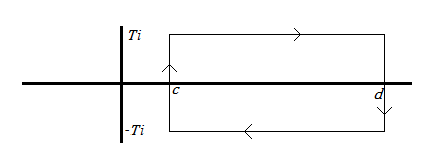
\includegraphics{analytic-chapters/dir-c1.png}
\end{figure}

Hence,
\begin{align*}
\ab{\int_{c-iT}^{c+iT}y^s\frac{ds}{s}}
&=\ab{\int_{c+iT}^{d+iT} y^s\frac{ds}{s}+\int_{d-iT}^{c-iT} y^s\frac{ds}{s}+\int_{d+iT}^{d-iT} y^s\frac{ds}{s}}\\
&\le 2\int_c^d y^{\si}\frac{d\si}{T}+\ab{\int_{d+iT}^{d-iT} y^s\frac{ds}{s}}.
\end{align*}
Note that the last integral goes to 0 as $d\to \iy$, because $|y^s|=|y^d|\to 0$. Hence, taking $d\to \iy$ gives
\[
\ab{\int_{c-iT}^{c+iT}y^s\frac{ds}{s}}
\le 2\int_c^{\iy} \frac{y^{\si}}{T}\,d\si=-\frac{2y^c}{T\ln y}=\frac{2y^c}{T|\ln y|}.
\]
This gives $\ab{\rc{2\pi i}\int_{c-iT}^{c+iT} y^s\frac{ds}{s}}\le \frac{y^c}{\pi T}{|\ln y|}$.

%Now we show the bound $\ab{\rc{2\pi i}\int_{c-iT}^{c+iT} y^s\frac{ds}{s}}\le \frac{y^c}{2}$, for any $y$.
By Cauchy's theorem applied to the smaller segment bounded by $\Re s=c$ and the circle with radius $R=\sqrt{c^2+T^2}$,  \fixme{(picture)} we have
\begin{align*}
%\int_{c-iT}^{c+iT} y^s\frac{ds}{s}+\int_C \frac{y^s}\frac{ds}{s}&=0\\
\ab{\int_{c-iT}^{c+iT} y^s\frac{ds}{s}}
&= \ab{\int_C y^s\frac{ds}{s}}\\
&\le \pi R\frac{y^{c}}{R}=\pi y^c,
\end{align*}
since $y<1$ and $\Re s>c$ on the arc. Hence $\ab{\rc{2\pi i}\int_{c-iT}^{c+iT} y^s\frac{ds}{s}}\le \frac{y^c}2$.\\

For $y>1$, take $d<0$. Note $\frac{y^s}{s}$ is analytic in the region below except for a simple pole at 0 with residue 1 (since $y^s=1$ when $s=0$). Hence by Cauchy's Theorem,
\[
\int_{c-iT}^{c+iT} y^s\frac{ds}{s}+\int_{c+iT}^{d+iT} y^s\frac{ds}{s}+\int_{d+iT}^{d-iT} y^s\frac{ds}{s}+\int_{d-iT}^{c-iT} y^s\frac{ds}{s}=2\pi i.
\]

\fixme{[INSERT PICCY]}

Then 
\begin{align*}
\ab{\int_{c-iT}^{c+iT}y^s\frac{ds}{s}-1}
&=\ab{\int_{c+iT}^{d+iT} y^s\frac{ds}{s}+\int_{d-iT}^{c-iT} y^s\frac{ds}{s}+\int_{d+iT}^{d-iT} y^s\frac{ds}{s}}\\
&\le 2\int_d^c y^{\si}\frac{d\si}{T}+\ab{\int_{d+iT}^{d-iT} y^s\frac{ds}{s}}.
\end{align*}
The last term goes to 0 as $d\to -\iy$, so the same argument applies as in the first part to show $\ab{\rc{2\pi i} \int_{c-iT}^{c+iT}y^s\frac{ds}{s}-1}\le \frac{y^c}{\pi T\ln y}$.

By Cauchy's theorem applied to the larger segment bounded by $\Re s=c$ and the circle with radius $R=\sqrt{c^2+T^2}$, \fixme{(picture)} we have
\begin{align*}
\int_{c-iT}^{c+iT} y^s\frac{ds}{s}+\int_C y^s\frac{ds}{s}&=2\pi i\\
\ab{\int_{c-iT}^{c+iT} y^s\frac{ds}{s}-1}
&\le \ab{\int_C y^s\frac{ds}{s}}\\
&\le 2\pi R\frac{y^{c}}{R}=2\pi y^c,
\end{align*}
since $y>1$ and $\Re s<c$ on the arc. Hence $\ab{\rc{2\pi i}\int_{c-iT}^{c+iT} y^s\frac{ds}{s}}\le y^c$.\\

Proof for $y=1$ omitted.
\end{proof}
\begin{cor}\llabel{sum-coeff-Dir}
The partial sum of the coefficients of a Dirichlet series is given by 
\[
\sum_{n<x} a_n+\frac{a_x}{2}(x\in \N_0)=\rc{2\pi i} \lim_{T\to \iy}\int_{c-iT}^{c+iT} x^s f(s)\frac{ds}{s}.
\]
The error from truncating the integral is
\[
\ab{\pa{\sum_{n<x} a_n+\frac{a_x}{2}(x\in \N_0)}-\pa{\rc{2\pi i} \int_{c-iT}^{c+iT} x^s f(s)\frac{ds}{s}}}\le \sum_{n=1}^{\iy} \pf xn^c a_n\min\pa{1,\rc{T\ab{\ln\pf xn}}}.
\]
\end{cor}


%%%%%%%%%%%%
\chapter{Zeta functions and the prime number theorem}\llabel{zeta-l-pnt}
\index{prime number theorem}
\section{Prime number theorem: Outline}
\begin{df}
Define the prime-counting function
\[
\pi(x)=|\set{p\le x}{p\text{ prime}}|.
\]
\end{df}
Our goal in this chapter is to prove the following famous theorem (in all its error-bounded glory).
\begin{thm}[Prime number theorem]\llabel{pnt}
There is an effective constant $C>0$ such that
\[
\pi(x)=\text{li}(x)+O(xe^{-C\sqrt{\ln x}})
\]
for all $x\ge 1$.
\end{thm}
Here $\Li(x)$ denotes the \textbf{logarithmic integral}
\[
\Li(x)=\int_2^x \frac{dt}{\ln t}.
\]
Note that $\Li(x)= \frac{x}{\ln x}+O\pf{x}{(\ln x)^2}$ as $x\to \iy$, since integration by parts gives
\begin{align}
\nonumber\li(x)&=\int_2^x \frac{dy}{\ln y} +O(1)=\frac{x}{\ln x}+\int_2^x \frac{dy}{(\ln y)^2}+O(1)\\
&=\frac{x}{\ln x}+O\pf{x}{(\ln x)^2}.\llabel{li-ibp}
\end{align}

\subsection{The big picture}

We recommend Andrew Granville's article IV.2 Analytic Number Theory in~\cite{PCTM} for an overview.

How might we guess at the asymptotics for $\pi(x)$? (In particular, why is it closer to $\Li(x)$ than $\fc{x}{\ln x}$?) By studying tables of primes up to 3 million, Gauss hypothesized that the density of primes at around $x$ is around $\rc{\ln x}$, and hence that the number of primes up to $x$ would be the integral $\Li(x)=\int_2^x \frac{dt}{\ln t}$. Making a table of $\pi(x)$ and the difference $\Li(x)-\pi(x)$, we find that the difference is slightly more than on the order of $\sqrt x$, so this seems to be a good estimate.

It is a common theme in analytic number theory to make conjectures about the distribution of primes (or other subsets of interest) by assuming they are randomly distributed according to some probability model. Often a simple model works for simple asymptotics up to $x$, and the model needs to be refined or corrected when dealing with more complicated quantities such as number of primes in a small interval, or spacing between primes.

\begin{mdl}[Gauss-Cram\'er model]
For $n\ge 3$, let $X_n$ be the random variable such that
\begin{align*}
X_n&=1 \text{ with probability }\rc{\ln n}\\
X_n&=0 \text{ with probability }1-\rc{\ln n}.
\end{align*}
Then the sequence $X_n$ behaves similarly to the sequence 
\begin{align*}
a_n&=1 \text{ if $n$ is prime}\\
a_n&=0 \text{ otherwise.}
\end{align*}
\end{mdl}
The Gauss-Cram\'er model exactly predicts $\pi(x)\sim \Li(x)$. The model gives more than just the asymptotics of $\pi(x)$, though, it can also be used to think about primes in short intervals $\pi(x+y)-\pi(x)$. \\

\prbbox{What are the shortcomings of the Gauss-Cram\'er model?}
\vskip0.15in

\subsection{Main steps}
The main steps in the proof are as follows.
\begin{enumerate}
\item When we have a Dirichlet series
\[
F(s)=\sum_{n=0}^{\iy} a_n n^{-s},
\]
we can get estimates for $\sum_{n=0}^N a_n$ by ``plucking out" those coefficients: The equation %using the Mellin transform:
\[
\rc{2\pi i}\lim_{T\to\iy}\int_{c-iT}^{c+iT} y^s\frac{ds}{s}=\begin{cases}
1,&\text{if }y>1\\
\rc 2,&\text{if }y=1\\
0,&\text{if }y<1.
\end{cases}
\]
gives
\[
\rc{2\pi i} \lim_{T\to \iy}\int_{c-iT}^{c+iT} x^s f(s)\frac{ds}{s}=\sum_{n<x} a_n+\frac{a_x}{2}(x\in \N_0).
\]
We use the more precise statement giving error bounds (Corollary~\ref{dirichlet}.\ref{sum-coeff-Dir}).

We want a Dirichlet series where the sum of the first $N$ terms is related to $\pi(N)$.
Let
\[
\ze(s)=\prod_{p\text{ prime}} \rc{1-p^{-s}}=\sum_{n=1}^{\iy}\rc{n^s}.
\]
We consider the function
\[
-\frac{\zeta'(s)}{\zeta(s)}=\sum_{p\text{ prime}} \frac{(\ln p)p^{-s}}{1-p^{-s}}
=\sum_{n=1}^{\iy} \La(n)n^{-s}.
\]
We use this function because $\psi(x):=\sum_{n<x} \La(n)$ gives information on $\pi(x)$, and 
$-\frac{\zeta'}{\zeta}$ continues into a meromorphic function on $\C$ (since $\ze$ does). We now have the estimate
\[
\psi(x)=\rc{2\pi i}\int_{c-iT}^{c+iT} -\frac{\zeta'(s)}{\zeta(s)} x^s\frac{ds}{s}+(\text{error}).
\]
\item We know $\zeta$ has analytic continuation (Theorem~\ref{zeta-continues}). Hence we can move the path of integration to $c<0$. From Cauchy's integral formula, we get extra terms from the horizontal integrals (integrals involving $-\frac{\zeta'}{\zeta}$) and terms $\frac{x^{\rho}}{\rho}$ from Cauchy's integral theorem from the zeros of $\zeta(s)$. {\it This is why we care about its zeros!} Zeros with large real part contribute large error terms.
We will need the following.
\begin{enumerate}
\item
We apply the product development (Theorem~\ref{complex-analysis}.\ref{product-development}) on $\xi(s)=\pi^{-\frac s2}\zeta(s)\Ga\pf s2$ to obtain
\[
\frac{\zeta'(s)}{\zeta(s)}=\sum_{\rh\text{ zero of }\zeta}\pa{\rc{s-\rh}+\rc{\rh}}+\cdots
\]
(Theorem~\ref{xi-product-development}).
%\[
%\frac{\ze'(s)}{\ze(s)}=\sum_{|T-\Im \rh|<1}\rc{s-\rh}+O(\ln T).
%\]
%(See Theorem~\ref{zeta-l-pnt}.\ref{zeta-product-development}).
\item
Using the above equation for $\frac{\zeta'}{\zeta}$, we calculate the asymptotics of $N(T)$, the number of zeros in $\set{\si+it}{(\si,t)\in[0,1]\times[-T,T]}$ (Theorem~\ref{zeta-zeros}).
\item
From (a) to (b) we get a zero-free region for $\ze$ (which includes $\Re s\ge 1$) (Theorems~\ref{weak-zeta-zeros} and \ref{zeta-zero-free}).
\end{enumerate}
From the zero-free region we get a bound for $\sum\frac{x^{\rh}}{\rh}$, as well as the horizontal integrals. 
If the Riemann hypothesis is true, then we can enlarge our zero-free region to $\Re s> \rc2$, which is even better. 
\item Finally we use the estimate for $\psi(x)$ to get an estimate for $\pi(x)$ (Lemma~\ref{partial-sum-pi}).
\end{enumerate}
\index{zeta function}
%\index{zeta function|Riemann}
%\index{zeta function|Hurwitz}
\section{Riemann zeta function}
\begin{df}
The \textbf{Riemann zeta function} is defined by %, the $L$-function with character $\chi$, and the \textbf{Hurwitz zeta function}, are respectively given by
%\begin{align*}
\[
\zeta(s)=\sum_{n=1}^{\iy} \rc{n^s}
%L(s,\chi)&=\sum_{n=1}^{\iy} \frac{\chi(n)}{n^s}\\
%\zeta(s,a)&=\sum_{n=0}^{\iy} \rc{(n+a)^s},&0<a\le 1.
%\end{align*}
\]
when $\Re s>1$. This will be generalized to $L$-functions $L(s,\chi)$ in Definition~\ref{l-func-dirichlet}.\ref{l-func-def}.
\end{df}
%Note that the $L$-function and $\zeta(s,a)$ are generalizations of $\zeta$ in different directions.
%Note
%\[
%L(s,\chi)=k^{-s}\sum_{r=1}^k \chi(r)\zeta\pa{s,\frac rk}.
%\]
By Theorem~\ref{euler-product} and by unique factorization in $\Z$, we can write
\[
\ze(s)=\prod_{p\text{ prime}}\rc{1-p^{-s}}.
\]
By taking the logarithmic derivative, we have %(VALID BY...), we have
\[
-\frac{\zeta'(s)}{\zeta(s)}=\sum_p \frac{d}{ds}\ln(1-p^{-s})
=\sum_p (\ln p)\frac{p^{-s}}{1-p^{-s}}=\sum_p \ln p\sum_{k=1}^{\iy} p^{-ks}.
\]
Interchanging order of summation gives
\begin{equation}\llabel{log-diff-zeta}
-\frac{\zeta'(s)}{\zeta(s)}=\sum_{n=1}^{\iy} \La(n)n^{-s}, \quad \Re s>1,
\end{equation}
where the von Mangoldt function $\La(n)$ is defined as
\[
\La(n)=\begin{cases}
\ln p,&n=p^r,\,p\text{ prime, }r\in \N.\\
0,&\text{else}
\end{cases}
\]

The most important property of $\ze$ is its analytic continuation and functional equation.
\begin{thm}\llabel{zeta-continues}
$\zeta(s)$ can be analytically continued to a meromorphic function with a simple pole at $s=0,1$. %with residue 1. 
It satisfies the functional equation
\[
\zeta(s)=2(2\pi)^{s-1}\Ga(1-s)\sin\pf{\pi s}2 \zeta(1-s).
\]
Letting $\xi(s)=\pi^{-\frac s2}\zeta(s)\Ga\pf s2$, we have\footnote{The factor $\Ga\pf s2$ can be thought of as coming from the infinite place---see Chapter~\ref{l-nf}.}
\[
\xi(s)=\xi(1-s).
\]
Moreover, $\ze(s)$ has zeros $-2\N$ (the trivial zeros); all other zeros are in the critical strip $0\le \Re s\le 1$.
\end{thm}
To prove this, we first need the transformation law for the theta function; we will show the functional equation for $\ze$ by writing it in terms of $\te$. As we will prove a more generalized transformation law, we will postpone the proof for $\te$.
\begin{df}
Define the \textbf{theta function} by
\[
\te(u)=\sum_{n\in \Z}e^{-\pi n^2u},\quad \Re u>0.
\]
\end{df}
\begin{pr}[Transformation law for $\te$]\llabel{theta-law}
For all $u$ with $\Re u>0$,
\[
\te\prc u = u^{\rc2} \te(u).
\]
\end{pr}
This is a special case of Proposition~\ref{l-func-dirichlet}.\ref{theta-transforms}.
\begin{proof}[Proof of Theorem~\ref{zeta-continues}]
We first analytically continue $\zeta$ to $\Re s>0$, show the functional equation is true for $0<\Re s<1$, and use it to establish analytic continuation to $\C$.

Note
\begin{equation}\llabel{continue-zeta-to-0}
\zeta(s)=\rc{s-1}+\sum_{n=1}^{\iy}\ba{
n^{-s}-\int_n^{n+1} x^{-s} \,dx
}
=\rc{s-1}+\sum_{n=1}^{\iy} \int_n^{n+1} (n^{-s}-x^{-s})\,dx
\end{equation}
Since for $n\le x\le n+1$ we have
\begin{align}
\nonumber|n^{-s}-x^{-s}|&=\ab{\int_{n}^x sx^{-s-1}\,dx}
\le|s|n^{-s-1}\\
\llabel{bound-zeta-summands}
\ab{\int_n^{n+1} n^{-s}-x^{-s}\,dx}&\le |s|n^{-s-1},
\end{align}
the sum~(\ref{continue-zeta-to-0}) converges uniformly locally for $\Re s>0$ and extends $\zeta$ to an analytic function for $\Re s>0$.

We claim that
\begin{equation}\llabel{zeta-theta}
2\xi(s)=\int_0^{\iy} (\theta(u)-1)u^{\frac s2} \frac{du}{u},\quad \Re s>1
\end{equation}
%i.e. $\zeta(-2s)$ is the Mellin transform of $\frac{\theta(u)-1}2$.
Indeed, we have
\begin{align*}
\int_0^{\iy} (\theta(u)-1)u^{\frac s2} \,\frac{du}u
&=\int_0^{\iy} 2\sum_{n=1}^{\iy} e^{-\pi n^2u}u^{\frac s2}\frac{du}u\\
&=2\sum_{n=1}^{\iy} \int_0^{\iy} e^{-\pi n^2u}u^{\frac{s}2}\,\frac{du}u\\%absolute convergence?
&=2\sum_{n=1}^{\iy} \int_0^{\iy} e^{-u} \pf{u}{\pi n^2}^{\frac s2}\,\frac{du}u&u\mapsfrom \frac{u}{\pi n^2}\\
&=2\pi^{-\frac s2}\pa{\sum_{n=1}^{\iy} \rc{n^s}}\pa{\int_0^{\iy} e^{-u} u^{\frac s2}\,\frac{du}u}\\
&=2\pi^{-\frac s2} \zeta(s)\Ga\pf{s}2=2\xi(s).
\end{align*}
The theta transformation law~\ref{theta-law} give that for $\Re s>1$,
\begin{align*}
2\xi(s)&=\int_0^1 (\theta(u)-1)u^{\frac s2}\frac{du}u
+\int_1^{\iy} (\theta(u)-1)u^{\frac s2} \frac{du}{u}\\
&=%-\frac{2}{s}+
\int_1^{\iy} \pa{\theta\prc u-1}u^{\frac s2} \frac{du}u +\int_1^{\iy} (\theta(u)-1)u^{\frac s2}\frac{du}u&u\mapsfrom \rc u\\
&=\int_1^{\iy}\pa{u^{-\rc2}\te\prc u-1} u^{\frac{1-s}2}\frac{du}u+\int_1^{\iy}(u^{\fc{1-s}2}-u^{-\fc{s}2})\fc{du}u
+\int_1^{\iy} (\theta(u)-1)u^{\frac s2}\frac{du}u\\
&=-\frac{2}{s}-\frac{2}{1-s}+\int_1^{\iy} (\theta(u)-1)u^{\frac{1-s}2}\frac{du}u+\int_1^{\iy}(\te(u)-1) u^{\frac s2}\frac{du}u.
\end{align*}
The last expression converges for all $\Re s>0$, so in fact equals $2\ze(s)$ for all $\Re s>0$ by uniqueness of analytic continuation. Since the last expression is symmetric under $1-s\mapsto s$, the functional equation for $\xi$ follows.

%To get the functional equation for $\ze$, note
The functional equation for $\xi$ gives
\begin{align*}
\ze(s)&=\pi^{\fc s2} \Ga\pf s2^{-1}\pi^{-\fc{1-s}2} \Ga\pf{1-s}2\ze(1-s)\\
&=\pi^{s-\rc2} \frac{\Ga\pf{1-s}2}{\Ga\pf{s}2}\ze(1-s)\\
&=\pi^{s-\rc2}\Ga\pf{1-s}2 \Ga\pa{1-\fc s2} \frac{\sin\pf{\pi s}2}{\pi}\ze(1-s)&\text{by Proposition~\ref{complex-analysis}.\ref{gamma-facts}(5)}\\
&=2(2\pi)^{s-1}\sin\pf{\pi s}2\Ga(1-s)\ze(1-s)&\text{by Proposition~\ref{complex-analysis}.\ref{gamma-facts}(6)}
\end{align*}

Finally, the statement about zeros follows from the fact that $\ze$ has no zeros with $\Re s>1$ (as $\fc{\ze'}{\ze}$ is holomorphic there) and the functional equation, noting $\sin\pf{\pi s}{2}=0$ exactly when $s$ is an even integer, with the zero at $s=0$ cancelled by the pole at 1 of $\ze$.
\end{proof}
\begin{thm}[Product development of $\xi$]\llabel{xi-product-development}
The function $(s^2-s)\xi(s)$ is entire of order 1, and $\xi(s)$ has the product expansion
\[
\xi(s)=\frac{e^{A+Bs}}{s^2-s}\prod_{\rho\text{ zero of }\ze} \pa{1-\frac s{\rh}}e^{\frac s{\rh}}.
\]
Then $\frac{\zeta'}{\zeta}(s)$ has the partial-fraction expansion
\[
\frac{\zeta'}{\zeta}(s)=B-\rc{s-1}+\rc{2}\ln(\pi) -\rc2\frac{\Ga'}{\Ga}\pa{\frac s2+1}+\sum_{\rh\text{ nontrivial zero of }\zeta}\pa{\rc{s-\rh}+\rc{\rh}}.
\]
\end{thm}
From now on, unless otherwise specified, when we say zero of $\ze$ we mean {\it nontrivial} zero.
\begin{proof}
Note $(s^2-s)\xi(s)$ is entire because $\xi$ only has 2 simple poles at $0,1$. To show it has order 1 we need two inequalities.\\

\noindent \underline{Step 1:} There is no constant $C$ so that $(s^2-s)\xi(s)\precsim e^{C|s|}$: Indeed, for real $s$ and any constant $C$, by Stirling's approximation~\ref{complex-analysis}.\ref{stirling} we have
\begin{align*}
(s^2-s)\xi(s)&=(s^2-s)\pi^{-\frac s2}\Ga\pf s2\ze(s)\\
&\succsim s^{-\rc 2}\pf{s}{2e\pi}^{\frac s2}
\succsim e^{Cs}.
\end{align*}
\noindent\underline{Step 2:} There is a constant $C$ so that $(s^2-s)\xi(s)\precsim e^{C|s|\ln|s|}$: $e^{|s|\ln|s|}\ge1$ for all $s$ so it suffices to prove this for sufficiently large $s$. By the integral and sum formulas for $\Ga$ and $\xi$, and the fact that $|x^s|=|x^{\Re s}|$, we have
\[
|\xi(\si+ti)|\le \pi^{-\frac{\si}{2}}\Ga\pf{\si}{2}\ze(\si),\quad \si>1.
\]
By symmetry of $\xi$ is suffices to consider $\si\ge \rc2$. (``Nudging" $|s|$ in $e^{C|s|\ln|s|}$ by a constant changes it by at most a constant factor.)
Consider 2 cases.
\begin{enumerate}
\item
$\si>2$: Then $\pi^{-\frac{\si}{2}}<1$ and $\ze(\si)<\ze(2)$ so by Stirling's approximation~\ref{complex-analysis}.\ref{stirling},
\[
|\xi(\si+ti)|\precsim
\Ga\pf{\si}2
%\precsim %\pf{\si}{2}^{\frac{\si}2-\rc 2}e^{-\frac{\si}{2}}
=e^{|(\ln\Ga)(\si)|}=e^{\pa{\frac{\si}2-1}\ln\frac{\si}2-\frac{\si}2+O(1)}
\]
from which the result follows.
\item
$\frac12\le \si\le 2$: From~(\ref{bound-zeta-summands}), we have for $s$ bounded away from 1,
\[
\zeta(s)\le O(1)+|s| \sum_{n=1}^{\iy} n^{-\frac 32}=O(|s|).
\]
This time $\Ga\pf{\si}{2}=O(1)$ so
\[
|(s^2-s)\xi(s)|\le \ab{
s^2\pi^{-\frac{\si}2}\zeta(s)\Ga\pf{\si}2}
=O(|s|^3)\precsim e^{C|s|\ln|s|}.
\]
\end{enumerate}
This shows $(s^2-s)\xi(s)$ has order 1.\\

\noindent\underline{Step 3:} By the product development~\ref{complex-analysis}.\ref{product-development}, noting the the zeros of $(s^2-s)\xi$ are the nontrivial zeros of $\ze$ (since $\Ga$ has no zeros and trivial zeros of $\ze$ come from the poles of $\Ga$ in the definition of $\xi$), we get
\[
(s^2-s)\xi(s)=e^{A+Bs}\prod_{\rh\text{ zero of }\zeta}\pa{1-\frac{s}{\rh}}e^{\frac s{\rh}}.
\]
Dividing by $s^2-s$ and log-differentiating gives
\[
\frac{\xi'}{\xi}(s)=B-\rc{s}-\rc{s-1}+\sum_{\rh} \pa{\rc{s-\rh}+\rc{\rh}}.
\]
Since $\ze(s)=\pi^{\frac s2}\Ga\pf{s}2^{-1}\xi(s)$, we get
\begin{align*}
\frac{\ze'}{\ze}(s)&=\rc{2}\ln\pi +\rc2\frac{\Ga'}{\Ga}\pa{\fc s2}+B-\rc{s}-\rc{s-1}+\sum_{\rh} \pa{\rc{s-\rh}+\rc{\rh}}\\
&=\rc{2}\ln\pi +\rc2\frac{\Ga'}{\Ga}\pa{\fc s2+1}+B-\rc{s-1}+\sum_{\rh} \pa{\rc{s-\rh}+\rc{\rh}},&\Ga(z)=\fc{\Ga(z+1)}{z}.\qedhere
\end{align*}
\end{proof}
\section{Zeros of zeta}
Note that from the function equation, $\ze(s)$ has simple zeros at $-2\N$. We call these trivial zeros. More importantly for us are the zeros with real part in $[0,1]$.

Denote by $N(T)$ be the number of zeros of $\zeta$ in $\set{\si+it}{(\si,t)\in [0,1]\times [-T,T]}$, counting multiplicity. We first give asymptotics on the vertical distribution of zeros of $\zeta$ (von Mangoldt's formula, Theorem~\ref{zeta-zeros}), then give a zero-free region for $\zeta$ (Theorem~\ref{zeta-zero-free}).
\begin{lem}\llabel{weak-zeta-zeros}
Define $\cal L(t)=\ln (|t|+2)$. 
For $s=\si+it$ with $\si\in [-1,2]$, we have\footnote{Note $\rc{s-1}=O(1)$ when $s$ is bounded away from 1.}
\begin{align}
\llabel{weak-zeta-zeros-eq1}
\frac{\zeta'(s)}{\zeta(s)}
&={\color{gray}-\rc{s-1}}
+\sum_{\rh}\pa{\rc{s-\rh}+\rc{\rh}}+O(\cal L)\\
\nonumber
&={\color{gray}-\rc{s-1}}
+\sum_{|\Im(s-\rh)|<1} \rc{s-\rh} +O(\cal L).
\end{align}
Moreover, there are $O(\cal L)$ zeros $\rh$ with $|\Im(s-\rh)|<1$, i.e. the number of zeros with imaginary part in $[t,t+1]$ is $O(\ln t)$, as $t\to \iy$.
\end{lem}
Note this gives $N(T)=O(T\ln T)$. The next theorem will give an improvement of this estimate.
\begin{proof}
Our strategy is this: at a point where we know $\frac{\ze'}{\ze}$ is bounded ($s=2+it$), we use Theorem~\ref{xi-product-development} to get information on how many zeros of $\zeta$ can be close to $s$. Then we use compare $\frac{\ze'}{\ze}(\si+it)$ with $\frac{\ze'}{\ze}(2+it)$ to get the general estimate.\\

\noindent\underline{Step 1:}
Theorem~\ref{xi-product-development} gives us
\begin{equation}\llabel{zeta2-zero-sum}
\frac{\zeta'(s)}{\zeta(s)}=-\rc{s-1}+
\underbrace{B+\rc2\ln\pi}_{O(1)}
-
\rc2\underbrace{\frac{\Ga'}{\Ga}\pa{%\frac{\si}2+1+i\frac t2}
\frac s2+1}}_{(A)}+
\underbrace{\sum_{\rh} \pa{\rc{%\si+it
s-\rh}+\rc{\rh}}}_{(B)}.
\end{equation}
From Stirling's approximation~\ref{complex-analysis}.\ref{stirling}, (A) equals
\begin{equation}\llabel{gamma2-estimate}
%\underbrace{
\ln\ab{\frac{\si}{2}+1+i\frac t2}%}_{O(1+\ln |t|)}
+O(1)=
%\underbrace{\frac{1}{2\ab{\frac{\si}{2}+1+i\frac t2}}}_{O(1)}
%+O\pa{\ab{\frac{\si}{2}+1+i\frac t2}^{-2}}=
%O(\ln |t|).
O(\cal L)
\end{equation}
These two equations show~(\ref{weak-zeta-zeros-eq1}).

Now suppose $s=2+it$. %Theorem~\ref{xi-product-development} says
Note that
\[
\ab{\frac{\ze'(2+it)}{\ze(2+it)}}
=\ab{\sum_{n=1}^{\iy} \La(n)n^{-2-it}}
\le \ab{\sum_{n=1}^{\iy} (\ln n)n^{-2}}<\iy,
\]
so the LHS of~(\ref{zeta2-zero-sum}) is $O(1)$.
%%%%%%
%Now we estimate (B) by truncating the sum.
Hence~(\ref{zeta2-zero-sum}) becomes
\begin{equation}\llabel{zeta2-zero-sum2}
O(\cal L)=\sum_{\rh} \pa{\rc{%\si+it
s-\rh}+\rc{\rh}}.
\end{equation}
%Note
%\[
%\Re\pa{\rc{2+it-\rh}+\rc{\rh}}=\Re\pa{
%\frac{(2+\Re \rh)-(t-\Im \rh)i}{(2-\Re \rh)^2+(t-\Im\rh)^2}
%}
%\ge\rc{4+(t-\Im \rh)^2}
%\]
%since $0\le \Re \rh\le 1$.
We estimate the terms with $|\Im(s-\rh)|<1$ by a constant to show that there aren't too many of them.
From~(\ref{zeta2-zero-sum2}) and~(\ref{gamma2-estimate}),
\begin{align}
%O(\ln |t|) &\ge \Re\sum_{|\Im(s-\rh)|<1}\pa{\rc{2+it-\rh}+\rc{\rh}}\\
%%&\ge \Re\sum_{
%%%{\footnotesize\begin{array}{c}
%%%\rh\text{ zero}\\
%%|\Im(s-\rh)|<1%\end{array}}}
%%}\frac{(2+\Re \rh)-(t-\Im \rh)i}{(2-\Re \rh)^2+(t-\Im\rh)^2}\\
%&=\sum_{|\Im(s-\rh)|<1}\rc{4+(t-\Im \rh)^2}\\
%&\ge \rc 5 |\set{\rh}{|\Im(s-\rh)|<1}|.
%
\nonumber
O(\cal L) &= \Re\sum_{\rh}\pa{\rc{2+it-\rh}+\rc{\rh}}\\
\nonumber
&\ge
\Re\sum_{\rh}\pa{
\frac{(2-\Re \rh)-(t-\Im \rh)i}{(2-\Re \rh)^2+(t-\Im\rh)^2}
}&\text{since }\Re \prc{\rh}>0\\
\nonumber
&\ge\sum_{\rh} \rc{4+(t-\Im \rh)^2}&\text{since $0\le \Re \rh\le 1$}\\
\llabel{zero-olnt}
&\ge \rc 5 |\set{\rh}{|\Im(s-\rh)|<1}|+\rc5 \sum_{|\Im(s-\rh)|\ge 1}\rc{(t-\Im \rh)^2}.
\end{align}
This proves the second part of the lemma.\\
%%We similarly consider the sum for $|\Im(s-\rh)|>1$:
%%\begin{align}
%%\llabel{olntge}
%%O(\ln|t|)
%%&\ge\sum_{|\Im(s-\rh)|\ge 1}\pa{\rc{2+it-\rh}+\rc{\rh}}\\
%%\nonumber&=\sum_{|\Im(s-\rh)|<1}\rc{4+(t-\Im \rh)^2}\\
%%\nonumber&\ge \rc5 \sum_{|\Im(s-\rh)|<1}\rc{(t-\Im \rh)^2}
%%\end{align}
%Now from~(\ref{zeta2-zero-sum}),
%\begin{align*}
%\ab{\frac{\zeta'(2+it)}{\zeta(2+it)}}
%%O(\ln|t|)
%&=\sum_{|\Im(s-\rh)|<1}\rc{s-\rh}+
%\underbrace{\sum_{|\Im(s-\rh)|<1}\rc{\rh}}_{O(\ln|t|)}
%+
%\underbrace{\sum_{|\Im(s-\rh)|\ge 1}\pa{\rc{2+it-\rh}+\rc{\rh}}}_{O(\ln|t|)}
%%&=O(\ln|t|)+\sum_{|\Im(s-\rh)|<1}\rc{s-\rh}+O(\ln|t|)+O(\ln|t|),
%\end{align*}
%as needed. (The first $O(\ln|t|)$ is because there are $O(\ln|t|)$ terms in the sum and each is at most 1 in absolute value.)\\

\noindent\underline{Step 2:} Now we consider general $s=\si+it$, by comparing it to $2+it$. We have by~(\ref{zeta2-zero-sum}) and~(\ref{gamma2-estimate}) that
\begin{align*}
&\quad \frac{\zeta'}{\zeta}(s)-\underbrace{\frac{\ze'}{\ze}(2+it)}_{O(1)}\\
&=-\rc{s-1}+O(1)+\underbrace{\rc2\pa{\ln\ab{\frac{\si}2+1+\frac t2i}-
\ln\ab{2+\frac t2i}}}_{O(1)}+\sum_{\rh} \pa{\rc{s-\rh}-\rc{2+it-\rh}}\\
&=-\rc{s-1}+O(1)+
\sum_{|\Im(s-\rh)|<1}\rc{s-\rh}-\underbrace{\sum_{|\Im(s-\rh)|<1}\rc{2+it-\rh}}_{O(\cal L)}+
\underbrace{\sum_{|\Im(s-\rh)|\ge1}\frac{(2-\si)}{(s-\rh)(2+it-\rh)}}_{O(\cal L)}.
\end{align*}
The first $O(\cal L)$ is because there are at most $O(\cal L)$ terms and each term is at most 1 in absolute value; the second is from
\[
\sum_{|\Im(s-\rh)|\ge1}\frac{2-\si}{(s-\rh)(2+it-\rh)}=O\pa{\sum_{|\Im(s-\rh)|\ge1}\frac{1}{\Im(s-\rh)^2}}=O(\cal L);
\]
the first equality is from $2-\si=O(1)$ and $\Im(s-\rh)=\Im(2+it-\rh)$; the second is by~(\ref{zero-olnt}).
\end{proof}
\index{von Mangoldt's Theorem}
\begin{thm}[von Mangoldt]\llabel{zeta-zeros}($*$) 
As $T\to \iy$,
\[
N(T)=\frac{T}{\pi}\ln\pf{T}{2\pi}-\frac{T}{\pi}+O(\ln T).
\]
\end{thm}
\begin{proof}
As $\zeta$ has only a countable number of zeros, we may assume $T$ is not the imaginary part of any zero.

Let
\[
\cal R=\set{\si+it}{(s,t)\in [-1,2]\times [-T,T]}
\]
and let $C$ be the boundary of $\cal R$. \fixme{(PICTURE)}
%Since $\Ga(\ol s)=\ol{\Ga(s)}$, the zeros of $\Ga$ are symmetric across the real axis. 
From $\xi(s)=\pi^{-\frac s2}\zeta(s)\Ga\pf s2$, we see that $\xi$ has the same zeros as $\zeta$ in this region, and simple poles at $0$ and $1$. %Now $\Ga$ has $2N(T)$ zeros (note it has no zeros on the real axis)
%and $2$ poles in $\cal R$, namely $0$ and $1$. 
Hence by Cauchy's residue formula~\ref{complex-analysis}.\ref{residue},
\[
\rc{2\pi i}\oint_{C} \frac{\xi'(s)}{\xi(s)} ds=2N(T)-2.
\]
Noting that $\xi(\ol{s})=\ol{\xi(s)}$ and $\xi(s)=\xi(1-s)$, changes of variable show that the integral on each of the sections of $C$ between $2$, $\rc 2+iT$, $-1$, and $\rc 2-iT$ are the same.\footnote{We used $\xi$ because its symmetry allows us to do this.} Let $C'$ be the part from $1$ to $\rc 2+iT$. Thus 
%(using $\pa{\prod_{k=1}^n f_k}'=\sum_{k=1}^n \frac{f_k'}{f_k}$), 
the above equals
\begin{align*}
\frac2{\pi i}\int_{C'} \frac{\xi'(s)}{\xi(s)} ds
&=\frac2{\pi i}
\int_{C'} -\frac{\ln \pi}{2}+\frac{\zeta'(s)}{\zeta(s)}+\frac{\pa{\Ga\pf{s}{2}}'}{\Ga\pf s2}\,ds&\frac{\pa{\prod_{k=1}^n f_k}'}{\prod_{k=1}^n f_k}=\sum_{k=1}^n \frac{f_k'}{f_k}\\
&=\frac2{\pi}\Im
\int_{C'} -\frac{\ln \pi}{2}+\frac{\zeta'(s)}{\zeta(s)}+\frac{\pa{\Ga\pf{s}{2}}'}{\Ga\pf s2}\,ds
&\text{(expression is real)}.
\end{align*}
We break this up into 3 integrals and estimate each part separately.
\begin{enumerate}
\item $\Im\int_{C'}-\frac{\ln \pi}{2}\,ds=-\frac{T}{2}\ln \pi$.
\item Using the estimate for $\frac{\zeta'}{\zeta}$ in Lemma~\ref{weak-zeta-zeros},  we evaluate the second integral. Note that $\ln\zeta$ is defined for $\Re s> 1$ and is uniformly bounded for $\Re s=2$:
\begin{align*}
(\ln\zeta)(s)&=\sum_{p\text{ prime}} \ln(1-p^{-s}) \\
|(\ln\zeta)(2+it)|&\le\sum_{p\text{ prime}} 2p^{-2}.
\end{align*}
(Just bound $\ln$ linearly near 1, or expand in Taylor series.)  
Note $\ln(x-\rh)$ is well-defined on $C'$ for any $\rh$. Hence by Theorem~\ref{weak-zeta-zeros},
\begin{align*}
\Im\int_{C'}\frac{\zeta'}{\zeta}(s)\,ds
&=(\Im(\ln\zeta)(2+iT)-{\Im(\ln\zeta)(2)})+\int_{2+iT}^{\rc 2+iT} \frac{\zeta'}{\zeta}(s)\,ds\\
&=O(1)+\int_{2+iT}^{\rc 2+iT} \Im\pa{\sum_{|\Im(s-\rh)|<1}\rc{s-\rh}}+O(\ln T)\,ds\\
&=O(\ln T)+\sum_{|\Im(s-\rh)|<1}\Im(\ln(x-\rh))|^{\rc2+Ti}_{2+Ti}\\
&\le O(\ln T)+2\pi O(\ln T)
\end{align*}
since there are at most $\ln T$ terms in the sum.
\item We estimate the last integral using Stirling's formula~\ref{complex-analysis}.\ref{stirling}. (Note that $\ln\Ga$ is well-defined for $s\in C'$.)
\begin{align*}
\int_{C'}\frac{\pa{\Ga\pf s2}'}{\Ga\pf s2}
&=\ba{\Im(\ln\Ga)\pf s2}^{\rc 2+Ti}_2\\
&=\Im(\ln \Ga)\pa{\frac 14+\frac{T}{2}i}\\
&=\Im\ba{\pa{-\rc 4+\frac T2i}\ln\pa{\rc 4+\frac T2i}-\pa{\rc 4+\frac T2i}+O(1)}\\%&\text{by Theorem~\ref{complex-analysis}.\ref{stirling}}\\
&=\frac T2\ln\pf T2-\frac T2+O(1).&\qedhere
\end{align*}
\end{enumerate}
Now put everything together to get
\begin{align*}
N(T)-2&=\frac{2}{\pi}\pa{-\frac T2\ln \pi+O(\ln T)+\pa{\frac T2\ln\pf T2-\frac T2+O(1)}}\\
N(T)&=\frac{T}{\pi}\ln\pf{T}{2\pi}-\frac{T}{\pi}+O(\ln T).
\end{align*}
\end{proof}
\begin{thm}[Zero-free region for $\zeta$]\llabel{zeta-zero-free}
There are no zeros of $\zeta$ with $\Re s\ge 1$. Moreover, there is a constant $c>0$ such that for $|t|>2$, every zero $\si+it$ satisfies
\[
\si<1-\frac{c}{\ln|t|}.
\]
\end{thm}
\fixme{PICTURE!}
\begin{proof}
%(The proof of the first statement will give us motivation for the second.)
%We know that $\frac{\zeta'}{\zeta}$ has no pole for $\Re s>1$, and hence $\zeta$ has no zero for $\Re s>1$. Thus for the first part it suffices to prove that no zero has real part 1.
We already noted $\ze$ has no zero for $\Re s>1$ (Theorem~\ref{zeta-continues}), so for the first part it suffices to prove that no zero has real part 1.

If $\zeta$ had a zero $1+it$, then $\frac{\zeta'}{\zeta}$ would have a pole of positive residue at $1+it$. For $s=\si+it$, $\si>1$ we have $-\frac{\zeta'}{\zeta}(s)=\sum_{n=1}^{\iy} \frac{\La(n)}{n^s}$, so this means that as $\si\to 1^+$,
many of the important terms would have $n^{-it}$ ``close" to $-1$, to make it blow up in the negative direction. For those terms, we have $n^{-2it}$ ``close" to $1$. This would force $-\frac{\zeta'}{\zeta}(\si+2ti)$ to have a pole of positive residue at $1+2ti$, i.e $\zeta$ to have a pole at $1+2ti$, contradicting the fact that it is analytic there.

We now make this idea precise. What we want is an inequality between some function of an angle and its double, so that if one is small it forces the other to be large. So we consider
\[
0\le 2(1+\cos\theta)^2=3+4\cos \theta +\cos 2\theta.
\]
This gives
\[
0\le 3+4\Re(n^{-it})+\Re(n^{-2it}).
\]
Multiplying by $\La(n)n^{-\si}$ and summing, we get
\begin{equation}\llabel{zero-free-zeta-inequality}
0\le 3\pa{-\frac{\ze'}{\ze}(\si)} 
+4\Re\pa{-\frac{\ze'}{\ze}(\si+ti)}
+\Re\pa{-\frac{\ze'}{\ze}(\si+2ti)},\quad\si>1.
\end{equation}
Letting $r$ be the degree of the zero at $1+ti$, we have by Lemma~\ref{weak-zeta-zeros}
\[
0\le\pa{\frac{3}{\si-1}+O(1)}
-\pa{\frac{4r}{\si-1}+O(\cal L)}
+\Re\pa{-\frac{\ze'}{\ze}(\si+2ti)}\text{ as }\si\to 1^+.
\]
If $r\ge 1$, then this gives $-\frac{\ze'}{\ze}(\si+2ti)\to \iy$ as $\si\to 1^+$, contradiction. Hence $r=0$; $1+it$ is not a zero.

For the second statement, we have to use the partial fraction decomposition~\ref{xi-product-development}.
Suppose $\rh=(1-\de)+it$ is a zero. By Lemma~\ref{weak-zeta-zeros}, we have
\[
-\frac{\zeta'(s)}{\zeta(s)} = O(\ln|t|) -\sum_{\rh}\pa{\rc{s-\rh}+\rc{\rh}}\le O(\ln|t|)-\rc{s-\rh}.
\]
%(All terms in the last sum are positive.)
Then
\begin{align*}
-\Re\frac{\zeta'}{\ze}(\si+ti)&\le O(\ln|t|)-\frac{1}{\si+\de-1}\\
-\Re\frac{\zeta'}{\ze}(\si+2ti)&\le O(\ln|2t|)=O(\ln |t|).
\end{align*}
For $\si>1$, plugging this into~(\ref{zero-free-zeta-inequality}) gives
\begin{align*}
0&\le \frac{3}{\si-1}+O(\ln|t|)-\frac{4}{\si+\de-1}\\
\implies \frac{4}{\si+\de-1}&<\frac{3}{\si-1}+C_1\ln|t|
\end{align*}
for some $C_1$.
Now take $\si=1+4\de$ to get
\[
\frac{4}{5\de}<\frac{3}{4\de}+C_1\ln|t|,
\]
giving
\[
\de>\frac{1}{20C_1\ln|t|}
\]
as needed.
\end{proof}
\section{Prime number theorem: proof}
Now we gather everything together to prove the prime number theorem. We first show the following.
\index{von Mangoldt's formula}
\begin{thm}[von Mangoldt's formula]\llabel{von-Mangoldt-formula}
For an integer $x>2$ and $x\ge T$,
\begin{equation}\llabel{v-M-f}
\psi(x)= x-\sum_{|\Im(\rh)|<T}\frac{x^{\rh}}{\rh}
+O\pa{
\frac{x(\ln x)^2}{T}%+
%\frac{x(\ln T)^2}{T}+\ln x
}.
\end{equation}
\end{thm}
\begin{proof}
\noindent{\underline{Step 1:}} We estimate $\psi(x)$ using Theorem~\ref{dirichlet}.\ref{sum-coeff-Dir}. Suppose $x$ is an integer; the theorem gives
\begin{align*}
\ab{\psi(x)-\pa{
\int_{c-iT}^{c+iT} x^s\pa{-\fc{\ze'}{\ze}(s)\frac{ds}s
}}}&\le
\La(x)+
\sum_{n\ge 1,\,n\ne x} \pf xn^c\La(n)\rc{T\ab{\ln\pf xn}}\\
&\le 
\ln(x)+\sum_{n\ge 1,\,n\ne x}\pf xn^c\fc{\ln(n)}{T\ab{\ln\pf xn}}.
\end{align*}
%Assume $x$ is a large integer (i.e. bounded away from 1) and 
Take
\[
c=1+\rc{\ln x}.
\]
Note that this makes $x^c=ex=O(x)$. 
To estimate the sum we split it into several parts.
\begin{enumerate}
\item
$1\le n< \frac{x}{e}$: We have
\begin{align*}
\sum_{1\le n<\frac xe} \pf xn^c \frac{\ln n}{T\ab{\ln\pf xn}}
&\precsim \frac{x\ln x}{T}\sum_{1\le n<x}\rc{n}\\
&\sim \frac{x(\ln x)^2}{T}.
\end{align*}
\item
$\frac xe\le n< ex$: We have
\begin{align*}
\sum_{\frac xe\le n<ex,\,n\ne x}\pf xn^c \ln n\frac{1}{T\ab{\ln\pf xn}}
&\precsim \sum_{\frac xe\le n<ex,\,n\ne x} \cancel{e^{1+\rc{\ln x}}} \frac{\ln n}{T\ab{\ln\pf xn}}\\
&\precsim \rc{T}\sum_{\frac xe\le n<ex,\,n\ne x}\frac{\ln x}{\ab{1-\frac xn}}&\text{ using $\ln x\sim x-1$ when $x\approx 1$}\\
&\precsim \frac{x\ln x}{T}\sum_{\frac xe\le n<ex,n\ne x}\frac{1}{|n-x|}\\
&\precsim\frac{x\ln x}{T}\sum_{1\le n< (e-1)x}\frac{1}{n}\\
&\sim\frac{x(\ln x)^2}{T}.
\end{align*}
\item $n\ge ex$: We have
\begin{align*}
\sum_{n\ge ex} \pf xn^c \frac{\ln n}{T}&<\frac{x}{T}\int_{ex-1}^{\iy} \frac{\ln y}{y^c}\,dy&\frac{\ln y}{y^c}\text{ decreasing for }y>e\\
&=\frac xT\ba{\frac{-y^{-c+1}\ln y}{c-1}-\frac{y^{-c+1}}{(c-1)^2}}^{\iy}_{ex-1}\\
&\sim \frac{x(\ln x)^2}{T}.
\end{align*}
\end{enumerate}
Putting everything together gives
\begin{equation}\llabel{von-M-1}
\ab{\psi(x)-\pa{
\int_{c-iT}^{c+iT} x^s\pa{-\fc{\ze'}{\ze}(s)}\frac{ds}s
}}=O\pa{\frac{x(\ln x)^2}{T}+\ln x}.
\end{equation}

\noindent\underline{Step 2:} We move the line of integration to $\Re s=-1$. Assuming that $T$ is not the imaginary part of any root, by Cauchy's residue theorem~\ref{residue} \fixme{PICTURE}
\[
\int_{c-iT}^{c+iT} \frac{x^s}{s}\frac{\zeta'}{\ze}(s)\,ds
+\underbrace{\int_{c+iT}^{-1+iT} \frac{x^s}{s}\frac{\zeta'}{\ze}(s)\,ds}_{I_{h,1}}
+\underbrace{\int_{-1+iT}^{-1-iT} \frac{x^s}{s}\frac{\zeta'}{\ze}(s)\,ds}_{I_{v}}
+\underbrace{\int_{-1-iT}^{c-iT} \frac{x^s}{s}\frac{\zeta'}{\ze}(s)\,ds}_{I_{h,2}}
=\fc{\ze'}{\ze}(0)-x+\sum_{|\Im\rh|<T}\frac{x^{\rh}}{\rh}.
\]
Here $\fc{x^{\rh}}{\rh}$ are the resuides at the zeros, $-x$ comes from the pole of $\ze$ at 1, and $\fc{\ze'}{\ze}(0)$ comes from the pole of $\rc s$.
Then
\begin{equation}\llabel{von-M-2}
\int_{c-iT}^{c+iT} \frac{x^s}{s}\pa{-\fc{\zeta'}{\ze}(s)}\,ds-x=1+I_{h,1}+I_{h,2}+I_v-\sum_{\Im\rh<T}\frac{x^{\rh}}{\rh}.
\end{equation}
We estimate each summand.
\begin{enumerate}
\item For the horizontal integrals, we use the estimate~\ref{weak-zeta-zeros} to get
\begin{align*}
\ab{\frac{\ze'}{\ze}(s)}&=\ab{\sum_{|\Im(s-\rh)|<1} \rc{s-\rh}}+O(\ln T),\quad s=\si+Ti\\
&\le \sum_{|\Im(s-\rh)|<1}\rc{\Im(s-\rh)}+O(\ln T).
\end{align*}
We would like to bound $\Im(s-\rh)$ away from 0. To do this, note that there are $O(\ln T)$ roots in with $\Im \rh\in [T,T+1]$ by Lemma~\ref{weak-zeta-zeros}. Hence by tweaking $T$ slightly\footnote{Changing $T$ by a constant does not change the error term of~(\ref{v-M-f}); moreover the change in the LHS sum is $O\pa{\fc xT\ln T}=O\pf{x(\ln x)^2}T$.},
we can assume $|\Im(s-\rh)|>\frac{C}{\ln T}$ for all $\rh$. Also by Lemma~\ref{weak-zeta-zeros} there are at most $O(\ln T)$ terms in the sum, so the sum is $O((\ln T)^2)$.
Integrating gives
\begin{align*}
\ab{\int_{c\pm Ti}^{-1\pm Ti} \frac{x^s}{s}\frac{\ze'}{\ze}(s)ds}
%=\int_{c+Ti}^{1+Ti} O(\ln |T|)\,ds
&=O((\ln T)^2)O\prc T\int_{c}^{-1} |x^s|\,ds\\
&=O\pf{(\ln T)^2}{T}O(x)\\%\ab{\ba{\frac{x^s}{\ln x}}^{-1}_c}\\
&=O\pf{x(\ln x)^2}{T}.
\end{align*}
\item For the vertical integral, we use the same estimate, this time noting that $|s-\rh|>1$ for every root $\rh$, since every zero satisfies $\Re \rh>0$. This gives that $\frac{\ze'}{\ze}(s)=O(\ln T )$, and
\begin{align*}
\ab{\int_{-1+Ti}^{-1-Ti}
\frac{x^s}{s}\frac{\ze'}{\ze}(s)\,ds}
&=
O(\ln T )
\int_{-1-Ti}^{-1+Ti} \frac{x^{-1}}{|s|}\,ds
\\
&=
O\pf{\ln T  }{x}
\int_{-T}^{T} \rc{\sqrt{t^2+1}}\,dt\\
&=
O\pf{\ln T  }{x}
\int_{1}^{T+1} \rc{t}\,dt\\
&=
O\pf{(\ln T )^2}{x}=O\pf{x(\ln x)^2}{T}.
\end{align*}
\end{enumerate}
Equations~(\ref{von-M-1}) and~(\ref{von-M-2}) together with the above two estimates give the theorem.
\end{proof}
The final ingredient in the proof of the Prime Number Theorem is the estimate for $\sum_{|\Im(\rh)|<T}\frac{x^{\rh}}{\rh}$ using the zero-free regions for $\ze$ and the estimate for number of zeros of $\ze$.
\begin{proof}[Proof of Theorem~\ref{pnt}]
First, note there can only be a finite number of zeros of $\ze$ with $|\Im(\rh)|<2$, so $\sum_{|\Im(\rh)|<2}\frac{x^{\rh}}{\rh}=O(x^r)$ for some fixed $r<1$.\footnote{In fact, there are zero such zeros.} We estimate $\sum_{2\le |\Im(\rh)|<T}\frac{x^{\rh}}{\rh}$ in two steps.
\begin{enumerate}
\item By Theorem~\ref{zeta-zero-free}, there is $c$ such that for $\rh$ with $2\le |\Im(\rh)|<T$,  
\[
|x^{\rh}|=x^{\Re\rh}\le x^{1-\frac{c}{\ln T}}=xe^{-\frac{c\ln x}{\ln T}}.
\]
\item Using $N(T)=O(T\ln T)$ (Theorem~\ref{zeta-zeros} or the weaker remark after Lemma~\ref{weak-zeta-zeros}),
\begin{align}
\nonumber
\sum_{2\le |\Im(\rh)|<T}\frac{1}{\ab{\rh}}
&\le \sum_{2\le |\Im(\rh)|<T}\frac{1}{\Im(\rh)}\\
\nonumber
&\le \int_2^{T} \frac{dN(t)}{t}&\text{(Riemann-Steltjes integral)}\\
\nonumber
&= \frac{N(T)}{T}-\fc{N(2)}2+\int_2^T \frac{N(t)}{t^2}\,dt
&\text{integration by parts}\\
\nonumber
&=O(\ln T)+\int_2^T O\pf{\ln t}{t}dt\\
\llabel{pnt-step2}
&=O(\ln T)+O((\ln T)^2)=O((\ln T)^2).
\end{align}
\end{enumerate}
Putting these two estimates together,
\begin{align}
\nonumber
\ab{\sum_{|\Im(\rh)|<T}\frac{x^{\rh}}{\rh}}
&\le O(x^r)+\max_{2\le |\Im(\rh)|<T}(|x^{\rh}|)\sum_{2\le |\Im(\rh)|<t}\frac{1}{|\rh|}\\
&\le O(x^r)+O\pa{xe^{-\frac{c\ln x}{\ln T}}(\ln T)^2}.\llabel{xrhorho}
\end{align}
Combining with Theorem~\ref{von-Mangoldt-formula}, and setting $T=e^{\sqrt{\ln x}}$ (so that 
$xe^{-\frac{\ln x}{\ln T}}
=\frac{x}{T}$), we get 
\begin{align*}
|\psi(x)-x|&
= O\pa{
x^r+xe^{-\frac{c\ln x}{\ln T}}(\ln T)^2+\frac{x(\ln x)^2}{T}
}\\
&=O\pa{x^r+xe^{-c\sqrt{\ln x}}\ln x+x(\ln x)^2 e^{-\sqrt{\ln x}}}\\ 
&=O(xe^{-C\sqrt{\ln x}}),%&x^r, x(\ln x)^2 e^{-\sqrt{\ln x}}\prec xe^{-C\sqrt{\ln x}},
\end{align*}
for some $C>0$. This shows 
\begin{equation}\llabel{psi-asymptotic}
\psi(x)=x+O(xe^{-C\sqrt{\ln x}}).
\end{equation}
Finally, we extract the asymptotics of $\pi$ from the following.
\begin{lem}\llabel{partial-sum-pi}
We have the following estimates:
\begin{align*}
\pi(x)&=\frac{\psi(x)}{\ln x}+\int_2^x \psi(y)\frac{dy}{y(\ln y)^2}+O(x^{\rc2}),\\
\psi(x)&=\pi(x)\ln x-\int_2^x \frac{\pi(y)}{y}\,dy +O(x^{\rc2}\ln x).
\end{align*}
\end{lem}
\begin{proof}
Define
\begin{align*}
\ga(n)&=\begin{cases}
1,&n\text{ prime,}\\
0,&n\text{ not prime,}
\end{cases}&
%\quad
%\si'(n)=\begin{cases}
%1,&n\text{ prime power,}\\
%0,&n\text{ not prime power.}
%\end{cases}
\La_1(n)&=\begin{cases}
\ln n,&n\text{ prime,}\\
0,&n\text{ not prime,}
\end{cases}
\end{align*}
and
\[
\psi_1(x)=\sum_{n\le x}\La_1(n).
\]
First note
\begin{align}
\nonumber
|\psi(x)-\psi_1(x)|&=\sum_{2\le r\le \log_2(x)}\sum_{p\mid\,p^r\le x} \ln p\\
\nonumber
&\le \sum_{2\le r\le \log_2(x)} x^{\rc r}\ln x\\
&=O(x^{\rc 2}\ln x+x^{\rc 3}(\ln x)^2)=O(x^{\rc 2}\ln x).
\llabel{psi-psi1-estimate}
\end{align}
%Define
%\[
%\si'(n)
%\]
%Note $\pi(x)=\sum_{n\le x}\si(n)$, and define $\pi'(x)=\sum_{n\le x}\si'(n)$. Note that $\pi(x)-\pi'(x) 

\noindent{\underline{Part 1:}} By partial summation~\ref{arith-f}.\ref{sum-parts} with $u=\La_1$, $U=\psi_1$, and $v=\frac{1}{\ln x}$,
\begin{align*}
\pi(x)&=\sum_{n\le x} \ga(n)\\
&=\sum_{n\le x}\La_1(n) \rc{\ln n}\\
&=\fc{\psi_1(x)}{\ln x} + \int_2^x\psi_1(t)\frac{dt}{t(\ln t)^2}\\
&=\fc{\psi(x)}{\ln x} +O(x^{\rc2}) +\int_2^x\psi(t)\,\fc{dt}{t(\ln t)^2}
+\int_2^x O(t^{-\rc2})\,dt&\by{psi-psi1-estimate}\\
&=\fc{\psi(x)}{\ln x}+\int_2^x\psi(t)\,\fc{dt}{t(\ln t)^2}+O(x^{\rc2}).
\end{align*}
%Combining this with the estimate~(\ref{psi-psi1-estimate}) and noting
%\[
%O\Big(\fc{x^{\rc2}\ln x}{\ln x}+\int_2^x \underbrace{\fc{t^{\rc 2}\ln t}{t(\ln t)}}_{O(t^{-\rc2})}\,dt\Big)=O(x^{\rc2})
%\]
%gives the result.\\

\noindent{\underline{Part 2:}} By partial summation,
\begin{align*}
\psi_1(x)&=\sum_{n\le x} \ga(n)\ln(n)\\
&=\pi(x)\ln x-\int_2^x\frac{\pi(t)}{t} \,dt.
\end{align*}
Combining with~(\ref{psi-psi1-estimate}) gives the result.
\end{proof}
Putting~(\ref{psi-asymptotic}) into Lemma~\ref{partial-sum-pi},
\begin{align*}
\pi(x)&=\fc{x}{\ln x}+O\pf{xe^{-C\sqrt{\ln x}}}{\ln x}+\int_2^x\pa{\frac{1}{(\ln y)^2}+O\pf{e^{-C\sqrt{\ln y}}}{(\ln y)^2}}dy+O(x^{\rc 2})\\
&=\li(x)+O(xe^{-C\sqrt{\ln x}}).&\by{li-ibp}\qedhere
\end{align*}
\end{proof}
\index{Riemann hypothesis}
\section{The Riemann hypothesis}
The following conjecture is worth one million dollars:
\begin{conj}[Riemann hypothesis]
All nontrivial zeros $s$ of $\zeta(s)$ %have real part  $\rc 2$. 
satisfy $\Re s=\rc 2$.
\end{conj}
Note that for no $\ep>0$ has it been proved that all zeros satisfy $\Re s<1-\ep$. Our zero-free region, sadly, has a boundary approaching real part 1 as $t\to \iy$.

One reason that the Riemann hypothesis is important is that it gives a strong error bound in the prime number theorem (as well as many other theorems of analytic number theory).
\begin{thm}
%The Riemann hypothesis is equivalent to the following bound on $\pi(x)$.
Suppose $\rc 2\le \te<1$. The following are equivalent.
\begin{enumerate}
\item
$\zeta(s)$ has no zeros with $\Re s>\te$.
%\item
%$\psi(x)=x+O_{\ep}(x^{\te+\ep})$ for all $\ep>0$.
\item
$\pi(x)=\li(x)+O(x^{\te}\ln x)$.
\item
$\pi(x)=\li(x)+O(x^{\te+\ep})$ for every $\ep>0$, where the constant depends on $\ep$.
\end{enumerate}
In particular, the Riemann hypothesis is equivalent to $\pi(x)=\li(x)+O(x^{\rc2}\ln x)$.
\end{thm}
\begin{proof}
\noindent{\underline{$(1)\implies (2)$:}} Suppose $\ze(s)$ has no zeros with $\Re s>\te$. Then using the estimate in~(\ref{pnt-step2}), we have
\begin{align*}
\sum_{|\Im(\rh)|<T} \frac{x^{\rh}}{\rh}
&\le \max_{\rh}|x^{\rh}|\sum_{|\Im(\rh)|<T}\rc{|\rh|}\\
&\le x^{\te}(\ln T)^2.
\end{align*}
Now take $T=x$ to find that
\begin{align*}
|\psi(x)-x|&=O\pa{x^{\te}(\ln T)^2+\frac{x(\ln x)^2}{T}%+\frac{x(\ln T)^2}{T}+\ln x
}\\
&=O(x^{\te}(\ln x)^2).
\end{align*}
Then using Lemma~\ref{partial-sum-pi} and~(\ref{li-ibp}),
\begin{align*}
\pi(x)&=\fc{\psi(x)}{\ln x} +\int_2^x \psi(y)\fc{dy}{y(\ln y)^2}+O(y^{\rc 2})\\
&=\li(x)+O\pf{x^{\te}(\ln x)^2}{\ln x}+\int_2^x O
\pf{x^{\rc2-1}(\ln x)^2}{(\ln x)^2}\,dx
\\
&=\li(x)+O(x^{\te}\ln x).
\end{align*}

\noindent{\underline{$(2)\implies (3)$:}} Item 2 is stronger than item 3.\\

\noindent{\underline{$(3)\implies (1)$:}} 
Going the other way in Lemma~\ref{partial-sum-pi},
\begin{align*}
\psi(x)&=\pi(x)\ln x-\int_2^x \frac{\pi(y)}{y}\,dy +O(x^{\rc 2}\ln x)\\
&=\pa{\fc{x}{\ln x} +\int_2^x \fc{dy}{(\ln y)^2}+O(x^{\te+\ep})}\ln x
-\int_2^x\pa{\rc{\ln x} +\rc y \int_2^y \fc{dt}{(\ln t)^2}+\fc{O(y^{\te+\ep})}{y}}\,dy+O(x^{\rc 2}\ln x)\\
&=x+O(x^{\te+\ep'})-\underbrace{\int_2^x \fc{dy}{\ln y}+\int_2^x\fc{dy}{(\ln y)^2}\ln x -\int_2^x\pa{\int_2^y \fc{dt}{(\ln t)^2} \cdot \rc y}\,dy}_0
\end{align*}
for any $\ep'>\ep$. Note the integrals above sum to 0 by integration by parts ($u=\ln y$, $dv=\frac{dy}{(\ln y)^2}$).

By partial summation, for $\si>1$,
\begin{align*}
-\frac{\ze'}{\ze}(s)&=\sum_{n}\La(n) n^{-s}\\
&=-\int_1^{\iy} \psi(n)sn^{-s-1}\,ds\\
&=\fc{s}{s-1}+s\int_1^{\iy} \underbrace{(\psi(x)-x)}_{O(x^{\te+\ep'})}x^{-s-1}\,dx.
\end{align*}
The last integral converges whenever $\si>\te+\ep'$, so $\fc{\ze'}{\ze}$ has analytic continuation to $\si>\te$. This means $\ze$ has no zeros for $\si>\te$.
\end{proof}
%%%%%%%%%%%%%
%Put in after I learn functional analysis
%\section{Prime number theorem via tauberian theory}
%%Note: There appears to be 4 distinctly different proofs of PNT.
%%\begin{enumerate}
%%\item Estimate $\psi$ directly, by plucking the terms out of the Dirichlet series. (see Elkies)
%%\item Estimate $F(x)=\sum_{m\mid x}\psi\pf{x}{m}$ (which has easier-to-establish asymptotic behavior), then use tauberian theory to extract asymptotic information about $\psi$. (see Rudin)
%%\item Estimate $\psi_1(x)=\int_1^x\psi(t)\,dt$ (essentially $\sum\psi(x)$) by contour integrals. (Apostol)
%%\item Newman/Zagier (see 18.785 and 18.112 notes).
%%\end{enumerate}
%\begin{thm}[Wiener's tauberian theorem]
%Suppose that $\phi\in L^{\iy}(\R^n),K\in L^1(\R^n),\hat{K}(t)\ne 0$ for any $t\in \R^n$, and
%\[
%\lim_{|x|\to \iy}(K*\phi)(x)=a\hat{K}(0).
%\]
%Then
%\[
%\lim_{|x|\to \iy}(f*\phi)(x)=a\hat{f}(0)
%\]
%for every $f\in L^1(\R^n)$.
%\end{thm}
\begin{comment}
\section{Consequences}
We prove the following.
\begin{thm}[Merten's Theorem]
\[
\sum_{p\le x} \rc p = \ln \ln x + \ga + O\prc{\ln x}
\]
where
\[
\ga=\lim_{n\to \iy} \pa{\pa{\sum_{m=1}^n \rc m}-\ln n}.
\]
\end{thm}
\begin{proof}
By the prime number theorem~\ref{pnt} and~(\ref{li-ibp}), $\pi(x)=\li(x)+O(xe^{-C\sqrt{\ln x}})=\fc{x}{\ln x}+O\pf{x}{(\ln x)^2}$. We know
\[
\sum_{n\le x}\be(n)=\pi(x)=\fc{x}{\ln x}+O\pf{x}{(\ln x)^2},
\]
and we find the desired sum by partial summation.
\begin{align*}
\sum_{p\le x} \rc p &=\sum_{n\le x} \fc{\be(n)}{n}\\
&=
\end{align*}
\end{proof}
\end{comment}
\chapter{$L$-functions and Dirichlet's theorem}\llabel{l-func-dirichlet}
\section{Outline}
Our goal in this chapter is to study the asymptotics of 
\[\pi(x,a\bmod N)
=|\set{p\le x}{p\text{ prime, }p\equiv a\pmod N}|
\]
where $a$ is relatively prime to $N$. We define $\psi(x,a\bmod N)=\sum_{n\le x,\,n\equiv a\md{N}}\La(n)$.

To study the distribution of primes in the arithmetic progression $n\equiv a\pmod N$, %we would like to consider the Dirichlet series for $\ze$, with only the terms $n\equiv a\pmod N$:
%\[
%\ze_{a\md N}(s)=\sum_{n\ge 1,\,n\equiv a\md N} \frac{1}{n^s}.
%\]
we study the asymptotics of $\psi(x,a\bmod N)$. However, this does not come from a Dirichlet series that we can easily estimate and that has nice multiplicative properties, like $\psi(x)$ comes from $\ze(x)=\prod_p\rc{1-p^{-s}}$ (after logarithmic differentiation and extracting coefficients).

%However, this is not a nice function like $\ze(s)$, because it cannot be factored like $\ze(s)=\prod_p \rc{1-p^{-s}}$. This is because its coefficients are not multiplicative.
The solution is to write $\psi(x,a\bmod N)$ in terms of Dirichlet series whose coefficients are multiplicative. For example, when considering primes $p\equiv 1\pmod 4$, 
%we write $F(s)$ as
%\[
%F(s)=\rc{2}(L(s,\chi_1)+L(s,\chi_2))
%\]
%where
we consider
\begin{align*}
%F(s)&=\frac{1}{1^s}+{\color{white}\frac{1}{3^s}}+
%+\frac{1}{5^s}+{\color{white}\frac{1}{7^s}} + \frac{1}{9^s}+\cdots\\
L(s,\chi_1)&=\frac{1}{1^s}+\frac{1}{3^s}+\frac{1}{5^s}+\frac{1}{7^s}+\frac{1}{9^s}\cdots=\prod_{p}\rc{1-p^{-s}}.\\
L(s,\chi_2)&=\frac{1}{1^s}-\frac{1}{3^s}+\frac{1}{5^s}-\frac{1}{7^s}+\frac{1}{9^s}\cdots=\prod_{p\equiv 1\md 4}\rc{1-p^{-s}}\prod_{p\equiv 3\md 4}\rc{1+p^{-s}}
%F(s)&=\rc{2}(L(s,\chi_1)+L(s,\chi_2)).
\end{align*}
The multiplicative structure is from the fact that the coefficients come from group homomorphisms $(\Z/N\Z)^{\times}\to \C$, i.e. Dirichlet characters (see Definition~\ref{dir-char}).

Logarithmic differentiation gives
\begin{align*}
-\fc{L'}{L}(s,\chi_1)&=\frac{\La(1)}{1^s}+\frac{\La(3)}{3^s}+\frac{\La(5)}{5^s}+\frac{\La(7)}{7^s}+\frac{\La(9)}{9^s}\cdots\\
-\fc{L'}{L}(s,\chi_2)&=\frac{\La(1)}{1^s}-\frac{\La(3)}{3^s}+\frac{\La(5)}{5^s}-\frac{\La(7)}{7^s}+\frac{\La(9)}{9^s}\cdots\\
\rc2\pa{-\fc{L'}{L}(s,\chi_1)
-\fc{L'}{L}(s,\chi_2)}
&=\frac{\La(1)}{1^s}
{\color{white} \,+\, \frac{\La(3)}{3^s}}
+\frac{\La(5)}{5^s}
{\color{white} \,+\, \frac{\La(7)}{7^s}}
+ \frac{\La(9)}{9^s}\cdots
\end{align*}
Taking the partial sum of coefficients of the last Dirichlet series gives the desired result. 
In general, we can always estimate $\psi(x, a\bmod N)$ using an average of these {\it $L$-functions}.%\footnote{In practice we will actually pass from $L(s,\chi)$ to $\psi(s,\chi)$ and combine the $\psi(s,\chi)$ to estimate $\chi(s,a\bmod N)$.}
%In particular, $\chi$ is primitive if there does not exist a character $\chi_1$ of level $M<N$ such that 
%\[
%\chi=\chi_1\chi_0.
%\]

The main steps in the proof are the same, except with $\ze$ replaced by $L$ and an extra recombination step at the end using character theory. The main steps are the following.
\begin{enumerate}
\item Functional equation and analytic continuation for $L$, Theorem~\ref{l-continues}.
\item Product development, Theorem~\ref{xi-chi-product-development}.
\item Estimates on $\fc{L'}{L}$ and asymptotics on number of zeros $N(T,\chi)$, Lemma~\ref{weak-L-zeros}.
\item Zero-free region for $L$, Theorem~\ref{L-zero-free}.
\item von Mangoldt's formula~\ref{L-von-Mangoldt-formula}.
\end{enumerate}
If we conly cared about bounds for a fixed modulus $N$, then that's all there is to it.

However, to obtain error bounds independent of $N$, we need a zero free region independent of $N$ (Theorem~\ref{L-zero-free}). While in Theorem~\ref{zeta-zero-free} we had the luxury of restricting to large $|t|$, here we have to work with small $|t|$, and our resulting region may miss an ``exceptional" zero. We show there is at most 1 exception (Theorem~\ref{only-1-char}) and prove a version of the Prime Number Theorem for arithmetic progressions (Theorem~\ref{pntap}). Later we prove a stronger but ineffective bound on the ``exceptional zero" (Theorem~\ref{except-zero}) and obtain improved asymptotics (Theorem~\ref{siegel-walfisz}).

\section{$L$-functions}
\begin{df}\label{l-func-def}
Let $\chi$ be a Dirichlet character. Define the $L$ function
\[
L(s,\chi):=\sum_{n=1}^{\iy} \fc{\chi(n)}{n^s},\quad \Re s>1.
\]
\end{df}
By multiplicativity of $\chi$, $L$ has a product expansion
\[
L(s,\chi)=\prod_{p}\rc{1-\chi(p)p^{-s}}.
\]
Only the factors with $p\nmid N$ contribute.
Note that if $\chi$ is of level $N$ and $\chi=\chi_1\chi_2$ with $\chi_1$ primitive of level $N_1$, then
\begin{equation}\llabel{in-terms-of-primitive}
L(s,\chi)=L(s,\chi_1)\prod_{p\mid N,\,p\nmid N_1}(1-\chi(p)p^{-s}).
\end{equation}
Thus for convenience we can often just prove results about primitive characters.

By logarithmic differentiation we have
\[
\frac{L'}{L}(s,\chi)=-\sum_{p}\fc{(\ln p)\chi(p)p^{-s}}{1-p^{-s}}=-\sum_{n=1}^{\iy} \fc{\chi(n)\La(n)}{n^s}.
\]
\begin{thm}[Generalized Poisson summation]\llabel{gen-ps}
Let $g$ be a function $\Z/N\Z\to \R$, and suppose $f$ is a $\cal C^2$ function satisfying
\[
|f(x)|,|\hat{f}(x)|\le C(1+|x|)^{-1-\de}
\]
for some $C,\de>0$. Then
\[
\sum_{m\in \Z} f\pf mN g(m)=\sum_{n\in \Z} \hat{f}(n) \hat{\ol{g}}(n).
\]
In particular, if $\chi$ is a primitive multiplicative character modulo $N$, then
\[
\sum_{m\in \Z} \chi(m)f\pf mN=G(\chi,\chi^+_1)\sum_{n\in \Z} \ol{\chi}(-n) \hat{f}(n).
\]
where $\chi^+_j(k):=e^{\frac{2\pi ijk}{N}}$.
\end{thm}
Here $\hat{f}(n)$ denotes the Fourier transform
\[
\hat{f}(y)=\int_{-\iy}^{\iy} f(x)e^{-2\pi ixy}\,dx
\]
and $\hat{g}(n)$ denotes the finite Fourier transform
\[
\hat{g}(n)=\sum_{m\md N} g(m)e^{-\frac{2\pi im}N}.
\]
\begin{proof}
Consider the function 
\[
F(x)=\sum_{m\in \Z} f(x+m).
\]
Note this sum converges absolutely to a continuous function by the given conditions. 
%We evaluate $F\pf{a}{q}$ in two ways. On one hand,
%\[
%F\pf{a}{q}=\sum_{n\in \Z}f\pf{a}{q} e^{-2\pi i nx}.
%\]
%On the other hand, 
Since $F(x)$ has period 1 and is continuous, we can expand it in Fourier series:
\begin{align*}
F(x)&=\sum_{n=0}^{\iy} a_n e^{2\pi in x},
\\
a_n=\int_0^1 F(x)e^{-2\pi i nx}\,dx
&=\int_0^1 \sum_{m\in \Z} f(x+m) e^{-2\pi i nx}\,dx
=\int_{-\iy}^{\iy} f(x)e^{-2\pi inx}\,dx=\hat{f}(n).
\end{align*}
Plugging in $x=\frac aN$ gives 
\[
F\pf aN= \sum_{n\in \Z} \hat{f}(n)e^{2\pi i n\pf aN}.
\]

Now we calculate
\begin{align*}
\sum_{m\in \Z} f\pf mN g(m)&=\sum_{a\md N} g(a)F\pf aN\\
&=\sum_{a\md N} g(a)\sum_{n\in \Z} \hat{f}(n)e^{2\pi in\pf aN}\\
&=\sum_{n\in \Z} \hat{f}(n)\sum_{a\md N} g(a) e^{2\pi in\pf aN}\\
&=\sum_{n\in \Z} \hat{f}(n)\hat{\ol{g}}(n).
\end{align*}

For the second part, note that
\begin{align*}
\sum_{m\in \Z}\chi(m)f\pf mN
&=\sum_{n\in \Z}\hat{\ol{\chi}}(n) \hat{f}(m)\\
&=\sum_{n\in \Z} G(\chi,\chi^+_1)\ol{\chi(n)}\hat{f}(n).\qedhere %&\text{in the notation of Section~\ref{arith-over-ff}.\ref{gauss-sums}}
\end{align*}
%\fixme{Chapter 12 stuff is for $\F_q$... but it also works with primitive characters modulo $q$, when $q$ is not prime.}
\end{proof}
We apply Poisson summation to derive a transformation law for generalized theta functions.
\begin{df}
Let $\chi$ be a multiplicative character modulo $N$. Define
\begin{align*}
\te_{\chi}(u)&=\sum_{n\in \Z}\chi(n)e^{-\pi n^2 u}\\
\vartheta_{\chi}(u)&=\sum_{n\in \Z}\chi(n)ne^{-\pi n^2 u}.
\end{align*}
\end{df}
Note we need to work with $\vte_{\chi}(u)$ when $\chi$ is odd, since in this case $\te_{\chi}(u)=0$ and we cannot express $L(s,\chi)$ in terms of $\te_{\chi}$.
\begin{pr}[Transformation law for $\te_{\chi}$]\llabel{theta-transforms}
Suppose $\chi$ is primitive. Then %letting $\chi^+(n)=e^{\frac{2\pi i n}q}$,
\begin{align*}
\te_{\chi}(u) &= \frac{G(\chi,\chi^+_1)}{N\sqrt u}\te_{\ol{\chi}}\prc{N^2u}\\
\vartheta_{\chi}(u) &=-\frac{G(\chi,\chi^+)i}{N^2u^{\frac 32}}\vte_{\ol{\chi}}\prc{N^2u}.
\end{align*}
\end{pr}
\begin{proof}
Note the Fourier transform of $e^{-\pi x^2}$ is itself; moreover, if $f(x)=g(ax)$ then $\hat{f}(y)=\hat{g}\pf ya$. Hence
\[
\cal F(e^{-\pi u(Nx)^2})=\rc{N\sqrt u} e^{-\frac{\pi y^2}{uN^2}}.
\]
By the Poisson summation formula~\ref{gen-ps},
\begin{align*}
\te_{\chi}(u) &= \sum_{n\in \Z} \chi(n) e^{-\pi n^2u}\\
&= \frac{G(\chi,\chi^+_1)}{N\sqrt{u}} \sum_{n\in \Z} \ol{\chi}(-n)e^{-\frac{\pi n^2}{uN^2}}\\
&=\frac{G(\chi,\chi^+_1)}{N\sqrt u}  \te_{\ol{\chi}}\prc{N^2u}.
\end{align*}
For the second part, note first that $\widehat{f'}(y)=2\pi i x \hat{f}(y)$. Hence
\[
\cal F(Nxe^{-\pi u(Nx)^2})=\pa{-\frac{1}{2\pi u N}}\cal F\pa{\frac{d}{dx} (xe^{-\pi u (Nx)^2})}
=-\rc{\cancel{2\pi} u N}\cdot \cancel{2\pi} i y\rc{N\sqrt u} e^{-\frac{\pi y^2}{uN^2}}=-\frac{i}{N^2u^{\fc 32}}e^{-\frac{\pi y^2}{uN^2}}.
\]
Then by Poisson summation,
\begin{align*}
\vte_{\chi}(u) &= \sum_{n\in \Z} \chi(n) ne^{-\pi n^2u}\\
&= -\frac{G(\chi,\chi^+_1)i}{N^2u^{\frac 32}} \sum_{n\in \Z} \ol{\chi}(-n)ne^{-\frac{\pi n^2}{uN^2}}\\
&= -\frac{G(\chi,\chi^+_1)i}{N^2u^{\frac 32}}  \vte_{\ol{\chi}}\prc{N^2u}.
\qedhere
\end{align*}
\end{proof}
From this we get the functional equation for the $L$-function. The proof is similar to that of Theorem~\ref{zeta-continues}.
\begin{thm}[Analytic continuation and functional equation for $L$-functions]\llabel{l-continues}
Let $\chi$ be any character modulo $N$. 
Then $L(s,\chi)$ has an meromorphic continuation to $\C$. If $\chi$ is principal then $L(s,\chi)$ has a single pole %of residue $\prod_{p\mid N}(1-p^{-s})$ 
at $1$, and if $\chi$ is nonprincipal then $L(s,\chi)$ is entire. 

Now supose $\chi$ is primitive. Defining
\[
\xi(s,\chi):=\pf{\pi}{N}^{-\frac{s+a}{2}}\Ga\pf{s+a}2 L(s,\chi),
\]
where
\[
a=\begin{cases}
0,&\text{if $\chi(-1)=1$}\\
1,&\text{if $\chi(-1)=-1$,}
\end{cases}
\]
we have
\[
\xi(s,\chi):=\frac{G(\chi,\chi^+_1)}{i^a\sqrt q}\xi(1-s,\ol{\chi}).
\]

Moreover, for any $\chi$, $L(s,\chi)$ has zeros at $-2\N+a$ (the trivial zeros) and all other zeros are in the critical strip $0\le \Re s\le 1$.
\end{thm}
Note that for $\chi$ nonprincipal, partial cancellation in the Dirichlet series removes the pole at $s=1$.
\begin{proof}
%If $\chi$ is principal of level $N$ then
%\[
%L(s,\chi) =\ze(s)\prod_{p\mid N} (1-p^{-s}),
%\]
%so the result follows from that for $\ze$. 
%
Note that it suffices to prove all statements for $\chi$ primitive, in light of~(\ref{in-terms-of-primitive}). If $\chi$ is principal, the result follows from the result for $\ze$, so suppose $\chi$ is nonprincipal. Use partial summation~\ref{sum-parts} to find that for for $s>1$,
\begin{equation}\llabel{bound-L-summands}
L(s,\chi)=\int_1^{\iy} S(x) sx^{-s-1}\,dx
\end{equation}
where $S(x)=\sum_{n\le x}\chi(n)$.
%\[
%L(s,\chi)=\sum_{n=1}^{\iy} (\chi(1)+\cdots +\chi(n)) (n^{-s}-(n+1)^{-s}).
%\]
(We use the fact that $\lim_{N\to \iy}S(N)N^{-s}=0$ when $s>1$.) 
Since $\chi(1)+\cdots +\chi(N)=0$ by Corollary~\ref{sum0}, $\chi(1)+\cdots+\chi(n)\le N$. Then for $\Re s>0$, the above integral converges absolutely, extending $L(s,\chi)$ holomorphically to $\Re s>0$.\\
%\begin{equation}\llabel{bound-L-summands}
%\sum_{n=1}^{\iy} |(\chi(1)+\cdots +\chi(n)) (n^{-s}-(n+1)^{-s})|\le C\sum_{n=1}^{\iy} [n^{-s}-(n+1)^{-s}]=C,
%\end{equation}
%so the sum converges absolutely. Convergence is uniform on $\Re s>\ep$ for any $\ep>0$, because the error from truncating the sum at $m-1$ is at most $Cm^{-s}<Cm^{-\ep}$. Thus the sum defines a holomorphic function on $\Re s>0$.
%
%We show the functional equation for $0<s<1$; then it will give analytic continuation to all $s$.\\

\noindent{\underline{Case 1:}} Suppose $\chi(-1)=1$; then $\chi(-n)=\chi(n)$. We calculate
\[
\int_0^{\iy} \te_{\chi}(u) u^{\frac s2}\frac{du}{u}
\]
in two different ways.\footnote{Unlike in Theorem~\ref{zeta-continues}, there is no ``$-1$" since $\chi(0)=0$.} When $0<\Re s<1$,
\begin{align*}
\int_0^{\iy} \theta_{\chi}(u)u^{\frac s2} \,\frac{du}u
&=\int_0^{\iy} \sum_{n\in\Z} \chi(n) e^{-\pi n^2u}u^{\frac s2}\frac{du}u\\
&=2\sum_{n=1}^{\iy} \int_0^{\iy} \chi(n) e^{-\pi n^2u}u^{\frac{s}2}\,\frac{du}u&\chi(-n)=\chi(n),\,\chi(0)=0\\
&=2\sum_{n=1}^{\iy} \int_0^{\iy} \chi(n)e^{-u} \pf{u}{\pi n^2}^{\frac s2}\,\frac{du}u&u\mapsfrom \frac{u}{\pi n^2}\\
&=2\pi^{-\frac s2}\pa{\sum_{n=1}^{\iy} \frac{\chi(n)}{n^s}}\pa{\int_0^{\iy} e^{-u} u^{\frac s2}\,\frac{du}u}\\
&=2\pi^{-\frac s2} L(s,\chi)\Ga\pf{s}2.
\end{align*}
Now using the transformation law~\ref{theta-transforms},
\begin{align*}
\int_0^{\iy} \te_{\chi}(u) u^{\frac s2}\frac{du}{u}
&=\int_0^{\iy} \frac{G(\chi,\chi^+_1)}{N\sqrt u} \te_{\ol{\chi}} \prc{N^2u} u^{\frac s2}\frac{du}u\\
&=\frac{G(\chi,\chi^+_1)}N \int_0^{\iy} \te_{\ol{\chi}} \prc{N^2u} u^{\frac s2-\rc 2}\frac{du}u\\
&=\frac{2G(\chi,\chi^+_1)}N \sum_{n=1}^{\iy}\int_0^{\iy} \ol{\chi}(n) e^{-\frac{\pi n^2}{uN^2}} u^{\frac s2-\rc 2}\frac{du}u\\
&=\frac{2G(\chi,\chi^+_1)}N \sum_{n=1}^{\iy}\int_0^{\iy} \ol{\chi}(n) e^{-u} \pf{\pi n^2}{uN^2}^{\frac s2-\rc 2}\frac{du}u&u\mapsfrom \frac{\pi n^2}{uN^2}\\
&=\frac{2G(\chi,\chi^+_1)\pi^{\frac s2-\rc2}}{N^s} \sum_{n=1}^{\iy} \fc{\ol{\chi}(n)}{n^{(1-s)}}\int_0^{\iy}e^{-u} u^{\frac{1-s}{2}}\frac{du}{u}\\
&=\frac{2G(\chi,\chi^+_1)\pi^{\frac s2-\rc2}}{N^s} L(1-s,\ol{\chi}) \Ga\pf{1-s}2.
\end{align*}
Equating these two calculations gives the result.

\noindent{\underline{Case 2:}} Suppose $\chi(-1)=-1$. We work with $\vte_{{\chi}}$ instead of $\te_{\chi}$. To compensate for the extra factor of $n$ in $\vte_{\chi}$, we need an extra factor of $u^{\rc 2}$.  We calculate
\[
\int_0^{\iy} \vte_{\chi}(u) u^{\frac{s+1}2}\frac{du}{u}
\]
in two different ways. First,
\begin{align*}
\int_0^{\iy} \theta_{\chi}(u)u^{\frac{s+1}2} \,\frac{du}u
&=\int_0^{\iy} \sum_{n\in\Z} \chi(n) ne^{-\pi n^2u}u^{\frac {s+1}2}\frac{du}u\\
&=2\sum_{n=1}^{\iy} \int_0^{\iy} \chi(n) ne^{-\pi n^2u}u^{\frac{s+1}2}\,\frac{du}u&-n\chi(-n)=n\chi(n),\, \chi(0)=0\\
&=2\sum_{n=1}^{\iy} \chi(n)n\int_0^{\iy} e^{-u} \pf{u}{\pi n^2}^{\frac{s+1}2}\,\frac{du}u&u\mapsfrom \frac{u}{\pi n^2}\\
&=2\pi^{-\frac{s+1}2}\sum_{n=1}^{\iy} \frac{\chi(n)}{n^s}\int_0^{\iy} e^{-u} u^{\frac{s+1}2}\,\frac{du}u\\
&=2\pi^{-\frac{s+1}2} L(s,\chi)\Ga\pf{s+1}2.
\end{align*}
Now using the transformation law~\ref{theta-transforms},
\begin{align*}
\int_0^{\iy} \te_{\chi}(u) u^{\frac{s+1}2}\frac{du}{u}
&=\int_0^{\iy} -\frac{G(\chi,\chi^+)iy}{N^2u} \te_{\ol{\chi}} \prc{N^2u} u^{\frac{s+1}2}\frac{du}u\\
&=-\frac{G(\chi,\chi^+)i}{N^2} \int_0^{\iy} \te_{\ol{\chi}} \prc{N^2u} u^{\frac s2-1}\frac{du}u\\
&=-\frac{2G(\chi,\chi^+)i}{N^2} \sum_{n=1}^{\iy}n\ol{\chi}(n)\int_0^{\iy}  e^{-\frac{\pi n^2}{uN^2}} u^{\frac s2-1}\frac{du}u\\
&=-\frac{2G(\chi,\chi^+)i}{N^2} \sum_{n=1}^{\iy}\int_0^{\iy} \ol{\chi}(n)n e^{-u} \pf{\pi n^2}{uN^2}^{\frac s2-1}\frac{du}u&u\mapsfrom \frac{\pi n^2}{uN^2}\\
&=-\frac{2G(\chi,\chi^+)i\pi^{\frac s2-1}}{N^2N^{n-2}} \sum_{n=1}^{\iy} \fc{\ol{\chi}(n)}{n^{1-s}}\int_0^{\iy}e^{-u} u^{1-\frac{s}{2}}\frac{du}{u}\\
&=-\frac{2G(\chi,\chi^+)i\pi^{\frac s2-1}}{N^s} L(1-s,\ol{\chi}) \Ga\pa{1-\frac s2}. &\qedhere
\end{align*}
Again matching the two calculations gives the result.

From Proposition~\ref{gamma-facts}(5), $\Ga$ has no zeros, so we find that $L(s,\chi)$ is defined whenever $L(s,\ol{\chi})$ is defined; this $L$ is entire. 
The description of the zeros of $L$ follow from the functional equation and the fact that $\Ga$ has poles at $-\N_0$. %The description of the poles follows from the fact that $\Ga$ has no zeros.
\end{proof}
\begin{thm}[Product development of $\xi(s,\chi)$]\llabel{xi-chi-product-development}
Suppose $\chi$ is primitive of level $N>1$.
The function $\xi(s,\chi)$ is entire of order 1 and has the product expansion
\[
\xi(s,\chi)=\xi(0,\chi)e^{Bs}\prod_{\rho\text{ zero of }\xi(s,\chi)} \pa{1-\frac s{\rh}}e^{\frac s{\rh}}.
\]
Then $\frac{L'}{L}(s,\chi)$ has the partial-fraction expansion
\[
\frac{L'}{L}(s,\chi)=B+\rc{2}\ln\pf{N}{\pi}%\ln(\pi) -\rc2\frac{\Ga'}{\Ga}\pa{\frac s2+1}
-\rc{2}\frac{\Ga'}{\Ga}\pf{s+a}{2}
+\sum_{\rh\text{ nontrivial zero of }\zeta}\pa{\rc{s-\rh}+\rc{\rh}}.
\]
\end{thm}
From now on, we only talk about nontrivial zeros of $\ze$.
\begin{proof}
We proceed as in Theorem~\ref{xi-product-development}. 
The argument is the same, the only major differences being that $\xi(s,\chi)$ has no poles at $s=0,1$, and the slight difference in definition of $\ze(s,\chi)$ in terms of $L(s,\chi)$, versus the definition of $\xi(s)$ in terms of $\ze(s)$. (Namely, we have $s+a$ instead of $s$, and an extra $N^{-\frac{s+a}2}$. For completeness we give the proof.

To show it has order 1 we need two inequalities.\\

\noindent \underline{Step 1:} There is no constant $C$ so that $\xi(s,\chi)\precsim e^{C|s|}$: Indeed, for real $s$ and any constant $C'$ we have
\begin{align*}
\xi(s)&=\pf{\pi}{N}^{-\frac{s+a}2}\Ga\pf{s+a}2L(s,\chi)\\
&\succsim s^{-\rc 2}\pf{(s+a)N}{2e\pi}^{\frac{s+a}2}
\succsim e^{C's}.
\end{align*}
\noindent\underline{Step 2:} There is a constant $C$ so that $\xi(s,\chi)\precsim e^{C|s|\ln|s|}$: $e^{|s|\ln|s|}\ge1$ for all $s$ so it suffices to prove this for sufficiently large $s$. By the integral and sum formulas for $\Ga$ and $\xi$, and the fact that $|x^s|=|x^{\Re s}|$, we have
\[
|\xi(\si+ti,\chi)|\le \pf{\pi}N^{-\frac{\si+a}{2}}\Ga\pf{\si+a}{2}L(\si,\chi),\quad \si>1.
\]
By symmetry of $\xi$ is suffices to consider $\si\ge \rc2$. (We have $\xi(s,\chi)=\frac{G(\chi,\chi^+)}{i^a\sqrt q}\xi(1-s,\ol{\chi})$, and the multiplier has absolute value 1.) Consider 2 cases.
\begin{enumerate}
\item
$\si>2$: Then $\pi^{-\frac{\si+a}{2}}<1$ and $L(\si,\chi)<\ze(2)$ so we have by Stirling's approximation~\ref{stirling} that
\[
|\xi(\si+ti,\chi)|\precsim
\ab{N^{\fc{\si+a}2}\Ga\pf{\si+ti+a}2}\\
%\precsim %\pf{\si}{2}^{\frac{\si}2-\rc 2}e^{-\frac{\si}{2}}
=N^{\fc{\si+a}2}e^{|(\ln\Ga)(\si+a)|}=N^{\fc{\si+a}2}e^{\pa{\frac{\si+a-1}2}\ln\frac{\si+a}2 -\frac{\si+a}2+O(1)}
\]
from which the result follows.
\item
$\frac12\le \si\le 2$: %From~(\ref{bound-zeta-summands}), we have 
For $s$ bounded away from 1, from~(\ref{bound-L-summands}),
\[
L(s,\chi)=O(|s|).
%\zeta(s)\le O(1)+|s| \sum_{n=1}^{\iy} n^{-\frac 32}=O(|s|).
\]
This time $\Ga\pf{\si+a}{2}=O(1)$ so
\[
|L(s,\chi)|\le \ab{
\pf{\pi}{N}^{-\frac{\si+a}2}L(s,\chi)\Ga\pf{\si+a}2}
=O(|s|)\precsim e^{C|s|\ln|s|}.
\]
\end{enumerate}
This shows $\xi(s)$ has order 1.\\

\noindent\underline{Step 3:} By the product development~\ref{product-development}, noting the the zeros of $\xi(s,\chi)$ are the nontrivial zeros of $L(s,\chi)$, we get
\[
\xi(s,\chi)=\xi(0,\chi)e^{Bs}\prod_{\rh\text{ zero of }L(s,\chi)}\pa{1-\frac{s}{\rh}}e^{\frac s{\rh}}.
\]
Logarithmic differentiation gives
\[
\frac{\xi'}{\xi}(s,\chi)=B+\sum_{\rh} \pa{\rc{s-\rh}+\rc{\rh}}.
\]
Since $L(s,\chi)=\pf{\pi}{N}^{\frac{s+a}2}\Ga\pf{s+a}2^{-1}\xi(s,\chi)$, we get
\[
\frac{L'}{L}(s,\chi)=\rc{2}\ln\pf{\pi}N -\rc2\frac{\Ga'}{\Ga}\pa{\fc{s+a}2}+B+\sum_{\rh} \pa{\rc{s-\rh}+\rc{\rh}}.\qedhere
\]
\end{proof}
\section{Zeros of $L$}
%%%%%%%%%
\begin{lem}\llabel{weak-L-zeros}
Define $\cal L=\ln N(|t|+2)$. Let $\chi$ be a primitive character of level $N$. 
For $s=\si+it$ with $\si\in [-1,2]$, %and $|t|$ bounded away from 1, 
we have
\begin{align*}
\frac{L'}{L}(s,\chi)&=\sum_{\rh}\pa{\rc{s-\rh}+\rc{\rh}}+O(\cal L)\\
&=\sum_{|\Im(s-\rh)|<1} \rc{s-\rh} +O(\cal L).
\end{align*}
Moreover, there are $O(\ln|Nt|)$ zeros $\rh$ with $|\Im(s-\rh)|<1$, i.e. the number of zeros with imaginary part in $[t,t+1]$ is $O(\ln Nt)$, as $t\to \iy$.
\end{lem}
Note this gives $N(T)=O(T\ln(NT))$.

We follow the proof of Theorem~\ref{weak-zeta-zeros}. 
\begin{proof}
The case $N=1$ follows from there so we assume $N>1$. 

\noindent\underline{Step 1:}
Theorem~\ref{xi-chi-product-development} gives us
\begin{equation}\llabel{L2-zero-sum}
\frac{L'}{L}(s,\chi)=
\underbrace{B+\rc2\ln\pf{N}{\pi}}_{O(1+\ln N)}
-
\rc2\underbrace{\frac{\Ga'}{\Ga}\pa{
\frac {s+a}2}}_{(A)}+
\underbrace{\sum_{\rh} \pa{\rc{
s-\rh}+\rc{\rh}}}_{(B)}.
\end{equation}
From Stirling's approximation~\ref{stirling}, (A) equals
\begin{equation}\llabel{L-gamma2-estimate}
%\underbrace
{\ln\ab{\frac{\si+a}{2}+\frac t2i}}%_{O(1+\ln |t|)}
%+\underbrace{\frac{1}{2\ab{\frac{\si+a}{2}+\frac t2i}}}_{O(1)}
%+O\pa{\ab{\frac{\si+a}{2}+i\frac t2}^{-1}}=
%O(\ln |t|).
+O(1)=O(\cal L).
\end{equation}

Now suppose $s=2+it$. 
Note that
\[
\ab{\frac{L'}{L}(s,\chi)}
=\ab{\sum_{n=1}^{\iy} \chi(n)\La(n)n^{-2-it}}
\le \ab{\sum_{n=1}^{\iy} (\ln n)n^{-2}}<\iy,
\]
so the LHS of~(\ref{L2-zero-sum}) is $O(1)$.
Hence~(\ref{L2-zero-sum}) becomes
\begin{equation}\llabel{L2-zero-sum2}
O(\cal L)=\sum_{\rh} \pa{\rc{
s-\rh}+\rc{\rh}}.
\end{equation}
Now finish the same way as in Theorem~\ref{zeta-l-pnt}.\ref{weak-zeta-zeros} to conclude the first step.\\
%We estimate the terms with $|\Im(s-\rh)|<1$ by a constant to show that there aren't too many of them: 
%from~(\ref{zeta2-zero-sum2}) and~(\ref{gamma2-estimate}),
%\begin{align}
%\nonumber
%O(\ln |t|) &= \Re\sum_{\rh}\pa{\rc{2+it-\rh}+\rc{\rh}}\\
%\nonumber
%&=
%\Re\sum_{\rh}\pa{
%\frac{(2+\Re \rh)-(t-\Im \rh)i}{(2-\Re \rh)^2+(t-\Im\rh)^2}
%}\\
%\nonumber
%&\ge\sum_{\rh} \rc{4+(t-\Im \rh)^2}&\text{since $0\le \Re \rh\le 1$}\\
%\llabel{zero-olnt}
%&\ge \rc 5 |\set{\rh}{|\Im(s-\rh)|<1}|+\rc5 \sum_{|\Im(s-\rh)|\ge 1}\rc{(t-\Im \rh)^2}.
%\end{align}
%This proves the second part of the lemma.
%Hence from~(\ref{zeta2-zero-sum2}),
%\begin{align*}
%\ab{\frac{\zeta'(2+it)}{\zeta(2+it)}}
%&=\sum_{|\Im(s-\rh)|<1}\rc{s-\rh}+
%\underbrace{\sum_{|\Im(s-\rh)|<1}\rc{\rh}}_{O(\ln|t|)}
%+
%\underbrace{\sum_{|\Im(s-\rh)|\ge 1}\pa{\rc{2+it-\rh}+\rc{\rh}}}_{O(\ln|t|)}
%\end{align*}
%as needed. (The first $O(\ln|t|)$ is because there are $O(\ln|t|)$ terms in the sum and each is at most 1 in absolute value.)\\

\noindent\underline{Step 2:} Now we consider general $s=\si+it$, by comparing it to $2+it$. We have by~(\ref{L2-zero-sum}) and~(\ref{L-gamma2-estimate}) that
\[
\frac{L'}{L}(s,\chi)-\underbrace{\frac{L'}{L}(2+it)}_{O(1)}
%&=O(1)+\underbrace{\rc2\pa{\ln\ab{\frac{\si}2+1+i\frac t2}-
%\ln\ab{2+i\frac t2}}}_{O(1)}+\sum_{\rh} \pa{\rc{s-\rh}-\rc{2+it-\rh}}\\
%&
=O(1)+
\sum_{|\Im(s-\rh)|<1}\rc{s-\rh}+\underbrace{\sum_{|\Im(s-\rh)|<1}\rc{2+it-\rh}}_{O(\cal L)}+
\underbrace{\sum_{|\Im(s-\rh)|\ge1}\frac{(2-\si)+it}{(s-\rh)(2+it-\rh)}}_{O(\cal L)}.
\]
Finish as in Theorem~\ref{weak-zeta-zeros}, the only difference being that $\ln|t|$ is replaced by $\ln|Nt|$.
%
%\noindent{\underline{Step 3:}} Next we prove the theorem for nonprimitive $\chi$.
%\end{align*}
%The first $O(\ln|t|)$ is because there are at most $O(\ln|t|)$ terms and each term is at most 1 in absolute value; the second is because using~(\ref{zero-olnt}),
%\[
%\sum_{|\Im(s-\rh)|\ge1}\frac{2-\si}{(s-\rh)(2+it-\rh)}=O\pa{\sum_{|\Im(s-\rh)|\ge1}\frac{1}{\Im(s-\rh)^2}}=O(|\ln t|).
%\]
%Since the formula holds for $2+it$, this shows that it holds for $s+it$.
\end{proof}
\begin{thm}[von Mangoldt]\llabel{L-zeros}($*$) 
As $T\to \iy$,
\[
N(T,\chi)=\frac{T}{\pi}\ln\pf{NT}{2\pi}-\frac{T}{\pi}+O(\ln NT).
\]
where the constant is independent of $N$.
\end{thm}
\begin{proof}
The proof is similar to Theorem~\ref{zeta-l-pnt}.\ref{zeta-zeros}. We'll only need the weaker estimate $N(T,\chi)=O(T\ln NT)$ so we omit the proof.
 %The major difference is the functional equation; we have $\xi(s,\chi)=\frac{G(\chi,\chi^+_1)}{i^a\sqrt q} \xi(1-s,\ol{\chi})$. (BLAH)
%As $\zeta$ has only a countable number of zeros, we may assume $T$ is not the imaginary part of any zero.
%
%Let
%\[
%\cal R=\set{\si+it}{(s,t)\in [-1,2]\times [-T,T]}
%\]
%and let $C$ be the boundary of $\cal R$. (PICTURE) 
%Since $\Ga(\ol s)=\ol{\Ga(s)}$, the zeros of $\Ga$ are symmetric across the real axis. From $\xi(s)=\pi^{-\frac s2}\zeta(s)\Ga\pf s2$, we see that $\xi$ has the same zeros and poles as $\zeta$ in this region. Now $\Ga$ has $2N(T)$ zeros (note it has no zeros on the real axis)
%and $2$ poles in $\cal R$, namely $0$ and $1$. Hence by Cauchy's formula,
%\[
%\rc{2\pi i}\oint_{C} \frac{\xi'(s)}{\xi(s)} ds=2N(T)-2.
%\]
%Noting that $\xi(\ol{s})=\ol{\xi(s)}$ and $\xi(s)=\xi(1-s)$, change of variable shows that the integral on each of the sections of $C$ between $2$, $\rc 2+iT$, $-1$, and $\rc 2-iT$ are the same.\footnote{We used $\xi$ because its symmetry allows us to do this.} Let $C'$ be the part from $1$ to $\rc 2+iT$. Thus 
%%(using $\pa{\prod_{k=1}^n f_k}'=\sum_{k=1}^n \frac{f_k'}{f_k}$), 
%the above equals
%\begin{align*}
%\frac2{\pi i}\int_{C'} \frac{\xi'(s)}{\xi(s)} ds
%&=\frac2{\pi i}
%\int_{C'} -\frac{\ln \pi}{2}+\frac{\zeta'(s)}{\zeta(s)}+\frac{\pa{\Ga\pf{s}{2}}'}{\Ga\pf s2}\,ds&\frac{\pa{\prod_{k=1}^n f_k}'}{\prod_{k=1}^n f_k}=\sum_{k=1}^n \frac{f_k'}{f_k}\\
%&=\frac2{\pi}\Im
%\int_{C'} -\frac{\ln \pi}{2}+\frac{\zeta'(s)}{\zeta(s)}+\frac{\pa{\Ga\pf{s}{2}}'}{\Ga\pf s2}\,ds
%&\text{(expression is real)}.
%\end{align*}
%We break this up into 3 integrals and estimate each part separately.
%\begin{enumerate}
%\item $\Im\int_{C'}-\frac{\ln \pi}{2}\,ds=-\frac{T}{2}\ln \pi$.
%\item Using the estimate for $\frac{\zeta'}{\zeta}$ in Lemma~\ref{weak-zeta-zeros},  we evaluate the second integral. Note that $\ln\zeta$ is defined for $\Re s> 1$ and is uniformly bounded for $\Re s=2$:
%\begin{align*}
%(\ln\zeta)(s)&=\sum_{p\text{ prime}} \ln(1-p^{-s}) \\
%|(\ln\zeta)(2+it)|&\le\sum_{p\text{ prime}} 2p^{-2}.
%\end{align*}
%(Just bound $\ln$ linearly near 1, or expand in Taylor series.)  
%Note $\ln(x-\rh)$ is well-defined on $C'$ for any $\rh$. Hence
%\begin{align*}
%\Im\int_{C'}\frac{\zeta'(s)}{\zeta(s)}ds
%&=(\Im(\ln\zeta)\pa{2+iT}-\cancelto{0}{\Im(\ln\zeta)(2)})+\int_{2+iT}^{\rc 2+iT} \frac{\zeta'(s)}{\zeta(s)}ds\\
%&=O(1)+\int_{2+iT}^{\rc 2+iT} \Im\pa{\sum_{|\Im(s-\rh)|<1}\rc{s-\rh}}+O(\ln T)\,ds\\
%&=O(\ln T)+\sum_{\rh}\Im(\ln(x-\rh))|^{\rc2+iT}_{2+iT}\\
%&\le O(\ln T)+2\pi O(\ln T)
%\end{align*}
%since there are at most $\ln T$ terms in the sum.
%\item We estimate the last integral using Stirling's formula. (Note that $\ln\Ga$ is well-defined for $s\in C'$.)
%\begin{align*}
%\int_{C'}\frac{\pa{\Ga\pf s2}'}{\Ga\pf s2}
%&=\ba{\Im(\ln\Ga)\pf s2}^{\rc 2+iT}_2\\
%&=\Im(\ln \Ga)\pa{\frac 14+i\frac{T}{2}}\\
%&=\Im\ba{\pa{-\rc 4+i\frac T2}\ln\pa{\rc 4+i\frac T2}-\pa{\rc 4+i\frac T2}+O(1)}&\text{by Theorem~\ref{stirling}}\\
%&=\frac T2\ln\pf T2-\frac T2+O(1).\qedhere
%\end{align*}
%\end{enumerate}
%Now put everything together to get
%\begin{align*}
%2N(T)-2&=\frac{2}{\pi}\pa{-\frac T2\ln \pi+O(\ln T)+\pa{\frac T2\ln\pf T2-\frac T2+O(1)}}\\
%N(T)&=\frac{T}{2\pi}\ln\pf{T}{2\pi}-\frac{T}{2\pi}+O(\ln T).
%\end{align*}
\end{proof}
\begin{thm}[Zero-free region for $L$]\llabel{L-zero-free}
%Let $\cal L=\ln(N(|t|+2))$.
There exists a constant $c>0$, independent of $\chi$ and $N$, such that the following holds for all primitive $\chi$ of level $N$.
\begin{enumerate}
\item
If $\chi$ is nonreal, and $s=\si+it$ is a zero of $L(s,\chi)$, then
\begin{equation}\llabel{L-zero-bound}
\si<1-\frac{c}{\cal L}.
\end{equation}
\item
If $\chi$ is real, then with at most 1 exception (counting multiplicity), all zeros satisfy~(\ref{L-zero-bound}). If it exists, the exceptional zero is real.
\end{enumerate}
\end{thm}
Unlike in Theorem~\ref{zeta-zero-free}, we have to worry about small $|t|$. Fortunately, $L(s,\chi)$ has no pole at $s=1$ to screw us up. Things are not so easy, however.
\begin{proof}
We may assume $N\ge 2$.

As in Theorem~\nref{zeta-zero-free}, we have $0\le 3+4\cos \te+\cos 2\te$, so
\[
0\le 3+4\Re(\chi(n)n^{-it})+\Re(\chi(n)^2n^{-2it}).
\]
Multiplying by $\La(n)n^{-\si}$ and summing, we get
\begin{equation}\llabel{zero-free-L-inequality}
0\le 3\pa{-\frac{L'}{L}(\si,\chi_0)} 
+4\Re\pa{-\frac{L'}{L}(\si+ti,\chi)}
+\Re\pa{-\frac{L'}{L}(\si+2ti,\chi^2)},\quad\si>1.
\end{equation}
%Letting $r$ be the degree of the zero at $1+ti$, we have
%\[
%0\le\pa{\frac{3}{\si-1}+O(1)}
%-\pa{\frac{4r}{\si-1}+O(1)}
%+\Re\pa{-\frac{\ze'}{\ze}(\si+2ti)}\text{ as }\si\to 1^+.
%\]
%If $r\ge 1$, then this gives $-\frac{\ze'}{\ze}(\si+2ti)\to -\iy$ as $\si\to 1^+$, contradiction. Hence $r=0$; $1+it$ is not a zero.
Suppose $1<\si<2$ and $\rh=(1-\de)+ti$ is zero.
First we have
\begin{equation}\llabel{zfli1}
-\fc{L'}{L}(\si,\chi_0) =-\fc{\ze'}{\ze}(\si,\chi_0) - \sum_{p\mid N}\fc{(\ln p)p^{-s}}{1-p^{-s}}=\rc{\si-1} +O(\ln N).
\end{equation}
Next, we use the partial fraction decomposition~\ref{xi-chi-product-development}.
%with degree $r$. 
By  %~(\ref{zeta2-zero-sum}) and~(\ref{gamma2-estimate}), 
Theorem~\ref{weak-L-zeros} we have
\begin{equation}\llabel{zfli2}
\Re\pa{-\frac{L'}{L}(s,\chi)} %= O(\cal L) -\sum_{\rh}\pa{\rc{s-\rh}+\rc{\rh}}
\le O(\cal L)-\sum_{\rh}\Re\prc{s-\rh}.
\end{equation}
%(All terms in the last sum are positive.)
\begin{enumerate}
\item
Suppose $\chi^2$ is not principal, i.e. $\chi$ is not real. %Suppose $\rh=(1-\de)+ti$ is a zero. 
Now~(\ref{zfli2}) gives
\begin{equation}
\Re\pa{-\frac{L'}{L}(\si+ti,\chi)}\le O(\cal L)-\frac{1}{\si+\de-1}.
\end{equation}
Also by Theorem~\ref{weak-L-zeros}
\begin{equation}\llabel{zero-free-L-inequality}
%-\Re\frac{\zeta'}{\ze}(\si+ti)&\le O(\ln|t|)-\frac{1}{\si+\de-1}\\
\Re\pa{-\frac{L'}{L}(\si+2ti,\chi^2)}\le O(\cal L(2t))=O(\cal L).
\end{equation}
%(SWITCH between $\cal L$ and $\ln |t|$...) 
%For $\si>1$, plugging this into~(\ref{L-free-zeta-inequality}) gives
%\begin{align*}
%0&\le \frac{3}{\si-1} +O(1) +O(\cal L) -4\sum_{\rh}\Re\prc{s-\rh}+O(\cal L)
%\\
%\implies \frac{4}{\si+\de-1}&<\frac{3}{\si-1}+C\ln|t|
%\end{align*}
%for some $C$.
%The proof is the same as Theorem~\ref{zeta-zero-bound};
%take $\si=1+4\de$ to get
%\[
%\frac{4}{5\de}<\frac{3}{4\de}+C_1\ln|t|,
%\]
%giving
%\[
%\de>\frac{1}{20C_1\ln|t|}
%\]
%as needed. (Warning, non primitive.)
The remainder of this case follows the lines of Theorem~\nref{zeta-zero-free}.
\item
If $\chi^2$ is principal, then we have
\begin{align}\nonumber
-\frac{L'}{L}(\si+2ti,\chi^2)&=-\frac{\ze'}{\ze}(\si+2it)+\sum_{p\mid N} 
\ln p\cdot \underbrace{\frac{p^{-(\si+2ti)}}{1-p^{-(\si+2ti)}}}_{O(1)\text{ when }\si\ge 1}\\
\llabel{L-zero-free-eq0}
\Re\pa{-\fc{L'}{L}(\si+2ti,\chi^2)}
&\le O(\ln (|t|+2))+\Re\prc{(\si+2ti)-1}+O(\ln N),
\end{align}
the last inequality following from Lemma~\ref{weak-zeta-zeros}.

Putting~(\ref{zfli1}),~(\ref{zfli2}), and~(\ref{L-zero-free-eq0}) into~(\ref{zero-free-L-inequality}) give
\begin{equation}
0\le \pa{\fc{3}{\si-1} +O(\cal L)}+\pa{-4\sum_{\rh} \Re\prc{\si+ti-\rh}+O(\cal L)}+\pa{\Re\prc{\si+2ti-1}+O(\cal L)}\llabel{L-zero-free-eq1}
\end{equation}
Fix $C'>0$; when $s=\si+it$ and $|t|\ge \frac{C'}{\ln N}$ then $\rc{\si+2ti-1}=O(\ln N)$ so~(\ref{zero-free-L-inequality}) holds and we proceed as in item 1.

Hence we consider $t<\frac{C'}{\ln N}$.
We use a different approach. Note
\[
-\fc{L'}{L}(\si,\chi_0)\ge \fc{L'}{L}(\si,\chi)\quad
%=\sum_{n=1}^{\iy} \fc{(1+\chi(n))\La(n)}{n^{\si}}>0\quad 
\text{when }\si\ge 1
\]
because the coefficients their coefficients are $\La(n)\ge -\chi(n)\La(n)$ (and they are real)\footnote{Alternatively, put in $t=0$ in~(\ref{zero-free-L-inequality}).}. Putting in~(\ref{zfli1}) and~(\ref{zfli2}) give %%%%%
\begin{equation}
\label{L-zero-free-eq3}
\rc{\si-1}\ge \sum_{\rh} \Re\prc{\si-\rh}+O(\ln N).
\end{equation}
Let $\si=1+\fc{2\de}{\ln N}$; we estimate the sum in terms of the real parts of $\si-\rh$. For any zero $\rho$ we have
\begin{align}
\nonumber
|\Im \rh|\le \frac{\de}{\ln N}&=\rc2\frac{2\de}{\ln N}\le \Re(\si-\rh)\\
\llabel{L-zero-free-eq2}
|\si-\rh|^2&=[\Im(\si-\rh)]^2+[\Re(\si-\rh)]^2\\
&\le \pa{\rc 4+1}\Re(\si-\rh)^2=\frac{5}{4}\Re(\si-\rh)^2.
\end{align}
Hence~(\ref{L-zero-free-eq3}) gives, for some constant $A$,
\begin{align*}
\pa{A+\rc{2\de}}\ln N=\rc{1-\si}+A\ln N
&\ge \sum_{|\Im(\rh)|<\frac{\de}{\ln N}} \Re\prc{\si-\rh}\\
&=\sum_{|\Im(\rh)|<\frac{\de}{\ln N}} \frac{\Re(\si-\rh)}{|\si-\rh|^2}\\
&\ge \sum_{|\Im(\rh)|<\frac{\de}{\ln N}} \frac{4}{5} \sum_{\rh}\rc{1+\fc{2\de}{\ln N}-\Re(\rh)}&\by{L-zero-free-eq2}.
\end{align*}
If $\Re(\rh)>1-\frac{c}{\ln N}$ then it contributes $\frac 45 \frac{\ln N}{2\de+c}$ to the RHS sum. If there are two zeros (counting multiplicity), then %, blah,
\[
\frac{8}5 \rc{2\de+c} \le A+\rc{2\de}.
\]
This would be a contradiction if 
\[
c<\frac{2\de(3-10A\de)}{5(2\de A+1)}.
\]
Now choose $\de$ small enough and $c$ so that it works for case 1 and satisfies the above inequality.

Finally, note $\ze(\ol{s},\chi)=\ol{\ze(s,\chi)}$ for real characters, so if $s$ is an (exceptional) zero so is $\ol{s}$. Since there is at most one exceptional zero, it can only be real.\qedhere
%Contradiction, after modifying constant.
\end{enumerate}
\end{proof}
\section{Prime number theorem in arithmetic progressions}
\begin{thm}[von Mangoldt's formula]\llabel{L-von-Mangoldt-formula}
For integer $x>2$, $x\ge T$, and $\chi$ primitive of level $N>1$,
\[
\psi(x,\chi)= -\sum_{|\Im(\rh)|<T}\frac{x^{\rh}}{\rh}
+O\pa{
\frac{x[(\ln x)^2+(\ln NT)^2]}{T}}.
\]
If $\chi$ has associated primitive character $\chi_1$, then for $x\ge 1$,
\[
|\psi(x,\chi)-\psi(x,\chi_1)|=O(\ln N\ln x).
\]
\end{thm}
Note that unlike in Theorem~\ref{von-Mangoldt-formula}, we have $\psi(x,\chi)\approx 0$ as opposed to $\psi(x)\approx x$. Remember this is expected because the average of values for a nontrivial character is 0, so there is cancellation in the sum. Moreover, there is no pole at $s=1$ for $L$ as there was in $\ze$, so the application of Cauchy's Theorem in Step 2 will not give the $x$ term.
\begin{proof}
\noindent{\underline{Step 1:}} We estimate $\psi(x)$ using Theorem~~\ref{sum-coeff-Dir}. Suppose $x$ is an integer; the theorem gives
\begin{align*}
\ab{\psi(x,\chi)-\pa{
\int_{c-iT}^{c+iT} x^s\pa{-\frac{L'}{L}(s,\chi)}\frac{ds}s
}}&\le
\La(x)+
\sum_{n\ge 1,\,n\ne x} \pf xn^c\chi(n)\La(n)\rc{T\ab{\ln\pf xn}}\\
&\le 
\ln(x)+\sum_{n\ge 1,\,n\ne x}^{\iy}\pf xn^c\fc{\ln(n)}{T\ab{\ln\pf xn}}.
\end{align*}
The difference is $O\pa{\fc{x(\ln x)^2}{T}}$ exactly as in~(\ref{von-M-1}).\\
%Assume $x$ is a large integer (i.e. bounded away from 1) and take
%\[
%c=1+\rc{\ln x}.
%\]
%Note that this makes $x^c=ex=O(x)$. 
%To estimate this sum we split it into several parts.
%\begin{enumerate}
%\item
%$1\le n< \frac{x}{e}$: We have
%\begin{align*}
%\sum_{1\le n<\frac xe} \pf xn^c \frac{\ln n}{T}
%&\precsim \frac{x\ln x}{T}\sum_{1\le n<x}\rc{n}\\
%&\sim \frac{x(\ln x)^2}{T}.
%\end{align*}
%\item
%$\frac xe\le n< ex$: We have
%\begin{align*}
%\sum_{\frac xe\le n<ex,\,n\ne x}\pf xn^c \ln n\frac{1}{T\ab{\ln\pf xn}}
%&\precsim \sum_{\frac xe\le n<ex,\,n\ne x} \cancel{e^{1+\rc{\ln x}}} \frac{\ln n}{T\ab{\ln\pf xn}}\\
%&\precsim \rc{T}\sum_{\frac xe\le n<ex,\,n\ne x}\frac{\ln x}{\ab{1-\frac xn}}&\text{ using $\ln x\sim x-1$ when $x\approx 1$}\\
%&\precsim \frac{x\ln x}{T}\sum_{\frac xe\le n<ex}\frac{1}{|n-x|}\\
%&\precsim\frac{x\ln x}{T}\sum_{1\le n< (e-1)x}\frac{1}{n}\\
%&\sim\frac{x(\ln x)^2}{T}.
%\end{align*}
%\item $n\ge ex$: We have
%\begin{align*}
%\sum_{n\ge ex} \pf xn^c \frac{\ln n}{T}&<\frac{x}{T}\int_{ex-1}^{\iy} \frac{\ln y}{y^c}\,dy&\frac{\ln y}{y^c}\text{ decreasing for }y>e\\
%&=\frac xT\ba{\frac{-y^{-c+1}\ln y}{c-1}-\frac{y^{-c+1}}{(c-1)^2}}^{\iy}_{ex-1}\\
%&\sim \frac{x(\ln x)^2}{T}.
%\end{align*}
%\end{enumerate}
%Putting everything together gives
%\begin{equation}\llabel{von-M-1}
%\ab{\psi(x)-\pa{
%\int_{c-iT}^{c+iT} x^sf(s)\frac{ds}s
%}}=O\pa{\frac{x(\ln x)^2}{T}}.
%\end{equation}

\noindent\underline{Step 2:} We move the line of integration to $\Re s=-1$. Assuming that $T$ is not the imaginary part of any root, by Cauchy's theorem %\fixme{PICTURE}
\begin{multline}
\int_{c-iT}^{c+iT} \frac{x^s}{s}\frac{L'}{L}(s,\chi)\,ds
+\underbrace{\int_{c+iT}^{-1+iT} \frac{x^s}{s}\frac{L'}{L}(s,\chi)\,ds}_{I_{h,1}}
+\underbrace{\int_{-1+iT}^{-1-iT} \frac{x^s}{s}\frac{L'}{L}(s,\chi)\,ds}_{I_{v}}
+\underbrace{\int_{-1-iT}^{c-iT} \frac{x^s}{s}\frac{L'}{L}(s,\chi)\,ds}_{I_{h,2}}\\
=\fc{L'}{L}(0,\chi)-\sum_{|\Im\rh|<T}\frac{x^{\rh}}{\rh}.
\end{multline}
so
\begin{equation}\llabel{L-von-M-2}
\int_{c-iT}^{c+iT} \frac{x^s}{s}\pa{-\frac{L'}{L}(s)}ds=I_{h,1}+I_{h,2}+I_v+\fc{L'}{L}(0,\chi)-\sum_{\Im\rh<T}\frac{x^{\rh}}{\rh}.
\end{equation}
We estimate each summand.
\begin{enumerate}
\item For the horizontal integrals, we use the estimate~\ref{weak-L-zeros} to get
\begin{align*}
\ab{\frac{\ze'}{\ze}(s)}&=\ab{\sum_{|\Im(s-\rh)|<1} \rc{s-\rh}}+O(\ln NT),\quad s=\si+Ti\\
&\le \sum_{|\Im(s-\rh)|<1}\rc{\Im(s-\rh)}+O(\ln NT).
\end{align*}
We would like to bound $\Im(s-\rh)$ away from 0. To do this, note that for $|T|>2$ large there are $O(\ln NT)$ roots in with $\Im \rh\in \pm[T,T+1]$ by Lemma~\ref{weak-L-zeros}. Hence by tweaking $T$ slightly we can assume $|\Im(s-\rh)|>\frac{C}{\ln|NT|}$. Also by Lemma~\ref{weak-L-zeros} there are at most $O(\ln NT)$ terms in the sum, so the sum is $O((\ln NT)^2)$. 
Integrating gives
\begin{align*}
\ab{\int_{c\pm Ti}^{-1\pm Ti} \frac{x^s}{s}\frac{L'}{L}(s,\chi)\,ds}
&=O((\ln NT)^2)O\prc T\int_{c}^{-1} |x^s|\,ds\\
%&=O\pf{(\ln |NT|)^2}{T}O(x)\\%\ab{\ba{\frac{x^s}{\ln x}}^{-1}_c}\\
&=O\pf{x(\ln NT)^2}{T}.
\end{align*}
\item For the vertical integral, we use the same estimate, this time noting that $|s-\rh|>1$ for every nontrivial zero $\rh$, since $\Re \rh>0$. This gives that $\frac{\ze'}{\ze}(s)=O(\ln NT)$ and
\begin{align*}
\int_{-1+Ti}^{-1-Ti}
\frac{x^s}{s}\frac{L'}{L}(s,\chi)\,ds
&=
O(\ln NT)
\int_{-1-Ti}^{-1+Ti} \frac{x^{-1}}{|s|}\,ds
\\
%&=
%O\pf{\ln |NT|}{x}
%\int_{T}^{-T} \rc{\sqrt{t^2+1}}\,dt\\
%&=
%O\pf{\ln |NT|}{x}
%\int_{1}^{T+1} \rc{t}\,dt\\
&=
O\pf{\ln (NT)\ln(T)}{x}=O\pf{x(\ln NT)^2}{T}.
\end{align*}
\item
Note by Lemma~\ref{weak-L-zeros} that $\fc{L'}{L}(0,\chi)=O(\cal L)=O(\ln (N+1))$.
\end{enumerate}
Step 1 and~(\ref{L-von-M-2}) together with the above  estimates give the first part of the theorem.

For the second part, note that 
\begin{align*}
\psi(x,\chi_1)-\psi(x,\chi)&=\sum_{1\le n\le x}(\chi_1(n)-\chi(n))\La(n)n^{-s}\\
&\le \sum_{1\le n\le x,\, n=p^r,\, p\mid N}\La(n)\\
&\le \sum_{p\mid N}\ff{\ln x}{\ln p}\ln p\\
&\le \sum_{p\mid N}\ln x\ln p=\ln x\ln N.
\qedhere
\end{align*}
\end{proof}
\begin{thm}\llabel{only-1-char}
There is a constant $c>0$ such that for any distinct real $\chi_1$ and $\chi_2$ to moduli $N_1$ and $N_2$, at most one of $L(s,\chi_1)$ and $L(s,\chi_2)$ has a %n exceptional zero  
zero $\be>1-\fc{c}{\ln (N_1N_2)}$. %(i.e. an exceptional zero when the characters are considered with level $N_1N_2$). 
\end{thm}
\begin{cor}\llabel{only-1-char-2}
There is a constant $c>0$ such that the following holds: 
Fix a level $N$. There is at most 1 character $\chi$ of level $N$ such that $L(s,\chi)$ has a zero with $\si\ge 1-\fc{c}{\cal L}$.
\end{cor}
\begin{proof}[Proof of Theorem~\ref{only-1-char}]
The product $\chi_1\chi_2$ is a character with modulus $N_1N_2$. By Theorem~\ref{weak-L-zeros}, $-\frac{L'}{L}(\si,\chi)<O(\ln N_1N_2)$ for $1<\si<2$. Let
\[
F(s)=\ze(s)L(s,\chi_1)L(s,\chi_2)L(s,\chi_1\chi_2).
\]
Then by logarithmic differentiation,
\begin{align}
\nonumber
-\frac{F'}{F}(s)&=-\fc{\ze'}{\ze}(s)-\fc{L'}{L}(s,\chi_1)-\fc{L'}{L}(s,\chi_2)-\fc{L'}{L}(s,\chi_1\chi_2)\\
\nonumber
&
=\sum_{n=1}^{\iy} (1+\chi_1(n)+\chi_2(n)+\chi_1(n)\chi_2(n)) \La(n)n^{-s}\\
&
=\sum_{n=1}^{\iy} (1+\chi_1(n))(1+\chi_2(n)) \La(n)n^{-s}
\ge 0\\
\llabel{onechar-eq}
\end{align}
since the coefficients are nonnegative. 

Suppose $\be_1,\be_2$ are exceptional zeros of $L(s,\chi_1), L(s,\chi_2)$; then putting Lemma~\ref{weak-zeta-zeros} into~(\ref{onechar-eq}) gives
\[
O(\ln N_1N_2)+ \rc{\si-1}-\rc{\si-\be_1} -\rc{\si-\be_2}\ge 0.
\]
Let $\de=\min(1-\be_1,1-\be_2)$. Take $\si=1+2\de$ to get $\rc{6\de}\le O(\ln N_1N_2)$, i.e. $\de\succsim \ln N_1N_2$ with constant independent of $N_1,N_2$, i.e. there is an appropriate choice of constant so that $\chi_1,\chi_2$ are not both exceptional for level $N_1N_2$. 
\end{proof}
\begin{proof}[Proof of Corollary~\ref{only-1-char-2}]
Fix a primitive character $\chi$ of level $N$.
Suppose $\chi'$ is of level $N$, whose corresponding primitive characters has level $N'$. Then the theorem gives $c$ such that at most one of $L(s,\chi')$ and $L(s,\chi)$ has a zero $\be>1-\fc{c}{\ln N'N}\ge 1-\fc{c}{\ln N}$.
\end{proof}
\begin{thm}[Prime number theorem in arithmetical progressions]\llabel{pntap}
Let $C>0$ and suppose $x>e^{C(\ln N)^2}$. If there is no exceptional zero for level $N$, there exists $C'>0$ such that  
\[
\pi(x,a\bmod N)=(1+O(e^{-C'\sqrt{\ln x}}))\frac{\li(x)}{\ph(N)}.
\]
If there is an exceptional zero $\be$ of level $N$ with associated character $\chi$,
\[
\pi(x,a\bmod N)=\rc{\ph(N)}(\li(x)-\chi(a)\li(x^{\be})+O(xe^{-C'\sqrt{\ln x}})).
\]
\end{thm}
\begin{proof}
We have by column orthogonality~\ref{orth} that
\begin{equation}\llabel{psi-mod-chi}
\psi(\chi,a\bmod N)=
\sum_{n\le x,\,n\equiv a\md N}\chi(n)\La(N)
=\sum_{n\le x}\rc{\ph(N)}\sum_{\chi\in \widehat{(\Z/N\Z)^{\times}}}\ol{\chi}(a) \chi(n) \La(n)
=\rc{\ph(N)}\sum_{\chi} \ol{\chi}(a)\psi(x,\chi).
\end{equation}
Letting $\chi_1$ be the primitive character associated to $\chi$, by Theorem~\ref{L-von-Mangoldt-formula} we have
\begin{equation}\llabel{psi-chi-estimate}
\psi(x,\chi)=\begin{cases}
-\sum_{\rho\text{ zero of }\psi(x,\chi_1)} \frac{x^{\rh}}{\rh} +O
\pa{
\frac{x[(\ln x)^2+(\ln NT)^2]}{T}+\ln N\ln x} ,&\chi\text{ nontrivial}\\
\psi(x)+O(\ln N\ln x),&\chi\text{ trivial}.
\end{cases}
\end{equation}
We estimate $\sum_{\rho\text{ nonexceptional zero of }\psi(x,\chi_1)} \frac{x^{\rh}}{\rh}$ in two steps.\footnote{Here ``nonexceptional" means with respect to level $N$.} %First consider the nonexceptional zeros.
Assume $T\ge 2$.
\begin{enumerate}
\item By Theorem~\ref{L-zero-free}, there is a constant $c$ such that for all $|\Im(\rh)|<T$,
\[
|x^{\rh}|=x^{\Re\rh}\le x^{1-\fc{c}{\ln NT}}=xe^{-\fc{c\ln x}{\ln NT}}
\]
%(Note that this works for $|\Im(\rh)|<T$ rather than just $2\le |\Im(\rh)|<T$ in the case of the prime number theorem.)
\item Note the zero free region in Theorem~\ref{L-zero-free} means there is a constant $d_0$, independent of $N,\chi$, so that for all nonexceptional roots $\rh$, $|\rh|\ge d_0$. Hence using $N(T)=O(T\ln NT)$ (Lemma~\ref{weak-zeta-zeros} or Theorem~\ref{L-zeros}),
\begin{align*}
\sum_{|\Im(\rh)|<T}\frac{1}{\ab{\rh}}
&\le \sum_{|\Im(\rh)|<T}\frac{1}{\max(\Im(\rh),d_0)}\\
&\le \int_0^{T} \frac{dN(t)}{\max(t,d_0)}&\text{(Riemann-Steltjes integral)}\\
&= \frac{N(T)}{\max(T,d_0)}+\int_{d_0}^T \frac{N(t)}{t^2}\,dt
&\text{integration by parts}\\
&=O(\ln NT)+\int_{d_0}^T O\pf{\ln Nt}{t}dt\\
&=O(\ln NT)+O((\ln NT)^2)=O((\ln NT)^2).
\end{align*}
\end{enumerate}
Putting these two estimates together,
\begin{align*}
\ab{\sum_{|\Im(\rh)|<T,\,\rh\text{ nonexceptional}}\frac{x^{\rh}}{\rh}}
&\le \max_{|\Im(\rh)|<T}(|x^{\rh}|)\sum_{|\Im(\rh)|<t}\frac{1}{|\rh|}\\
&\le O\pa{e^{-\frac{c\ln x}{\ln NT}}(\ln NT)^2}.
\end{align*}
Combining with Theorem~\ref{L-von-Mangoldt-formula}, setting $T=e^{\sqrt{\ln x}}$, %(so that 
%$xe^{-\frac{\ln x}{\ln T}}(\ln T)^2
%=\frac{x(\ln T)^2}{T}$), 
and using $N<e^{C\sqrt{\ln x}}$ we get 
\begin{align}
\nonumber
|\psi(x,\chi)-x|&
= O\pa{
xe^{-\frac{c\ln x}{\ln NT}}(\ln NT)^2+\frac{x[(\ln x)^2+(\ln NT)^2]}{T}+\frac{x(\ln T)^2}{T}
}{\color{gray}-\frac{x^{\be}}{\be}-\fc{x^{1-\be}}{1-\be}}\\
\nonumber
&=O\pa{
xe^{-\fc{c\sqrt{\ln x}}{C+1}}(C+1)^2\ln x +xe^{-\sqrt{\ln x}}((\ln x)^2+(C+1)^2\ln x) +C(\ln x)^{\fc 32}
}{\color{gray}-\frac{x^{\be}}{\be}}\\
\llabel{psi-chi-asymptotic}
&=O(xe^{-C_1\sqrt{\ln x}}){\color{gray}-\frac{x^{\be}}{\be}}
\end{align}
for some $C_1>0$ independent of $N,\chi$, where the implied constant is independent of $N,\chi$.

For the trivial character,~(\ref{psi-chi-estimate}) and~(\ref{psi-asymptotic}) give
\begin{equation}\llabel{psi-chi-asymptotic2}
\psi(x,\chi)=x+O(xe^{-C_2\sqrt{\ln x}}+\ln x\ln T)=x+O(xe^{-C_2\sqrt{\ln x}})
\end{equation}
Using~(\ref{psi-mod-chi}),~(\ref{psi-chi-asymptotic}), and~(\ref{psi-chi-asymptotic2}), we get
%\begin{equation}\llabel{eq:psi-w-except-zero}
\[
\psi(\chi,a\bmod N)=\rc{\ph(N)}\pa{x{\color{gray} -\fc{\chi(a)x^{\be}}{\be}}+O(xe^{-C_3\sqrt{\ln x}})}
\]
%\end{equation}
where the grayed-out portion appears only if there is an exceptional zero. (Note this can happen for at most 1 character by Lemma~\ref{only-1-char}.) It remains to transfer the asymptotics of $\psi$ to that for $\pi$.
%\begin{equation}\llabel{psi-asymptotic}
%\psi(x)=x+O(xe^{-C'\sqrt{\ln x}}).
%\end{equation}

The same argument as in Lemma~\ref{partial-sum-pi} shows that
\[
\pi(x,a\bmod N)=\frac{\psi(x,a\bmod N)}{\ln x}+\int_2^x\psi(y)\frac{dy}{y(\ln y)^2}+O(x^{\rc2}),
\]
giving the estimate for $\pi$.
\end{proof}

\section{Siegel zero}\llabel{sec:siegel-zero}
In this section we obtain bounds on the exceptional zero to get a better error bound for prime number theorem on arithmetic progressions. %For proofs see~\cite{Dav80}, Chapters 21-22.
We proceed in 2 steps.
\begin{enumerate}
\item Show that $L'(\be,\chi)$ is small for $\be$ close to 1.
\item Bound $L(1,\chi)$ away from 0.
\end{enumerate}
From this, we get that $L(\be,\chi)$ cannot be 0 for $\be$ too close to 1.

Then we will be able to show the following improved form of Theorem~\ref{pntap}.
\begin{thm}[Siegel-Walfisz]\label{siegel-walfisz}
Given any $C$ there exists a constant $C'$ depending only on $C$ so that
\[
\pi(x,a\bmod N)=\fc{\li(x)}{\ph(N)}+O(xe^{-C'(\ln x)^{\rc2}})
\]
whenever
\[
N\le (\ln x)^C.
\]
\end{thm}
Unfortunately, this bound is \emph{ineffective}; the proof does not give a way to compute a suitable value of $C'$.

Of course, if the Riemann hypothesis were true then it would solve all our problems.
\begin{thm}
If the Extended Riemann hypothesis holds (all nontrivial zeros of $L(s,\chi)$ satisfy $\Re s=\rc2$), then
\[
\pi(x,a\bmod N)= \fc{\li(x)}{\ph(N)} +O(x^{\rc 2}(\ln x)^2)
\]
for $x>N^2$, 
where the constant is independent of $N$.
\end{thm}
\subsection{$L'(\be,\chi)$ is not too large}
\begin{lem}\llabel{lem:L'-not-large}
There exists an absolute constant $C$ such that 
\[
|L'(\si,\chi)|<C(\ln N)^2
\]
for any nontrivial Dirichlet character $\chi$ modulo $N$ and any $\si$ with $1-\rc{\ln N}\le \si\le 1$.
\end{lem}
\begin{proof}
Because $L(\si,\chi)=\sum_{n=1}^{\iy} \fc{\chi(n)}{n^{\si}}$, by Proposition~\ref{dir-derivative} we can simply differentiate term-by-term to get
\[
L'(\si,\chi)=-\sum_{n=1}^{\iy} \fc{\chi(n)\ln n}{n^{\si}}.
\]
Now we bound this sum by breaking it up into two parts.

First note that for $n\le N$, we have 
\[1-\si\le \rc{\ln N}\le \rc{\ln n}.\]
Hence 
\begin{equation}\llabel{eq:siegel-zero-1}
\rc{n^{\si}}=\rc{n}n^{1-\si}\le \rc{n}n^{\rc{\ln n}}=\fc{e}{n}.
%\le e^{-\si\ln n}\le -\pa{1-\rc{\ln n}}\ln n=e^{1-\ln n}=\frac{e}{n}.
\end{equation}

\noindent\underline{Step 1:} We bound the sum from $n=1$ to $N$. 
By~\eqref{eq:siegel-zero-1},
\begin{equation}\llabel{eq:siegel-zero-2}
\ab{\sum_{n=1}^N \fc{\chi(n)\ln n}{n^{\si}}}\le \sum_{n=1}^N \fc{e\ln n}{n}<C_1(\ln N)^2
\end{equation}
for some $C_1$. The last step follows from estimating using the integral $\int_{1}^N \fc{\ln x}{x}\,dx=\rc2 (\ln N)^2$.\\

%Note that we engineered the bound 
\noindent\underline{Step 2:} Now we consider the sum from $N+1$ to $\iy$. 
Let $U(n):=\sum_{m=L+1}^n\chi(m)$ and $v(n)=\frac{\ln n}{n^{\si}}$.
By partial summation~\ref{sum-parts}, we have
\begin{align*}
\sum_{n=N+1}^{\iy} \fc{\chi(n)\ln n}{n^{\si}}
&=\lim_{L\to \iy}\ba{-U(L)v(L) +\sum_{n=N+1}^L U(n-1)(v(n)-v(n-1))}.
\end{align*}
Since $v(n)$ decreases to 0 and $|U(n)|\le N$ (as $\sum_{n=k}^{k+N-1}\chi(n)=0$ for any $k$), the first term goes to 0 and we get the bound
\begin{align}
\llabel{eq:siegel-zero-3}
\ab{\sum_{n=N+1}^{\iy} \fc{\chi(n)\ln n}{n^{\si}}}\le Nv(N)&=N\frac{\ln N}{N^{\si}}\le N(\ln N)\frac{e}{N}=e\ln N.
\end{align}
where in the last step we used~\eqref{eq:siegel-zero-1}.\\

Adding~\eqref{eq:siegel-zero-2} and~\eqref{eq:siegel-zero-3} together gives the desired bound.
\end{proof}
\subsection{$L(1,\chi)$ is not too small}
\begin{thm}[Siegel's inequality]\llabel{except-zero}
For each $\ep>0$ there exists $C_{\ep}>0$ such that 
\[
L(1,\chi)>C_{\ep} N^{-\ep}
\]
for all real Dirichlet characters $\chi$ modulo $N$.

Thus there exists $C_{\ep}'>0$ such that any real zero $\be$ of $L(s,\chi)$ satisfies $1-\be>C'_{\ep}N^{-\ep}$.
\end{thm}
First we prove the following lemma.
\begin{lem}\llabel{lem:l1chi-not-small}
Let $\chi_1$ and $\chi_2$ be real primitive characters with modulus $N_1$ and $N_2$, let
\[
F(s):=\ze(s)L(s,\chi_1)L(s,\chi_2)L(s,\chi_1\chi_2),
\]
and let
\[
\la=L(1,\chi_1)L(1,\chi_2)L(1,\chi_1\chi_2).
\]
Then the following inequality holds:
\[
F(s)> \rc2-\frac{C\la}{1-s}(N_1N_2)^{8(1-s)},\qquad \fc78<s<1.
\]
\end{lem}
Note the technique of getting information about a $L$-function of a \emph{single} character by looking at $F(s)$---a function defined using \emph{two} characters---is a lot like what we did in showing Corollary \llabel{only-1-char-2} using Theorem~\ref{only-1-char}. We'll comment more later on why we looked at $F(s)$.\footnote{A deeper reason why we often look at $F(s)$ is that it is the zeta function of a \emph{biquadratic field}. Thus we can prove nice facts about $F(s)$ by combining algebraic and analytic theory. We'll give proofs that don't require this knowledge.}
\begin{proof}
The main idea is to expand $F(s)$ in power series and bound its coefficients (equivalently, bound the derivatives of $F(s)$) using the inequality from Cauchy's formula, Corollary~\ref{cor:cauchy-ineq}.\\

We have
\begin{align*}
\ln F(s)&=\ln \ze(s)+\ln L(s,\chi_1)+\ln L(s,\chi_2)+\ln L(s,\chi_1\chi_2)\\
&=\sum_{p} \pa{\ln \rc{1-p^{-s}}+\ln \rc{1-\chi_1(p)p^{-s}}+\ln \rc{1-\chi_2(p)p^{-s}}+\ln \rc{1-\chi_1(p)\chi_2(p)p^{-s}}}\\
&=\sum_p\sum_{m=1}^{\iy} \pa{\rc mp^{-ms}+ \rc m\chi_1(p^m)p^{-ms}+\rc m\chi_2(p^m)p^{-ms}
+\rc m\chi_1(p^m)\chi_2(p^m)p^{-ms}}\\
&=\sum_p\sum_{m=1}^{\iy}\rc m(1+\chi_1(p^m))(1+\chi_2(p^m))p^{-ms}.
\end{align*}
This means $\ln F(s)$ is a Dirichlet series with all coefficients positive. Because the power series of $e^x$ has positive coefficients, this means that $F(s)$ also has all coefficients positive. \fixme{We're allowed to substitute any absolutely convergent series into a power series. (Is this right?)} Suppose $F(s)=\sum_{n=1}^{\iy}\fc{f(n)}{n^s}$.
%Moreover, the first coefficient of 

Now we expand $F(s)$ in Taylor series at $s=2$. (We can't do it at $s=1$ because $F(s)$ has a pole there.) We have
\[
F(s)=\sum_{m=0}^{\iy} a_m(2-s)^m,\qquad a_m=(-1)^m\frac{F^{(m)}(2)}{m!}.
\]
We calculate the coefficients using~\ref{dir-derivative} and get
\[
a_m=\sum_{n=1}^{\iy}\fc{f(n)(\ln n)^m}{n^2}\ge 0.
\]
In particular, for $m=1$ we have $a_m\ge 1$ since $f(1)\ge 1$. \fixme{It's 4.}

Because we know $F(s)$ has a pole of residue $\la=L(1,\chi_1)L(1,\chi_2)L(1,\chi_1\chi_2)$, we consider the function
\[
F(s)-\frac{\la}{s-1}=F(s)-\fc{\la}{1-(2-s)}=\sum_{m=0}^{\iy}(a_m-\la)(2-s)^m.
\]
Let $\Om$ be the circle of radius $\frac{3}{2}$ (not its interior) 
centered at 2. Then for any $\chi$ of modulus $N$, $|L(s,\chi)|\le C_1N$  for some $C_1$, for all $s$ in a bounded region away from 0 because by~\eqref{bound-L-summands}
\[
|L(s,\chi)|=\ab{\int_1^{\iy}S(x)sx^{-s-1}\,dx}\le 
N\int_1^{\iy}|sx^{-s-1}|\,dx,\qquad S(x)=\sum_{n\le x}\chi(n).
\]
Therefore,
\begin{equation}
\llabel{eq:siegel-zero-4}
|F(s)|\le (C_1N_1)(C_1N_2)(C_1N_1N_2)=C_2(N_1N_2)^2,\qquad C_2=C_1^4
\end{equation}
and for $s\in \Om$,
\begin{equation}
\llabel{eq:siegel-zero-4}
\ab{\pf{\la}{s-1}}\le 2L(1,\chi_1)L(1,\chi_2)L(1,\chi_1\chi_2)\le 2C_2(N_1N_2)^2.
\end{equation}

Now we use the inequality from Cauchy's formula, Corollary~\ref{cor:cauchy-ineq}, to get
\[
|a_m-\la |\le \rc{\pf 32^m}\max_{z\in \Om}F(s)\le C_3N_1^2N_2^2\pf 23^m.
\]

To bound $F(s)-\frac{\la}{s-1}=\sum_{m=0}^{\iy}(b_m-\la)(2-s)^m$ when $\fc 78<s<1$, we first bound the sum from some $M$ (to be determined) to $\iy$.

Firstly,
\begin{align*}
%\ab{F(s)-\fc{\la}{s-1}}
\sum_{m=M}^{\iy}|a_m-\la|(2-s)^m
&\le \sum_{m=M}^{\iy}
C_3N_1^2N_2^2\ab{\fc23(2-s)}^m\\
&\le \sum_{m=M}^{\iy}
C_3N_1^2N_2^2\pf{3}{4}^m,& \fc 78<s<1\\
&\le C_4N_1^2N_2^2\pf 34^M\\
&\le C_4N_1^2N_2^2e^{-M/4},&e^{-1/4}\approx 0.78.
\end{align*}

We choose $M$ so that $C_4N_1^2N_2^2e^{-\fc M4}\in \ba{\rc 2e^{-\rc4},\rc2}$. Note the lower bound rearranges to $M\le 8\ln N_1N_2+C_5$. 
Then because the coefficients $a_m$ are all nonnegative, we can drop some of them in the inequality to get
\begin{align*}
F(s)-\fc{\la}{s-1}&\ge 1-\la \sum_{m=0}^{M-1} (2-s)^m - C_4N_1^2N_2^2e^{-M/4}\\
&>1-\fc{\la}{1-s}[(2-s)^M-1]-\rc2,&C_4N_1^2N_2^2e^{-\fc M4}\le\rc2\\
\implies F(s)&>\rc2-\fc{\la}{1-s}(2-s)^M\\
&\ge\rc2-\frac{\la}{1-s}e^{M(1-s)},&e^x\le1+x\\
&>\rc2-\frac{C_6\la }{1-s}(N_1N_2)^{8(1-s)},& M\le 8\ln N_1N_2+C_5.
\end{align*}
This finishes the proof of the lemma.
\end{proof}
\begin{proof}[Proof of Theorem~\ref{except-zero}]
Fix $\ep>0$. 
We want to choose $\chi_1$ so that $0\ge F(s)$. Consider two cases.
\begin{enumerate}
\item
For some $\chi$, $L(s,\chi)$ has a real zero in the range $\pa{1-\rc{16}\ep,1}$. Then choose $\chi_1$ to be this character and $\be_1$ to be this zero. We then have $F(\be_1)=0$.
\item
Else, let $\chi_1$ be any primitive character and $\be_1\in \pa{1-\rc{16}\ep,1}$. Note the following:
\begin{itemize}
\item
In this case there are no zeros for any L-function in $\pa{1-\rc{16}\ep,1}$, so they all have the same sign as their value at 1. The value at 1 is nonnegative (in fact, positive) because the product expansion gives that the L-function is positive for $\si>1$.
\item $\ze(s)<0$ for $0<s<1$, and 
\end{itemize}
Thus $F(\be_1)< 0$.
\end{enumerate}
In either case $F(\be_1)\le 0$, and the choice of $\be_1$ depends only on $\ep$. 
From Lemma~\ref{lem:l1chi-not-small}, we now get the inequality
\begin{align*}
0&\le \rc2-\frac{C\la}{1-\be_1}(N_1N_2)^{8(1-\be_1)}.\\
\la&> C_{\ep,1}(N_1N_2)^{-8(1-\be_1)}
\end{align*}
for some $C_{\ep,1}$ depending only on $\ep$. Now we also have an upper bound for $\la$:
\begin{align*}
\la &=L(1,\chi_1)L(1,\chi_2)L(1,\chi_1\chi_2)\\
&<(C_1\ln N_1)L(1,\chi_2)(C_1\ln N_1N_2).
\end{align*}

Now suppose that $N_2\ge N_1$. 
Combining the two inequalities and noting that $\ln N_1$ is a constant depending only on $\ep$ and is less than $\ln N_2$, we have
\begin{align*}
L(1,\chi_2)&>C_{\ep,2}N_2^{-8(1-\be_1)}(\ln N_2)^{-1}\\
&>C_{\ep,2}N_2^{-\fc{\ep}{2}}(\ln N_2)^{-1}\\
&>C_{\ep,3}N^{-\ep}.
\end{align*}
By choosing the constant to be smaller, we may ensure that this bound also works for $N_2<N_1$.

Finally, combining Lemma~\ref{lem:L'-not-large} and the bound $L(1,\chi)>C_{\ep}N^{-\ep}$ immediately gives the fact that any real zero of $L(s,\chi)$ must satisfy $\be<1-C'_{\ep}N^{-\ep}$.
\end{proof}
Note that it was essential to work with $F(s)$ rather than $G(s)=\ze(s)L(s,\chi)$: Something like Lemma~\ref{lem:l1chi-not-small} would go through, but if we used $G(s)$ then $G(s)$ may have a zero close to $s=1$ so we don't know the region where $G(s)$ is nonpositive, and we may have to take $s=\be_1$ arbitrarily close to 1. This kills the proof because of the term $\rc{1-s}$. When we work with $F(s)$, the case where there is a zero close to 1 is dealt with nicely.
\subsection{Proof of Siegel-Walfisz}
\begin{proof}[Proof of Theorem~\ref{siegel-walfisz}]
Suppose there is an exceptional zero $\be$. By Siegel's inequality~\ref{except-zero}, for any $\ep>0$ we have
\[
\be-1< -C_{\ep}N^{-\ep}.
\]

The prime number theorem in arithmetic progressions~\ref{pntap} gives
\[
\pi(x,a\bmod N)=
\rc{\ph(N)}(\li(x)-\chi(a)\li(x^{\be})+O(xe^{-C'\sqrt{\ln x}})).
\]
We show that $\li(x^{\be})$ gets absorbed into the $O$ term. Indeed, we have
\begin{align*}
x^{-C_{\ep}N^{-\ep}}&\le e^{-C'\sqrt{\ln x}}\\
\iff (\ln x)C_{\ep}N^{-\ep} & \ge C'\sqrt{\ln x}\\
\iff \sqrt{\ln x} & \ge \frac{C'}{C_{\ep}}N^{\ep}\\
\iff \pf{C_{\ep}}{C'}^{\rc{\ep}}(\ln x)^{\rc{2\ep}}& \ge N.
\end{align*}
Now given $N\le (\ln x)^C$, choose $\ep=\rc{2C}$. For large enough $C'$, the equivalences above give $x^{-C_{\ep}N^{-\ep}}\le e^{-C'\sqrt{\ln x}}$. Therefore, 
\[
\li(x^{\be})=O\pa{x\fc{x^{\be-1}}{\be \ln x}}=O(x\cdot x^{-C_{\ep}N^{-\ep}})=O(xe^{-C'\sqrt{\ln x}})
\]
for some $C'>0$, as needed.
\end{proof}
%\chapter{Special values of $L$-functions}
\setcounter{section}{-1}
\section{Introduction}
\subsection{Points of interest}

\whbox{ 
\begin{align}
\fc{\pi}4&=1-\rc3+\rc5-\rc7+\rc9+\cdots\llabel{eq:acnf-ex1}\\
\fc{\ln (\sqrt 2+1)}{\sqrt 2}&=1-\rc3-\rc5-\rc7+\rc9+\cdots\llabel{eq:acnf-ex2}\\
\fc{2\ln \pf{1+\sqrt 5}2}{\sqrt 5}&=1-\rc2-\rc3+\rc4+\rc6+\cdots \llabel{eq:acnf-ex3}\\
&=\sum_{n=1}^{\iy}\rc{5n+1}-\rc{5n+2}-\rc{5n+3}+\rc{5n+4}
\nonumber
\end{align}
}

See Mazur's article in PCTM~\cite{PCTM}\footnote{Available online at \url{http://www.math.polytechnique.fr/~chenevier/MAT552/barry_mazur.pdf}} for an introduction to algebraic number theory that highlights these formulas.

In this %chapter 
article we explore a formula that relates {\it analytic} with {\it algebraic} quantities: values of the zeta function with the class number, regulator, and discriminant of a number field. The main theorem is the following.

\thmbox{[Analytic class number formula]\llabel{thm:acnf}
Let $K$ be a number field. Then
\beq{eq:acnf1}
\Res_{s=1}\ze_K(s)=\fc{\redd{2^{r_1}(2\pi)^{r_2}}\blu{h_K\Reg_K}}{\redd{\sqrt{|\De_K|}}\blu{w_K}}
\eeq
where $h_K$ is the class number, $\Reg_K$ is the regulator, $w_K$ is the number of roots of unity in $K$,  $\De_K$ is the discriminant, and $r_1,2r_2$ are the number of real and complex embeddings of $K$.
}

%For prerequisites on the zeta function, see~\url{http://web.mit.edu/~holden1/www/math/analytic-nt.pdf}. For prerequisites on the class and unit group, see Chapters 3 and 5 of~\url{http://web.mit.edu/~holden1/www/math/ant.pdf}.)\footnote{Right now the section on regulators is missing; see~\url{http://en.wikipedia.org/wiki/Dirichlet's_unit_theorem\#The_regulator}.}

\subsection{Road map}

Our plan is the following. First, we grok what's going on by looking at the class number formula for quadratic fields, which already show all the different types of behavior. To prove the theorem for general $K$ we need to get reacquainted with the embedding $\si:\cO_K\to \R^r\times \C^s$. %, and getting our hands dirty. 
Second, we'll massage our formula into nicer forms for quadratic fields and for cyclotomic fields, and see what algebraic information we can milk out from the class number formula.

%How does this come about? 
How does this formula come about?\footnote{We follow the discussion in~\url{http://math.stackexchange.com/questions/292104/how-to-derive-the-class-number-formula
}.} 
$\ze_K(s)$ is a sum over ideals of $\cO_K$ where the ideals are weighted depending on their norm; we are ``counting ideals" with appropriate weight. The growth of $\ze_K$ near $s=1$ depends on estimates for the number of ideals with norm $<r$. An expression for the {\it analytic} quantitiy $\Res_{s=1}\ze_K(s)$ then comes from combining the following {\it geometric} and {\it algebraic} information.
\begin{enumerate}
\item
Geometric: We count algebraic integers in $K$. Geometrically (using the embedding $\si$), they form a lattice in $\R^r\times \C^s$. We can estimate the number of points in a given region around the origin. This depends on the embedding, on the volume of a fundamental parallelotope of the lattice. This is how we get the quantity\footnote{The grouping of the $2\pi$ is actually a little misleading: volume calculation gives the $\pi^{r_2}$ (think circles); think of the $2^{r_2}$ as grouped with the $\sqrt{|\De_K|}$.}
\[
\redd{\fc{2^{r_1}(2\pi)^{r_2}}{\sqrt{|\De_K|}}}.
\]
%
\item
Algebraic: 
Note $\ze_K(s)$ is a sum over {\it ideals}, not over {\it numbers} in $\cO_K$. So we need to multiply by a factor that tells us what we're off by in considering numbers rather than ideals; we can do this because of the multiplicative structure of $\cO_K$. This will depend on the units (the fundamental units and the roots of unity) and the class number. This is how we get the factor
\[
\frac{\blu{h_K\Reg_K}}{\blu{w_K}}.
\]
\end{enumerate}
%The lattice has an algebraic structure---namely, we can multiply in $\cO_K$. 
%Another way to phrase this is that we're counting the algebraic integers in $K$ (weighted appropriately) in two ways: geometrically, we get a quantity like $2^r(2\pi)^s$, and algebraically, we {\it use the structure of $\cO_K$}; to use the structure we have to consider not algebraic integers but rather ideals. So we count the ideals and multiply by a factor 

\subsection{First explorations}

\whbox{
Make sure you remember the following.
\begin{enumerate}
\item
How to show $\Res_{s=1}\ze(s)=1$. 
(We used a ``summation by parts" argument; see~
\eqref{continue-zeta-to-0}. This was the argument that analytically continued $\ze(s)$ from $\Re s>1$ to $\Re s>0$.) 
\item
The embeddings used to prove the finiteness of the class group and find the rank of the unit group. The definition of the regulator.
\end{enumerate}
}

\prbbox{
Recall that the zeta function for $\Q$ can be defined as 
\[
\ze(s)=\prod_{\text{prime }p} \pa{1-\rc{p^s}}=\sum_{n=1}^{\iy} \rc{n^s}
\]
for $s>1$. How do we modify this definition to define the zeta function for an arbitrary finite extension $K/\Q$?
%If we expand out $\ze_K(s)=\sum_n\fc{a_s}{n^s}$, what 
}

The identity above relied on unique factorization. In general we only have unique factorization of {\it ideals}, and we measure the size of an ideal with the {\it norm}. So we define
\[
\ze_K(s)=\sum_{\ma\in I_K} \rc{\fN \ma^s}
\]
and find by unique factorization of ideals that it equals\footnote{We always restrict to nonzero ideals} $\prod_{\mfp\sub \sO_K \text{ prime}} \pa{1-\rc{\fN \mfp^s}}$.

First we explore the class number formula for quadratic number fields.

\prbbox{
 %We need to use ideals---why?
\begin{enumerate}
\item
Consider the zeta function for $K=\Q(i)$. 
When we expand out $\ze_K(s)=\sum_n\fc{a_n}{n^s}$, what do the coefficients $a_n$ represent? 
\item
Evaluate $\Res_{s=1} \ze_K(s)$ (recall how we evaluated $\Res_{s=1}\ze(s)$), using some area calculations.
\item 
Can you write $\ze_K(s)$ in terms of $L$-functions you are familiar with? Derive~\eqref{eq:acnf-ex1}.
\item Do the same for $\Z[\sqrt{-2}]$, $\Z\ba{\fc{1+\sqrt{-3}}{2}}$ and $\Z[\sqrt{-5}]$. What's different about the last case?
\item Do the same for $\Z[\sqrt{2}]$ and $\Z\ba{\fc{1+\sqrt 5}{2}}$. (The argument is more complicated, but make a guess.) Derive~\eqref{eq:acnf-ex2} and~\eqref{eq:acnf-ex3}.
\item Conjecture the general class number formula (we already told you, but don't look back). Try to generalize your arguments for quadratic fields to prove it.
\item 
We saw that in~\eqref{eq:acnf-ex1} through~\eqref{eq:acnf-ex3} that we can evaluate in closed form series of the form $\sum \pm \rc n$ (where the $\pm$ are periodic). %What happens when you combine this with part 3?
Can you do this in general?

Given a character $\chi:\Z/N\to \{-1,1\}$, evaluate in closed form
\[
\sum_{n=1}^{\iy} \fc{\chi(n)}{n}
\]
in 2 ways: algebraically, as in~\eqref{eq:acnf-ex1} through~\eqref{eq:acnf-ex3}, and analytically (without mentioning algebraic quantities). 
%Can you write $\Res_{s=1}\ze(s)$ as a {\it finite sum of functions} that your calculator knows how to compute? 
Try to simplify your formula as much as possible. %What happens when you combine this with part 3?
What happens when you equate these two? 

Hint for the analytic expression: (a) power series are nice, (b) $\sum \rc{n}$ reminds us of logarithms. However we seem to have nasty sums such as $\sum_{n\equiv m\pmod p}\rc{n^s}$. What's the technique?
\end{enumerate}
}

For a leisurely account of the class number formula for quadratic fields (assuming few prerequisites) see the PROMYS notes \cite{PROMYS-ACNF}.\footnote{Available at \url{http://math.uchicago.edu/\~chonoles/expository-notes/promys/promys2012-analyticclassnumberformulanotes.pdf}} We will discuss 1--5 in Section~\ref{sec:acnf}, 6 in Section~\ref{subsec:acnf-qf}, and 7 in Section~\ref{sec:special-l}.


\pagebreak

\section{The analytic class number formula}
\llabel{sec:acnf}
\subsection{Quadratic fields}
\llabel{subsec:acnf-qf}
This section will be mostly to build intution for the general case; we will give a self-contained proof of the general case in the next section.

\begin{enumerate}
\item
We have $\ze_K(s)=%\prod_{\mfp \text{ prime}} \pa{1-\rc{\fN \mfp^s}}=
\sum_{\ma \in I_K} \rc{\fN \ma^s}=\sum_{n=1}^{\iy} \fc{a_n}{n^s}$ where 
\[a_n=\text{the number of ideals of norm }n.\]
Now we specialize to the case $K=\Q(i)$. Every ideal is principal, of the form $(a+bi)$, and its norm is $a^2+b^2$. So does $a_n$ count the number of solutions to $a^2+b^2=n$? Almost: multiplying by a root of unity gives the same ideal. $(a+bi)$, $(i(a+bi))$, $(i^2(a+bi))$, $(i^3(a+bi))$ represent the same ideal, so $a_n$ is $\rc4$ the number of solutions. 

We can think of this another way: each ideal is of the form $(a+bi)$ for a unique pair $(a,b)\in \Z^2$ with $a>0$ and $b\ge 0$ (``in the first quadrant"). Hence $a_n$ counts the number of solutions
\[
\boxed{a_n=|\set{(a,b)\in \Z^2,a>0,b\ge 0}{a^2+b^2=n}|.}
\]
\item 
We don't have a nice expression for $a_n$ that we can work with analytically, but we can work with $\sum_{k=1}^n a_n$: it counts the number of solutions
\[
\sum_{k=1}^n a_k=|\set{(a,b)\in \Z^2,a>0,b\ge 0}{a^2+b^2\le n}|,
\]
i.e., the points inside the circle of radius $\sqrt n$ in the first quadrant.

This suggests that we use {\it summation by parts} on $\ze_K$: (this is valid as $(n+1)^{-s}\sum_{k=1}^n a_k$ converges to 0 by the estimate below,~\eqref{eq:acnf-area})
\bal
\ze_K(s)&=\sum_n a_nn^{-s}\\
&=\sum_{n=1}^{\iy}\pa{\sum_{k=1}^n a_k}(n^{-s}-(n+1)^{-s})\\
&=\sum_{n=1}^{\iy}\pa{\sum_{k=1}^n a_k}s\int_{n}^{n+1} x^{-s-1}\,dx.
\end{align*}
Now we need to estimate $\sum_{k=1}^n a_k$. It is approximately the area of the circle of radius $\sqrt n$ in the first quadrant, so 
\beq{eq:acnf-area}
\sum_{k=1}^n a_k=\fc{\pi}4n+e_n\text{ where }e_n=O(\sqrt n).
\eeq
(The standard argument is to consider a square for each lattice point; these squares exactly cover the sector except possibly for a strip near the boundary of area proportional to the circumference, $\sim \sqrt n$.) Putting this in, we have for $s\ge 1$, 
\begin{align}\llabel{eq:acnf-qi}
\ze_K(s)
&=s\sum_{n=1}^{\iy}\pa{\fc{\pi}4n+e_n}\int_{n}^{n+1} x^{-s-1}\,dx\\
\nonumber
&\quad\text{writing $n=(n-x)+x$},\\
\nonumber
&=s\sum_{n=1}^{\iy}\fc{\pi}{4}\pa{\int_{n}^{n+1} x^{-s}\,dx+\int_n^{n+1}x^{-s-1}(n-x)\,dx+e_n\int_n^{n+1}x^{-s-1}}\,dx\\
\nonumber
&=\fc{\pi}4s\int_1^{\iy} x^{-s}\,dx+\fc{\pi}{4}s\sum_{n=1}^{\iy}\pa{\int_n^{n+1}x^{-s-1}(x-n)\,dx+e_n\int_n^{n+1}x^{-s-1}\,dx}\\
\nonumber
&=\fc{\pi}4 \fc s{s-1} +\fc{\pi}{4}s\sum_{n=1}^{\iy}\ub{\pa{\int_n^{n+1}x^{-s-1}(x-n)\,dx+e_n\int_n^{n+1}x^{-s-1}\,dx}}{O(n^{-s-\rc 2})}
\end{align}
since $e_n=O(n^{\rc2})$. The last sum converges for $\Re s> \rc2$ to an analytic function, so we obtain an analytic continuation for $\ze_K$ to $\Re s>\rc2$. (We have $\Re s>\rc2$ rather than $\Re s>0$ as for $\ze$ because of the error term.) Breaking up $\fc{s}{s-1}=1+\rc{s-1}$ and reading off the coefficient of $\rc{s-1}$, we see
\[
\boxed{\Res_{s=1}\ze_K(s)=\fc{\redd\pi}{\blu4}}.
\] 
Summarizing, the $\pi$ comes from an area calculation, and the 4 comes from the fact there are 4 roots of unity in $\Q(i)$.
\item
We'd like to write $\ze_K(s)=\prod_{\mfp}\pa{1-\rc{\fN \mfp^s}}$ in terms of primes over $p$. In a quadratic field, a prime $p$ in $\Z$ either
\begin{enumerate}
\item
is inert in $K$, i.e., is a prime of norm $p^2$ in $K$ %($p\equiv 3\pmod 4$ for $K=\Q(i)$),
\item
splits into 2 primes of norm $p$, or %($p\equiv 1\pmod 4$ for $K=\Q(i)$), or
\item 
ramifies. %($p=2$ for $K=\Q(i)$),
\end{enumerate}
For a field of discriminant $D$, these cases happen when $\pf Dp=1$, $\pf Dp=-1$, and $p\mid D$, respectively.
We get
\begin{align}\nonumber
\ze_K(s)
&=
\prod_{p\text{ inert}}\rc{1-p^{-2s}}\prod_{p\text{ splits}}\prc{1-p^{-s}}^2
\prod_{p\text{ ramifies}}\prc{1-p^{-s}}\\
\nonumber&=
\prod_p\rc{1-p^{-s}}\prod_{p\text{ inert}}\prc{1+p^{-s}}\prod_{p\text{ splits}}\prc{1-p^{-s}}\\
\nonumber&=
\ze(s)\prod_{p\nmid D}\prc{1-\pf{D}{p}p^{-s}}\\
\ze_K(s)&=
\ze(s)L\pa{s,\chi},\qquad \chi=\pf{D}{p}.\llabel{eq:acnf-zeta1}
\end{align}
(The $L$ function encodes the splitting law for primes in $K$.)\footnote{We note that $\chi$ is a homomorphism modulo $D$. I show this using a case analysis (not sure if there is a cleaner way...). In the following we use the notation $(a \text{ if }P)$ to mean $a$ is $P$ is true and 1 otherwise. 
First note that $D$ is squarefree except possibly for 4 (and either $2^0,2^2,\text{ or }2^3||D$); by multiplicativity of $\pf{\bullet}p$ and quadratic reciprocity, 
\bal
\pf Dp&=\pa{\pf{-1}{p}\text{ if }D<0}\pf{2}{p}^{v_p(D)}
\pa{\prod_{q\mid D, q\ne 2}\pf pq(-1)^{\fc{p-1}{2}\fc{q-1}2}}\\
&=
\pa{(-1)^{\fc{p-1}2}\text{ if }D<0}
((-1)^{\fc{p^2-1}{8}}\text{ if }8\mid D)\cdot \prod_{q\mid D, q\ne 2}\pf pq\cdot 
(-1)^{\fc{p-1}{2}|\{p=4k+1\mid D\}|}
\end{align*}
so
%$\chi$ is a homomorphism modulo 
%\[(4\text{ if }p\equiv 1)
%\prod_{p\mid D,p\ne 2}p
%\]
\begin{enumerate}
\item
if $8\mid D$, then $\chi$ is a primitive character modulo $8\prod_{p\mid D,p\ne 2}p=D$,
\item
if $4\mid D$, so that $D$ is divisible by an odd number of $4k+3$ primes (so that $(-1)^{\fc{p-1}{2}|\{p=4k+1\mid D\}|}=(-1)^{\fc{p-1}{2}}$) and $D>0$, or $D$ is divisible by an even number of $4k+3$ primes and $D<0$, then $\chi$ is a primitive character modulo $4\prod_{p\mid D,p\ne 2}p=D$,
\item
if $4\nmid D$, so that  $D$ is divisible by an even number of $4k+3$ primes and $D>0$, or $D$ is divisible by an odd number of $4k+3$ primes and $D<0$, then $\chi$ is a primitive character modulo $\prod_{p\mid D,p\ne 2}p=D$. To see this in the second case, note we have the factors $(-1)^{\fc{p-1}{2}}(-1)^{\fc{p-1}{2}}=1$.
\end{enumerate}
}
Consider $K=\Q(i)$. Here $\chi(n)=\begin{cases}
1,&n\equiv 1\pmod 4\\
-1,&n\equiv 3\pmod 4.
\end{cases}$
Now we know $\Res_1(\ze_K)=1$, so we must have
\[
\boxed{\fc{\pi}{4}=L\pa{s,\chi}=\sum_{n}\fc{\chi(n)}{n^s}=1-\rc3+\rc5-\rc7+\cdots.}
\]
Incidentally, note that the identity~\eqref{eq:acnf-zeta1} gives (via expanding the Dirichlet series) the formula
\[
|\set{(a,b)\in \Z^2}{a^2+b^2=n}=4(d_1(n)-d_3(n))
\]
where $d_j(n)$ is the number of divisors of $n$ that are $\equiv j\pmod 4$.
\item
For $\sqrt{-2}$, what changes in the above calculations? 
\begin{enumerate}
\item
We now count instead the solutions to $x^2+2y^2\le n$. Alternatively, keeping the shape the same, we're counting the lattice points inside the circle where the lattice is generated by $1$ and $\sqrt 2i$ (each rectangle has area $\sqrt 2$; in general it has area $\sqrt{\fc{|\De_K|}{4}}$). The number of points is approximately $\sqrt 2 \pi n$.
\item
There are only 2 roots of unity, so we would count points in the whole upper part of the circle/ellipse, and divide by 2 instead of 4. 
\end{enumerate}
Similarly for $\sqrt{-3}$ we get $\fc{\sqrt 3}{2}\pi n$ and we divide by 6. We get
\bal
\Res\ze_{\Q(\sqrt 2i)}(s)&=\fc{\redd{\pi}}{\redd{\sqrt{2}}\blu 2}\\
&=1-\rc{3}-\rc5+\rc7 +\rc9-\rc{11}-\rc{13}+\rc{15}+\cdots\\
\Res\ze_{\Q(\sqrt 3i)}(s)&=\fc{\redd{\pi }}{\redd{\fc{\sqrt3}{2}}\cdot\blu 6}\\
&=1-\rc5+\rc7-\rc{11}+\rc{13}-\rc{17}+\cdots
\end{align*}
For $\sqrt{-5}$, the problem is that the class number is $>1$: a prime can now split into nonprincipal ideals, so we can't simply count the number of solutions to $x^2+5y^2=1$. We'll do this rigorously later, but it makes sense that since there are 2 ideal classes, we'll only capture half the sum in this way, and we'll have to multiply by 2.\\

\whbox{In general, if $K$ is a imaginary quadratic field with discriminant $D_K$, then 
\beq{eq:acnf2}
L(1,\chi)=\Res_{s=1}\ze_K(s)=\fc{\redd{2\pi}\blu{h_K}}{\redd{\sqrt{|D_K|}}\blu{w_K}}.
\eeq
where $\chi(j)=\pf{D_K}{p}$, for any prime $p\equiv j\pmod{D_K}$. [Here $D_K<0$.]
}
\item
Recall the embedding we use in order to apply geometry to $K=\Q(\sqrt{d})$ with $d$ positive: $x+y\sqrt d\mapsto (x+y\sqrt d,x-y\sqrt d)=:(x',y')$. The area of the fundamental parallelogram of this lattice $L$ is ${\sqrt{{|\De_K|}}}$. 

The norm is different now; it is $x'y'=x^2-d^2y$. Again we have a factor $h_K$. We now count lattice points under the hyperbola $x'y'<n$ in the first and second quadrant. However, now associates can differ not just by a root of unity ($-1$), but also by a unit, which must be some power $\ep^n$ of the fundamental unit $\ep$ (which is sent to the lattice point $(\ep,\rc{\ep})$). Drawing a picture, we see that each $x+y\sqrt d$ with norm at most $n$ has an associate in the region bounded by $x'y'=n$ and the lines joining the origin and $(1,1)$, and the origin and $(\ep,\rc{\ep})$, or the rotation of this region by $90^{\circ}$. The area of these slices can be calculated to be $2\ln \ep$. Thus we expect around $\fc{2\ln \ep}{\sqrt{|\De_K|}}$ lattice points. We obtain the following:

\whbox{
If $d$ is a real quadratic field and $\ep$ a fundamental unit, then (note $w_K=2$)
\beq{eq:acnf3}
L(1,\chi)=\Res_{s=1}\ze_K(s)=\fc{\redd2\blu{h_K\ln \ep}}{\redd{\sqrt{|D_K|}}}
\eeq
where $\chi(j)=\pf{D_K}{p}$, for any prime $p\equiv j\pmod{D_K}$. [Here $D_K>0$.]
}

In the case of $\sqrt5$, the discriminant is 5, the character is $\chi(n)=\pf{n}{5}$, and the fundamental unit is $\fc{1+\sqrt{5}}{2}$, so 
\[
1-\rc2-\rc3+\rc4+\rc6-\cdots=\Res_{s=1}\ze_{\Q(\sqrt{5})}(s)=\fc{2\ln \pf{1+\sqrt5}2}{\sqrt 5}.
\]
\end{enumerate}

\subsection{Proof in general}
\llabel{subsec:acnf}

We now prove Theorem~\ref{thm:acnf} in 4 steps. Note that both~\eqref{eq:acnf2} and~\eqref{eq:acnf3} are special cases of~\eqref{eq:acnf1}: in the first case there is 1 pair of complex embeddings, hence the factor of $\pi$; in the second there are 2 real embeddings, hence the factor of 2. The group of units of a real quadratic field is 1-dimensional, so the regulator is simply the logarithm of the fundament unit.%(\fixme{4?}) 

In general the area of a fundamental parallelotope is $\sqrt{|\De_K|}2^{-r_2}$ (Proposition~\ref{ideal-lattice}).


\subsubsection{Reduce to sum over principal ideals}
We reduce $\ze_K(s)$ to a sum over numbers in $\cO_K$, not ideals. We separate the sum by ideal classes:
\begin{align}
\nonumber
\ze_K(s)&=\sum_{\ma} \rc{\fN \ma^s}\\
\nonumber
&=\sum_{[I]\in\Cl_K} \sum_{\ma \in [I]}\rc{\fN\ma^s}\\
\nonumber
&\quad \text{where the sum $[I]\in \Cl_K$ is over ideal classes.}\\
\nonumber
&\quad \text{Now for each $[I]$ choose $\mb_I\in [I]^{-1}$}\\
\nonumber
&=\sum_{[I]\in\Cl_K} \sum_{\ma \in [I]}\rc{\fN(\ma\mb_I)^s}\fN(\mb_I)^s\\
&=\sum_{[I]\in\Cl_K} \sum_{(\al),\al\in \mb_I}\rc{\fN(\al)^s}\fN(\mb_I)^s\llabel{eq:acnf4}
\end{align}
since $\ma\mapsto \ma\mb_I$ is a bijection from the ideals in $[I]$ to principal ideals that are divisible by $\mb$, i.e., principal ideals in the form $(\al)$, $\al\in \mb$. If we manage to show each of the inner sums is $\fc{2^{r_1}(2\pi)^{r_2}\Reg_K}{\sqrt{|\De_K}w_K}$, then we'll be done.

\subsubsection{Reduce to sum over numbers}
The sums are now over principal ideals, but we'd like them to be over elements. The obstruction is that many elements will give the same ideal, so we'd like a canonical way of choosing a generator of $(\al)$. We'd like a region such that every set of associated elements has exactly one element in that region, a kind of {\it fundamental domain.}

Any two generators will differ by a product $\ze\ep_1^{a_1}\cdots \ep_{r+s-1}^{a_{r+s-1}}$ where $\ze$ is a root of unity and $\ep_1,\ldots, \ep_{r+s-1}$ are the fundamental units. 

If we have a vector space, and we say 2 elements are equivalent if they differ by an element of a lattice, we know what a fundamental domain would look like---a parallelotope. We have here a product rather than a $\Z$-linear combination, so we'll have to embed and then take logs. 

Recall the embedding and the log map from Proposition~\ref{luk-in-h}:
\[
L:\cO_K^{\times}\xra{\si=(\si_1,\ldots, \si_{r_1+r_2})}\R^r\times \C^s \xra{\ell=(\ln\ad,\ldots, \ln \ad, \ln 2\ad,\ldots \ln 2\ad)} \R^{r_1+r_2}.
\]
(The kernel of this map is the roots of unity.) Recall that $L(U_K)$ is the hyperplane $H$ with $x_1+\cdots +x_{r_1+r_2}=0$, i.e. the hyperplane with $\mathbf x\cdot (1,\ldots, 1)=0$.
Given a principal ideal we choose a generator $\al$ such that the projection of $L(\al)$ onto this subspace is in the fundamental parallelotope made by the $L(\ep_1),\ldots, L(\ep_{r+s-1})$, i.e. we require
\beq{eq:acnf-lattice}
L(\al)\in \ub{([0,1]L(\ep_1)+\cdots +[0,1]L(\ep_{r_1+r_2-1}))}{=:P}+\R(1,\ldots, 1)
\eeq
(For a set $S$ of scalars and a vector $v$ we let $Sv=\set{sv}{s\in S}$.) 
Taking the inverse image under $L$ and noting the kernel is the roots of unity (Proposition~\ref{luk-in-h}), we have the following.
\begin{itemize}
\item
For any $\al\in \cO_K$, there are exactly $w_K$ associates $\be$ of $\al$ such that\footnote{I.e., $\al$ is unique up to multiplication by a root of unity. To make $\al$ unique, we can require that $\al$ have argument in $[0,\fc{2\pi}{w_K})$.}
\[L(\be)\in P+\R(1,\ldots, 1).\]%\R L^{-1}(P).\]
\end{itemize}
Combining with~\eqref{eq:acnf4},
\beq{eq:acnf5}
\ze_K(s)=\rc{w_K}\sum_{[I]\in\Cl_K}\fN(\mb_I)^s\sum_{\al\in L^{-1}(P+\R(1,\ldots,1))\cap \mb_I}\rc{\fN(\al)^s}.
\eeq

\subsubsection{Reduce to a volume calculation}
Now we show how the sums in~\eqref{eq:acnf5} reduce to a volume calculation. We claim the following.
\begin{lem}\llabel{lem:acnf-vol}
Let $L$ be a lattice in $\R^n$, and let $\De(L)$ denote the volume of its fundamental parallelotope.\footnote{Distinguish this from $\De_K$; the relationship between $\De_K$ and $\De(L)$ is given by $\De(L)=\sqrt{|\De_K|}2^{-r_2}$; see Proposition~\ref{ideal-lattice}.} Let $V$ be a bounded, measurable set containing the origin that the points $B(\pl V,c)$ at a distance of at most $c$ from the boundary satisfy 
\[
\Vol[B(\pl V,c)]\precsim_c t^{n-1}.
\]
(There aren't too many points near the surface.)\footnote{See also VI.\S2 in Lang~\cite{La84}. His Theorem 2 is phrased in terms of $(n-1)$-Lipschitz parametrizable boundaries.} 
Then
\begin{enumerate}
\item
The number of points inside $tV$ satisfies
\[
|tV\cap L|= \fc{\Vol(V)}{\De(L)}t^m+O(t^{m-1})
\]
\item Suppose $[0,1]V=V$.
Let $N(x)=(\inf\set{c>0}{x\in cV})^m$ (the norm associated to $V$, made homogeneous of degree $m$).
The function
\[
f(s)=\sum_{x\in L}\rc{N(x)^s}
\]
is meromorphic for $\Re s\ge 1-\rc m$ with $\Res_{s=1}f(s)=\fc{\Vol(V)}{\De(L)}$.
\end{enumerate}
\end{lem}
\begin{proof}
\begin{enumerate}
\item
%This is standard: 
Take a fundamental parallelotope and place one at each point in $tV\cap L$; now bound the difference between this area and the area of $tV$, cf.~\eqref{eq:acnf-area}.
\item
%We use summation by parts to get
%\[
%\sum_{x\in L}\rc{N(x)^s}=
%\int_t \#\set{x\in L}{|x|<t}\rc{t^{s+1}}\,dt
%=\int_t [\fc{\Vol(V)}{\De(L)}t^n+O(t^{n-1})]|x|\rc{t^{s+1}}
%=...
%\]
%\fixme{a discrepancy in exponents}
This is exactly as in~\eqref{eq:acnf-qi}. 
Noting that the number of $x\in L$ with $N(x)\le n$ is $\fc{\Vol(V)}{\De(L)}n+e_n$ for some $e_n=O(n^{\fc{m-1}m})$,
\begin{align*}
f(s)
&=s\sum_{n=1}^{\iy}\pa{\fc{\Vol(V)}{\De(L)}n+e_n}\int_{n}^{n+1} x^{-s-1}\,dx\\
\nonumber
&\quad\text{writing $n=(n-x)+x$},\\
\nonumber
&=s\sum_{n=1}^{\iy}\fc{\Vol(V)}{\De(L)} \pa{\int_{n}^{n+1} x^{-s}\,dx+\int_n^{n+1}x^{-s-1}(x-n)\,dx+e_n\int_n^{n+1}x^{-s-1}}\,dx\\
\nonumber
&=s\fc{\Vol(V)}{\De(L)}\int_1^{\iy} x^{-s}\,dx+\fc{\Vol(V)}{\De(L)}s\sum_{n=1}^{\iy}\pa{\int_n^{n+1}x^{-s-1}(x-n)\,dx+e_n\int_n^{n+1}x^{-s-1}\,dx}\\
\nonumber
&=\fc{\Vol(V)}{\De(L)} \fc s{s-1} +\fc{\Vol(V)}{\De(L)} s\sum_{n=1}^{\iy}\ub{\pa{\int_n^{n+1}x^{-s-1}(x-n)\,dx+e_n\int_n^{n+1}x^{-s-1}\,dx}}{O(n^{-s-\rc m})}
\end{align*}
since $e_n=O(n^{\fc{m-1}{m}})$. The last sum converges for $\Re s> 1-\rc m$ to an analytic function, so we obtain an analytic continuation for $\ze_K$ to $\Re s>1-\rc m$. (We have $\Re s>1-\rc m$ rather than $\Re s>0$ for $\ze$ because of the error term.) Reading off the coefficient of $\rc{s-1}$, we see
\[
{\Res_{s=1}f(s)=\fc{\Vol(V)}{\De(L)}}.\qedhere
\] 
\end{enumerate}
\end{proof}

\subsubsection{Calculate the volume}
We will apply Lemma~\ref{lem:acnf-vol} to \[V=
\ell^{-1}(P-[0,\iy)(1,\ldots, 1))=[0,1]\ell^{-1}(P),\qquad L=\mb_I \] where $P$ is as in~\eqref{eq:acnf-lattice}.
The norm on $V$ is exactly the norm we want: $N(\mathbf x)=|x_1\cdots x_{r_1+r_2}|$ on $[0,\iy)V\subeq \R^{r_1}\times \C^{r_2}$.
%$N$ and the lattice $\si(\cO_K)$. Actually, we will let $V$ be 

\begin{figure}[h!]
\ig{analytic-chapters/acnf1}{1}
\caption{The light blue and gray regions comprise $[0,1]\ell^{-1}(P)$. The light blue region is $[0,1]e^P$. (In this example, $P$ is 1-dimensional.)}\llabel{fig:acnf-P}
\end{figure}

We calculate the volume of $V$:
%need to calculate the volume of $\si(\be)\in[0,1]L^{-1}(P)$.%, which will be the $V$ in (3). %
We want to evaluate (note $x_i\in \R$ or $\C$)
\bal
\Vol(V)&=\idotsint_{[0,1]\ell^{-1}(P)\subeq \R^{r_1}\times \C^{r_2}}
\,dx_1\,\ldots \ldots\,dx_{r_1+r_2}\\
&=\idotsint_{[0,1]\cdot (\{-1,1\},\ldots, \{-1,1\},D,\ldots D)\cdot e^{\diag(1,\ldots,1,\rc2,\ldots \rc2)P}\subeq \R^{r_1}\times \C^{r_2}}
\,dx_1\,\ldots \ldots\,dx_{r_1+r_2}
\\
&=\idotsint_{[0,1]e^{\diag(1,\ldots,1,\rc2,\ldots \rc2)P}\subeq \R^{r_1+r_2} } 2^{r_1}(2\pi)^{r_2} x_{r_1+1}\cdots x_{r_1+r_2}\,dx_1\,\ldots\,dx_{r_1+r_2}
\end{align*}
where 
\begin{itemize}
\item
$\diag(1,\ldots, 1,2,\ldots, 2)$ is the map sending \[(x_1,\ldots, x_{r_1},x_{r_1+1},\ldots, x_{r_1+r_2})\mapsto
(x_1,\ldots, x_{r_1},2x_{r_1+1},\ldots, 2x_{r_1+r_2}),\]
\item $D=\set{z\in \C}{|z|=1}$.
\item multiplication and exponentiation is coordinatewise.
\end{itemize}
When we take the inverse image $\ell^{-1}(P)$, we not only get $[0,1]e^{\diag(1,\ldots,1,\rc2,\ldots \rc2)P}$; the real coordinates also have the freedom of being positive or negative and the complex coordinates also have the freedom of varying by $|z|=1$. 
%To see where the factors come from, we note that the integral only depends on $|x_i|$, so 
%\begin{enumerate}
%\item
%for the integrals over $\R$ we can take the integral over $x_i>0$ and double them (recall $-1$ is in the kernel of $L$)---this gives the $2^{r_1}$ factor,
%\item
%for the ones over $\C$ we can switch to polar coordinates $(\te,r)\in \R/2\pi\times \R_{\ge0}$, and integrate over $\te$ to get $2\pi$. 
%\end{enumerate}
%(We did a lot in one step here.)
We know the area of $P$, so we change coordinates to make the integral over $P$.
Change coordinates via the map $\ell$ (so $x_i=\begin{cases}e^{x_i'},&1\le i\le r_1\\
e^{x_i'/2},&r_1<i\le r_1+r_2
\end{cases}$) which has determinant of Jacobian $2^{-r_2}e^{x_1'}\cdots e^{x_r'}e^{x_{r+1}'/2}\cdots 
e^{x_{r_1+r_2}'/2}$ to get 
\bal
&\quad \idotsint_{P-[0,\iy)(1,\ldots,1)} 2^{r_1}(2\pi)^{r_2} e^{x_{r+1}'/2}\cdots e^{x_s'/2}(2^{-r_2}e^{x_1'}\cdots e^{x_{r_1+r_2}'/2}\,dx_1'\,\ldots\,dx_{r_1+r_2}')\\
&=
2^{r_1}\pi^{r_2}\idotsint_{P-[0,\iy)(1,\ldots,1)} e^{x_1'}\cdots e^{x_{r_1+r_2}'}\,dx_1'\,\ldots\,dx_s')\\
&\quad\text{setting $y=\rc{\sqrt{r_1+r_2}}(x_1'+\cdots +x_{r_1+r_2}')$; the integral $\int_P$ in the hyperplane of $P$}\\
&=  2^{r_1}\pi^{r_2}\int_P\int_{-\iy}^0  e^{y\sqrt{r_1+r_2}}\,dy\,d\mathbf x\\
&= 2^{r_1}\pi^{r_2}\int_P\rc{\sqrt{r_1+r_2}}\,d\mathbf x\\
&=  2^{r_1}\pi^{r_2}\Vol(P)\rc{\sqrt{r_1+r_2}}\\
&=  2^{r_1}\pi^{r_2}\Reg_K
\end{align*}
where the last line follows from Proposition~\ref{pr:reg=vol}.
Now each sum in~\eqref{eq:acnf5} has, by Lemma~\ref{lem:acnf-vol}, residue equal to 
\bal
\Res_{s=1}\sum_{\al\in \R\ell^{-1}(P)\cap \mb_I} 
\rc{\fN(\ma)^s}
&=\fc{\Vol(V)}{\De(\si(\mb_I))}\\
&=\fc{2^{r_1}\pi^{r_2}\Reg_K}{\sqrt{|\De_K|}2^{-r_2}\fN(\mb_I)}
\text{ by Prop.~\ref{ideal-lattice}}\\
\implies 
\Res_{s=1}\ze_K(s)&=\rc{w_K}\sum_{[I]\in \Cl_K}{\fN\mb_I}
\pa{\Res_{s=1}\sum_{\al\in \R \ell^{-1}(P)\cap \mb_I} 
\rc{\fN(\al)^s}}\\
&=
\rc{w_K}\sum_{[I]\in \Cl_K}{\fN\mb_I}
\fc{2^{r_1}\pi^{r_2}\Reg_K}{\sqrt{|\De_K|}2^{-r_2}\fN(\mb_I)}\\
&=\fc{2^{r_1}(2\pi)^{r_2}\Reg_K}{w_K\sqrt{|\De_K|}}.
\end{align*}
%Now combine everything: Each sum in (1) is $w_K$ times the volume, so $\fc{w_K2^r(2\pi)^s\Reg_K}{\sqrt{|\De_K|}}$. qed. \fixme{get the $\sqrt{}$ clear.}
This finishes the proof of Theorem~\ref{thm:acnf}.

\section{Special values of $L$-functions}
\llabel{sec:special-l}

\subsection{Evaluating $L(1,\chi)$ for quadratic characters}

{We were able to find closed forms for the sums~\eqref{eq:acnf-ex1}--\eqref{eq:acnf-ex3}. The same method works in general.}
%\fixme{2 ways?}

We now evaluate $L(1,\chi)$ for quadratic characters in 2 ways.
\begin{enumerate}
\item
First, we found that we have an algebraic expression for it. If $\chi(p)=\pf{D}{p}$, then letting $K$ be the field with discriminant $D$, we can use the formula for $\Res_{s=1}\ze_K(s)$, either~\eqref{eq:acnf2} or~\eqref{eq:acnf3}.
\footnote{Every quadratic character is in this form. To use a sledgehammer, this follows by class field theory since quadratic characters are in bijection with the nontrivial elements of Galois groups of quadratic extensions. From first principles, note that $\chi$ is a continuous homomorphism on $\wh{\Z}=\prod_{p}\Z_p$, and for $p\ne 2$, $1+p\Z_p\subeq \Z_p^2$; for $p=2$, $1+8\Z_2\subeq \Z_2^2$, so $\chi$ must be 1 on these subgroups. Thus $\chi$ is a primitive character modulo $D$ for some $D\mid 8\prod_{p\ne 2}p$, and corresponds to the field with discriminant $D$ or $-D$.}
%do a case analysis to see that if $\chi$ is primitive modulo $D$, then $D$ must be a discriminant, and there is just 1 possibility for $\chi$.}
%\[
%L(1,\chi)=\Res_{s=1}\ze_K(s)=...
%\]
\item Second, we find an closed form for it analytically (Theorem~\ref{thm:l1-formula}).
\end{enumerate} 
Equating these two will give us a way to calculate the class number analytically. There are 4 cases, depending on whether $D$ is positive or negative, and whether $\chi$ is odd or even. We won't write these all out, but note when $D=\pm p$, in 2 of the cases, the identity will give us information on quadratic residues and nonresidues.

\begin{thm}[Formulas for $L$-functions]\llabel{thm:l1-formula}
Let $\chi$ be a character modulo $m$. 
Let $\tau(\chi)$ denote the Gauss sum $\sum_{j\in (\Z/m)}\chi(j)\chi^+(j)$ where $\chi^+(j)=\ze^j$ is the additive character. 
We have
\begin{align}
L(1,\chi)&=%\begin{cases}
-\fc{\tau(\chi)}{m}\sum_{k\in (\Z/m)^{\times}} \ol{\chi(k)}\ln \sin \fc{\pi k}{m}%|1-\ze^k|
,&\chi\text{ even}\llabel{eq:l1-formula-1}\\
L(1,\chi)&=
\fc{\pi i \tau(\chi)}{m^2}\sum_{k\in (\Z/m)^{\times}} \ol{\chi(k)} k,&\chi\text{ odd}\llabel{eq:l1-formula-2}.
%\end{cases}
\end{align}
%In particular, if $K$ is a real quadratic field with discriminant $D$, then 
%\[
%h_K=-\rc{\ln \ep} \sum_{0<k<\fc D2,x\perp D} \chi(x)
%\ln \sin \fc{\pi k}{m}.
%\]
\end{thm}\llabel{thm:l1-formula}
(In~\cite{BS66}, this is Theorem 3, p. 336 and Theorem 1, p. 344.)
\begin{proof}
%Suppose $\chi$ is a character modulo $D$. 
We write $L(1,\chi)$ as a sum over residues modulo $n$, and then write the nasty sum $\sum_{n\equiv m}\rc{n^s}$ (a partial zeta function) in terms of nice sums using characters. We have
\bal
L(1,\chi)=\sum_{n=1}^{\iy}\chi(n)\rc{n}
&=\sum_{k\in \Z/m}\chi(k)\sum_{n\equiv k\pmod D}\rc{n}\\
&=\sum_{k\in \Z/m}\chi(k)\sum_{j\in \Z/m}\rc m\sum_n \ze^{(n-k)j}\rc{n}&\text{orthogonality of characters}\\
&=\rc m\sum_{k\in \Z/m}\sum_{j\in \Z/m}\chi(k)\ze^{-jk}\sum_{n=1}^{\iy}\fc{\ze^{nj}}{n}.
\end{align*}
The inner sum is just the Taylor series of a logarithm. We have\footnote{We use the fact that if $\sum_{n=1}^{\iy} e^{i\te n}a_n$ converges, then $\lim_{r\to 1^-} r^ne^{i\te n}a_n$ equals that sum.}
\[
\sum_{n=1}^{\iy}\fc{\ze^{nj}}{n}=-\ln (1-\ze^j).
\]
Letting $\chi^+_j(n)=\ze^{nj}$, we find the sum equals (using Proposition~\ref{gaussprop})
\bal
L(1,\chi)&=
-\rc m\sum_{j\in \Z/m}
\sum_{k\in \Z/m}\chi(k)\ze^{-jk}\ln (1-\ze^j)\\
&=-\rc m\sum_{j\in \Z/m}G(\chi,\chi^+_{-j})\ln(1-\ze^j)\\
&=-\fc{\tau(\chi)}m\sum_{j\in (\Z/m)^{\times}}\ol{\chi(-j)}\ln(1-\ze^j)
\end{align*}
where the Gauss sum is 0 for $j\not\perp m$. (Proof: let $j'$ be smallest nonzero so that $jj'\equiv 0\pmod m$. We can group the terms in the sum as $\sum_{k=0}^{j'-1} (\chi(k)+\chi(k+j')+\cdots +\chi(k+p-j'))\zeta^{-jk}$. Now note $\chi(k)+\chi(k+j')+\cdots +\chi(k+p-j')=\chi(k)(\chi(1)+\chi(1+j')+\cdots +\chi(1+p-j'))$, and because $\chi$ is primitive, it is nontrivial on the subgroup $(1+j'\Z)/m\Z$, so  $\chi(1)+\chi(1+j')+\cdots +\chi(1+p-j')=0$.)
We want to express this sum in terms of $\ln$ of real values. We use a standard trick: match up $j$ and $-j$ in the sum. We consider two cases.
\begin{enumerate}
\item
$\chi$ is even, i.e., $\chi(j)=\chi(-j)$. Then the sum equals
\bal
-\fc{\tau(\chi)}m\rc 2\sum_{j\in (\Z/m)^{\times}}\ol{\chi(-j)}(\ln(1-\ze^j)+\ln(1-\ze^{-j}))
%&=
%-\fc{\tau(\chi)}m\rc 2\sum_{j\in (\Z/m)^{\times}}\ol{\chi(-j)}(\ln(1-\ze^j)^2\ze^{-j})\\
&=
-\fc{\tau(\chi)}m\rc 2\sum_{j\in (\Z/m)^{\times}}\ol{\chi(j)}\ln((\ze^{\fc j2}-\ze^{-\fc j2})^2)\\
&=-\fc{\tau(\chi)}m\sum_{j\in (\Z/m)^{\times}}\ol{\chi(j)}\ln\pa{2\sin \fc{\pi j}{m}}\\
&=-\fc{\tau(\chi)}m\sum_{j\in (\Z/m)^{\times}}\ol{\chi(j)}\ln\pa{\sin \fc{\pi j}{m}}
\end{align*} 
where the 2 came out as a $\ln2$ and we use $\sum_{j\in (\Z/m)^{\times}}\ol{\chi(j)}=0$.
%\fixme{explain log. $\rc m$?}
\item
$\chi$ is odd, i.e., $\chi(-j)=-\chi(j)$. Then the sum equals
\bal
-\tau(\chi)\rc 2\sum_{j\in (\Z/m)^{\times}}\ol{\chi(-j)}(\ln(1-\ze^j)-\ln(1-\ze^{-j}))
&=
-\fc{\tau(\chi)}m\rc 2\sum_{j\in (\Z/m)^{\times}}\ol{-\chi(j)}(\ln(\ze^j))\\
&=\fc{\tau(\chi)}m\rc 2\sum_{j\in (\Z/m)^{\times}}\ol{\chi(j)}\pf{2\pi ij}{m}\\
&=\fc{\pi i\tau(\chi)}{m^2}\sum_{j\in (\Z/m)^{\times}}\ol{\chi(j)}j.\qedhere
\end{align*}
\end{enumerate}
\end{proof}

%\fixme{
%Now we equate the formula we just found for the value of the $L$-function (Theorem~\ref{thm:l1-formula}) with the formulas given by the class number formula,~\eqref{eq:acnf2} and~\eqref{eq:acnf3}.
%\bal
%%
%-\fc{\tau(\chi)}{m}\sum_{k\in (\Z/m)^{\times}} \ol{\chi(k)}\ln \sin \fc{\pi k}{m}&=L(1,\chi)=
%,&\chi\text{ even}\\
%\fc{\pi i \tau(\chi)}{m^2}\sum_{k\in (\Z/m)^{\times}} \ol{\chi(k)} k,&\chi\text{ odd}.
%\end{align*}
%}
%In particular, if $K$ is a real quadratic field with discriminant $D$, then 
%\[
%h_K=-\rc{\ln \ep} \sum_{0<k<\fc D2,x\perp D} \chi(x)
%\ln \sin \fc{\pi k}{m}.
%\]
%%
%\end{align*}

\subsection{The class number counts quadratic residues/nonresidues}

Note that Theorem~\ref{thm:l1-formula} can give information on quadratic residues modulo $p$ when $\chi(k)=\pf{k}{p}$. When does this happen? We note
\begin{align}
\llabel{eq:cn-counts-p=1}
\chi_{\Q(\sqrt{p})}(q)=\pf{p}{q}&=\pf{q}{p}(-1)^{\fc{p-1}{2}
\fc{q-1}{2}}=\pf{q}{p}\text{ when }p\equiv 1\pmod 4.\\
\chi_{\Q(\sqrt{-p})}(q)=\pf{-p}{q}&=(-1)^{\fc{q-1}{2}}\pf{p}{q}=(-1)^{\fc{q-1}{2}}\pf{q}{p}(-1)^{\fc{p-1}{2}
\fc{q-1}{2}}\\
&=\pf{q}{p}\cancel{(-1)^{\fc{p+1}{2}\fc{q-1}{2}}}\text{ when }p\equiv 3\pmod 4.
\llabel{eq:cn-count-p=3}
\end{align}

Hence when $p\equiv 1\pmod 4$ we consider $\Q(\sqrt p)$, and when $p\equiv 3\pmod 4$ we consider $\Q(\sqrt{-p})$.


\subsubsection{$p\equiv 1\pmod 4$}
%Where else does the class number appear? 
In the case $p\equiv 1\pmod 4$, we find an identity involving the fundamental unit, the class number, and quadratic residues/nonresidues. 
There is no explicit formula for the fundamental unit, but we can find an explicit formula that %works for all real quadratic fields and 
gives a {\it power} of the fundamental unit. The class number appears as the exponent.
\begin{thm}
Let $K$ be a real quadratic field with discriminant $D$ and character $\chi$. Then 
\[
\eta:=\prod_{a\perp D,0<a<\fc D2} \pa{\sin \fc{\pi a}{D}}^{-\chi(a)}
\]
is a unit and if $\ep>1$ is the fundamental unit, 
\[
\ep^h=\eta.
\]
In particular, if $p\equiv 1\pmod 4$, then
$\prod_{\pf bp=-1} \sin \fc{\pi b}{p}>\prod_{\pf ap=1}\sin \fc{\pi a}{p}$.
\end{thm}
For $p\equiv 1\pmod 4$, think of the last statement as saying that quadratic residues mod $p$ cluster at the beginning of $(0,p/2)$ (where $\sin \fc{\pi x}{p}$ is small) and the quadratic residues mod $p$ cluster at the end. %\fixme{What about $p\equiv 3\pmod 4$?}
\begin{proof}
Note $\chi$ is even. Let $h=h_K$. 
We equate~\eqref{eq:acnf3} with~\eqref{eq:l1-formula-1} to get
\bal
\fc{2h\ln \ep}{\sqrt{D}}=
L(1,\chi)&=%\begin{cases}
-\fc{\tau(\chi)}{D}\sum_{k\in (\Z/D)^{\times}} \ol{\chi(k)}\ln \sin \fc{\pi k}{D}.%|1-\ze^k|
\\
&=
-\fc{1}{\sqrt D}\sum_{k\in (\Z/D)^{\times}} \ol{\chi(k)}\ln \sin \fc{\pi k}{D}.
\end{align*}
%\fixme{$\chi$ even?}
where, because $\chi$ is even, by Theorem~\ref{thm:eval-gauss}, $\tau(\chi)=\sqrt{D}$. 
We get (matching up $\chi(x)=\chi(-x)$)
\bal
%h_K&=-\rc{\ln \ep}\sum_{x\perp D, 0<x<\fc D2} \chi(x)\ln \sin\fc{\pi x}{D}\\
(\ln \ep)h &=\sum_{x\perp D, 0<x<\fc D2} \ln \sin\fc{\pi x}{D}(-\chi(x))\\
\ep^h&=\prod_{a\perp D,0<a<\fc D2} \pa{\sin \fc{\pi a}{D}}^{-\chi(a)}.\qedhere
\end{align*}
\end{proof}

\subsubsection{$p\equiv 3\pmod 4$}
In the imaginary quadratic case, we have an explicit formula for the class number that depends just on calculating quadratic residues, and not on any anything analytic ($\ln$, $\sin$,...).

\begin{thm}
Let $p\equiv 3\pmod 4$, $p\ne 3$ and let $R,N$ be the number of quadratic residues and nonresidues in $(0,\fc p2)$. Then the class number of $\Q(\sqrt{-p})$ is 
\[
h=\begin{cases}
\rc3 (R-N),&p\equiv 3\pmod 8\\
R-N,&p\equiv 7\pmod 8.
\end{cases}
\]
In particular, $R>N$.
\end{thm}
%(p. 346 in BS)
\begin{proof}
Let $K=\Q(\sqrt{-p})$. Note $\chi$ is odd, because it equals $\pf{\bullet}{p}$ by~\eqref{eq:cn-count-p=3}, and $p\equiv 3\pmod 4$. Let $h=h_K$.
We equate~\eqref{eq:acnf2} with~\eqref{eq:l1-formula-2} to get
\bal
\fc{2\pi h}{\sqrt{p}w_K}=
L(1,\chi)&=%\begin{cases}
\fc{\pi i \tau(\chi)}{p^2}\sum_{k\in (\Z/p)^{\times}} \ol{\chi(k)} k\\
&=%\begin{cases}
\fc{-\pi }{p\sqrt{p}}\sum_{k\in (\Z/p)^{\times}} {\chi(k)} k,\\
\implies h&=-\rc{p}\sum_{k\in (\Z/p)^{\times}} {\chi(k)} k,
\end{align*}
where, because $\chi$ is odd, $\tau(\chi)=i\sqrt p$ by Theorem~\ref{thm:eval-gauss}, and we note $w_K=2$ for $p\ne 3$.

Now we proceed in two steps.
\begin{enumerate}
\item
Because $\chi$ is odd, we can pair up $\chi(k) $ and $\chi(p-k)=-\chi(k)$ to get 
\begin{align}
\nonumber
h&=-\rc{p}\sum_{0<k<\fc p2}\chi(k)k+(-\chi(k))(p-k)\\
\llabel{eq:r/nr-p=3-1}
&=-\fc{2}{p}\sum_{0<k<\fc p2} \chi(k)k+\sum_{0<k<\fc m2}\chi(k).
\end{align}
\item 
We use a trick to get rid of the sum of $\chi(k)k$. We get another expression for $h$ by first flipping some of the $k$ into $m-k$, so that we hit exactly the multiples of 2, and then take out a $\chi(2)$: %We get\fixme{!check!}
\begin{align}
\nonumber
h&=-\rc{D}\sum_{k\in (\Z/p)^{\times}} \chi(k)k\\
\nonumber&=-\rc{D}\Big(\sumr{k\in (\Z/p)^{\times}}{k\text{ even}}\chi(k)k
+\sumr{k\in (\Z/p)^{\times}}{k\text{ odd}}\chi(k)k
\Big)\\
\nonumber&=-\rc{D}\Big(\sumr{k\in (\Z/p)^{\times}}{k\text{ even}}\chi(k)k
+\sumr{k\in (\Z/p)^{\times}}{k\text{ odd}}-\chi(m-k)k\Big)\\
\nonumber&=-\rc{D}\Big(\sumr{k\in (\Z/p)^{\times}}{k\text{ even}}\chi(k)k
+\sumr{k\in (\Z/p)^{\times}}{k\text{ even}}-\chi(k)(m-k)\Big)\\
\nonumber&=\sum_{0<k<\fc p2}\chi(2k)((2k)+(2k-m))\\
\implies
\nonumber h\chi(2)&=-\rc{p}\sum_{0<k<\fc p2}\chi(k)(4k-m)\\
&=-\fc{4}{p} \sum_{0<k<\fc p2}\chi(k)k+\sum_{0<k<\fc p2}\chi(k).\llabel{eq:r/nr-p=3-2}
\end{align}
Now multiply~\eqref{eq:r/nr-p=3-1} by 2 and subtract~\eqref{eq:r/nr-p=3-2} to get
\bal
h(2-\chi(2))&=\sum_{0<k<\fc p2} \chi(k).
\end{align*}
Noting $\chi(k)=\pf{k}{p}, \pf{2}{p}=(-1)^{\fc{p^2-1}{8}}$ gives the result.\qedhere
%\[
%h\chi(2)=-\fc{4}{|D|} \sum_{0<x<\fc m2} \chi(x)x+\sum_{0<x<\fc m2}\chi(x).
%\]
%Subtracting we get 
%\[
%h=\rc{2-\chi(2)}\sum_{0<x<\fc m2,x\perp D}\chi(x).
%\]
%%\end{enumerate}
%Now apply to $p\equiv 3\pmod 4$, $\Z\ba{\fc{-1+\sqrt{-p}}{2}}$.
\end{enumerate}
%We use an averaging argument: to simplify a sum we pair up elements like $\chi(x),\chi(p-x)$.% or $\chi(x),\chi(\fc D2+x)$ for cancellation.
%Consider 2 cases.
%\begin{enumerate}
%\item
%If $|D|$ is even, it is a multiple of 4. Note $2^{r-1}+1$ is not a quadratic residue modulo $2^r$ for $r\ge 2$ (why), so $\fc m2+1$ is not a quadratic residue modulo $m$, and $\chi(m)=-1$. We pair up $\chi(x),\chi(x+\fc m2)$ to get
%Note
%\[
%h=\rc{2}\sum_{0<x<\fc m2}\chi(x).
%\]
%If $|D|$ is odd, noting the character of an imaginary quadratic field is odd, $\chi(-1)=-1$, again 
\end{proof}

Note that there does not seem to be an ``elementary" proof of $R>N$ for $p\equiv 3\pmod 8$. See~\url{http://mathoverflow.net/questions/25707/intuition-for-a-formula-that-expresses-the-class-number-of-an-imaginary-quadrati} for a discussion.
%\input{chapters/1.tex}

%TO BE ADDED: Cyclotomic fields.
\section{For further study}
\begin{itemize}
\item
See~\cite[\S5.5]{BS66} or~\cite[Chapter 4]{Wa82} for the application of $L$-series to class numbers of cyclotomic fields.
\item 
The conjectural analogue of the analytic class number formula for elliptic curves is the Birch-and-Swinnerton Dyer conjecture.
\begin{conj}[Strong Birch and Swinnerton-Dyer conjecture]
We have
\[
\lim_{s \to 1}(s-1)^{\rank E}L(E,s)=\fc{\Om_E\text{Reg} E(\Q)|\Sh(E/\Q)|\prod_p c_p}{|E(\Q)\tors|^2}.
\]
where $c_p=[E(\Q_p):E_0(\Q_p)]$ is the Tamagawa number of $E/\Q_p$. Here
\begin{itemize}
\item
$E(\Q)/E(\Q)\tors=\an{P_1,\ldots, P_r}$ comes with a quadratic form (canonical height)
\item
$\text{Reg}E(\Q)=\det ([P_i,P_j])_{i,j=1,\ldots, r}$ where $[P,Q]=\hat h(P+Q)-\hat P-\hat Q$. The regulator measures the volume of a fundamental domain of the associated lattice.
\item $\Om_E=\int_{E(\R)}\fc{dx}{|2y+a_1+a_3|}$ where $a_1$ are the coefficients of a globally minimal Weierstrass equation.
\end{itemize}•
\end{conj}
\end{itemize}•
%
%We can calculate for cyclotomic 
%\[
%h=\fc{p^{p/2}}{2^{m-1}\pi^m R}\prod_{\chi \ne \chi_0} L(1,\chi)
%\]
%for even and odd characters
%\bal
%|L(1,\chi^{2k})&=\fc{2}{\sqrt p}|\sum_{r=0}^{m-1}\te^{2kr}\ln|1-\ze^{g^r}|\\
%|L(1,\chi^{2k-1})&=\fc{\pi}{p^{3/2}}|F(\te^{2k-1})|
%\end{align*}
%and 
%\[
%h=\ub{\fc{2^{m-1}}{R}\prod_{k=1}^{m-1}\ab{\sum_{r=0}^{m-1}\te^{2kr}\ln |1-\ze^{g^r}|}}{=h^+}\ub{\rc{(2p)^{m-1}}|F(\te)\cdots F(\te)^{p-2}|}{h^*}.
%\]
%\fixme{Show directly $h^+$ is class number of totally real subfield.}
%
%problem for CFT: Show that if $L/K$ is an extension with no proper unramified extension, then $h_K\mid h_L$.


\section{Appendix}
\begin{pr}\llabel{pr:reg=vol}
Let $P$ be the  fundamental parallelogram of $L(U_K)$, and let $\Vol$ be the $(r_1+r_2-1)$-dimensional area. Then
\[
\Reg_K=\fc{\Vol(P)}{\sqrt{r_1+r_2}}.
\]
\end{pr}
\begin{proof}
The regulator is defined by deleting any column of the matrix with rows $L(\ep_i)$, i.e., it calculated by taking a fundamental parallelotope, projecting it to any hyperplane $x_i=0$, and then taking the area. (The proof will show these projections have the same area.)

Let $t=r_1+r_2$. Let $L(\ep_i)=(a_{i,1},\ldots, a_{i,t-1},-a_{i,1}-\cdots -a_{i,t-1})$. (Recall that the coordinates sum to 0.) To find the volume within the hyperplane, we note that $(\rc{\sqrt t},\ldots, \rc{\sqrt t})$ is a unit vector perpendicular to the hyperplane, and 
evaluate
\[\begin{vmatrix}a_{1,1} & a_{1,2} & \cdots & a_{1,t-1} & -a_{1,1}-a_{1,2}-\cdots-a_{1,t-1}\\
a_{2,1} & a_{2,2} & \cdots & a_{2,t-1} & -a_{2,1}-a_{2,2}-\cdots-a_{2,t-1}\\
\vdots & \vdots & \ddots & \vdots & \vdots\\
a_{t-1,1} & a_{t-1,2} & \cdots & a_{t-1,t-1} & -a_{t-1,1}-a_{t-1,2}-\cdots-a_{t-1,t-1}\\
\frac{1}{\sqrt{t}} & \frac{1}{\sqrt{t}} & \cdots & \frac{1}{\sqrt{t}} & \frac{1}{\sqrt{t}}
\end{vmatrix}.\]
Take the cofactor expansion along the bottom row. The $i$th term, for $i<t$, is 
\[
(-1)^{i-1}\rc{\sqrt t}\begin{vmatrix}a_{1,1} & a_{1,2} & \cdots & a_{1,t-1} \\
a_{2,1} & a_{2,2} & \cdots & a_{2,t-1} \\
\vdots & \vdots & \ddots & \vdots \\
a_{t-1,1} & a_{t-1,2} & \cdots & a_{t-1,t-1} 
\end{vmatrix}
\]
but with the $i$th column deleted and the column $(-a_{i,1}-\cdots -a_{i,t-1})_{1\le i\le t-1}$ added as the last column. Add the first $t-2$ columns to this column (which doesn't change the determinant); permute the columns with the permutation $t-1\to i\to i+1\to \cdots$, which has sign $(-1)^{t-i-1}$; and take out a $-1$ to get $(-1)^{t+1}\rc{\sqrt t}\begin{vmatrix}a_{1,1} & a_{1,2} & \cdots & a_{1,t-1} \\
a_{2,1} & a_{2,2} & \cdots & a_{2,t-1} \\
\vdots & \vdots & \ddots & \vdots \\
a_{t-1,1} & a_{t-1,2} & \cdots & a_{t-1,t-1} \end{vmatrix}$. (Incidentally this shows that deleting any column gives the same absolute value of determinant, so that the regulator is well-defined.) Adding these all up gives
\[
\Vol(P)=t\rc{\sqrt t}\begin{Vmatrix}a_{1,1} & a_{1,2} & \cdots & a_{1,t-1} \\
a_{2,1} & a_{2,2} & \cdots & a_{2,t-1} \\
\vdots & \vdots & \ddots & \vdots \\
a_{t-1,1} & a_{t-1,2} & \cdots & a_{t-1,t-1} \end{Vmatrix}=\sqrt{t}\Reg_K.
\]
\end{proof} 

A character (of the multiplicative group) is \textbf{quadratic} if $\chi^2=\chi_0$ and \textbf{primitive} modulo $m$ if $\chi$ is not a character modulo $m'$ for any $1\ne m'\mid m$. 
\begin{thm}\llabel{thm:eval-gauss}
Let $\chi$ be a primitive quadratic character modulo $m$. Then the Gauss sum $\tau(\chi)$ satisfies 
\[
\tau(\chi)=\begin{cases}
\sqrt m &\text{if }\chi\text{ is even }(\chi(-1)=1),\\
i\sqrt m&\text{if }\chi\text{ is odd }(\chi(-1)=-1).
\end{cases}
\]
\end{thm}
\begin{proof}
This is somewhat involved. See~\cite[\S5.5, Theorem 7]{BS66}. (See Theorem~\ref{})
\end{proof}


\bibliographystyle{alpha}
\bibliography{\filepath/refs}
\printindex
\end{document}
